\section{Integration Tests Applied To The Endpoints}

This section handles the integration tests applied to the endpoints. The endpoints tested are the ones selected in the \hyperref[subsection:api]{subsection Application Programming Interface}. Furthermore, this section covers the integration tests of the registration of customers, doctors, medical slots, medical appointments, and both credit and debit cards, cancellation of medical slots and appointments, completion of medical slots and appointments, and payment of medical appointments.

\subsection{Customer Registration}

The figure \ref{fig:customer_registration_flow} is an activity diagram that shows visually the flow of the registration of a \textbf{Customer}.

\begin{figure}[H]
	\centering
	\caption{Flow of the Registration of a Customer}
	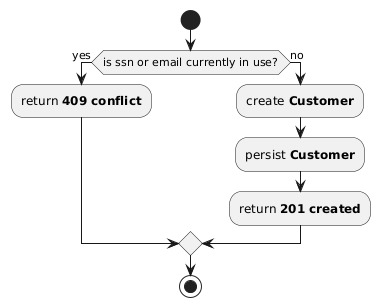
\includegraphics[width=1\linewidth]{figures/customer_registration_activity_diagram.png}
	\label{fig:customer_registration_flow}
	\footnotesize Source: Author's creation.
\end{figure}

If the verification discovers that the provided SSN or email is already associated with a persisted \textbf{Person} within a \textbf{Person}, the \hyperref[tab:summary_http_status_codes]{status code 409} is thrown. Otherwise, a new instance of \textbf{Customer} is created,  persisted, and the \hyperref[tab:summary_http_status_codes]{status code 201} is thrown. The more detailed flow shall be displayed in the sequence diagram present in the figure \ref{fig:customer_registration_sequence_diagram}.

A sequence diagram (or event diagram) models the behavioral aspects of a model. It projects the way objects interact with each other and exchange the messages among each other using parallel vertical lines called lifelines and horizontal arrows that show the messages exchanged between the objects, also telling about when to send what messages \cite{panigrahi2018}.

The figure \ref{fig:customer_registration_sequence_diagram} shows the sequence diagram of the registration of a Customer, as described in the \hyperref[subsection:http_semantics]{subsection HTTP Semantics}.

\begin{figure}[H]
	\centering
	\caption{Customer Registration Sequence Diagram}
	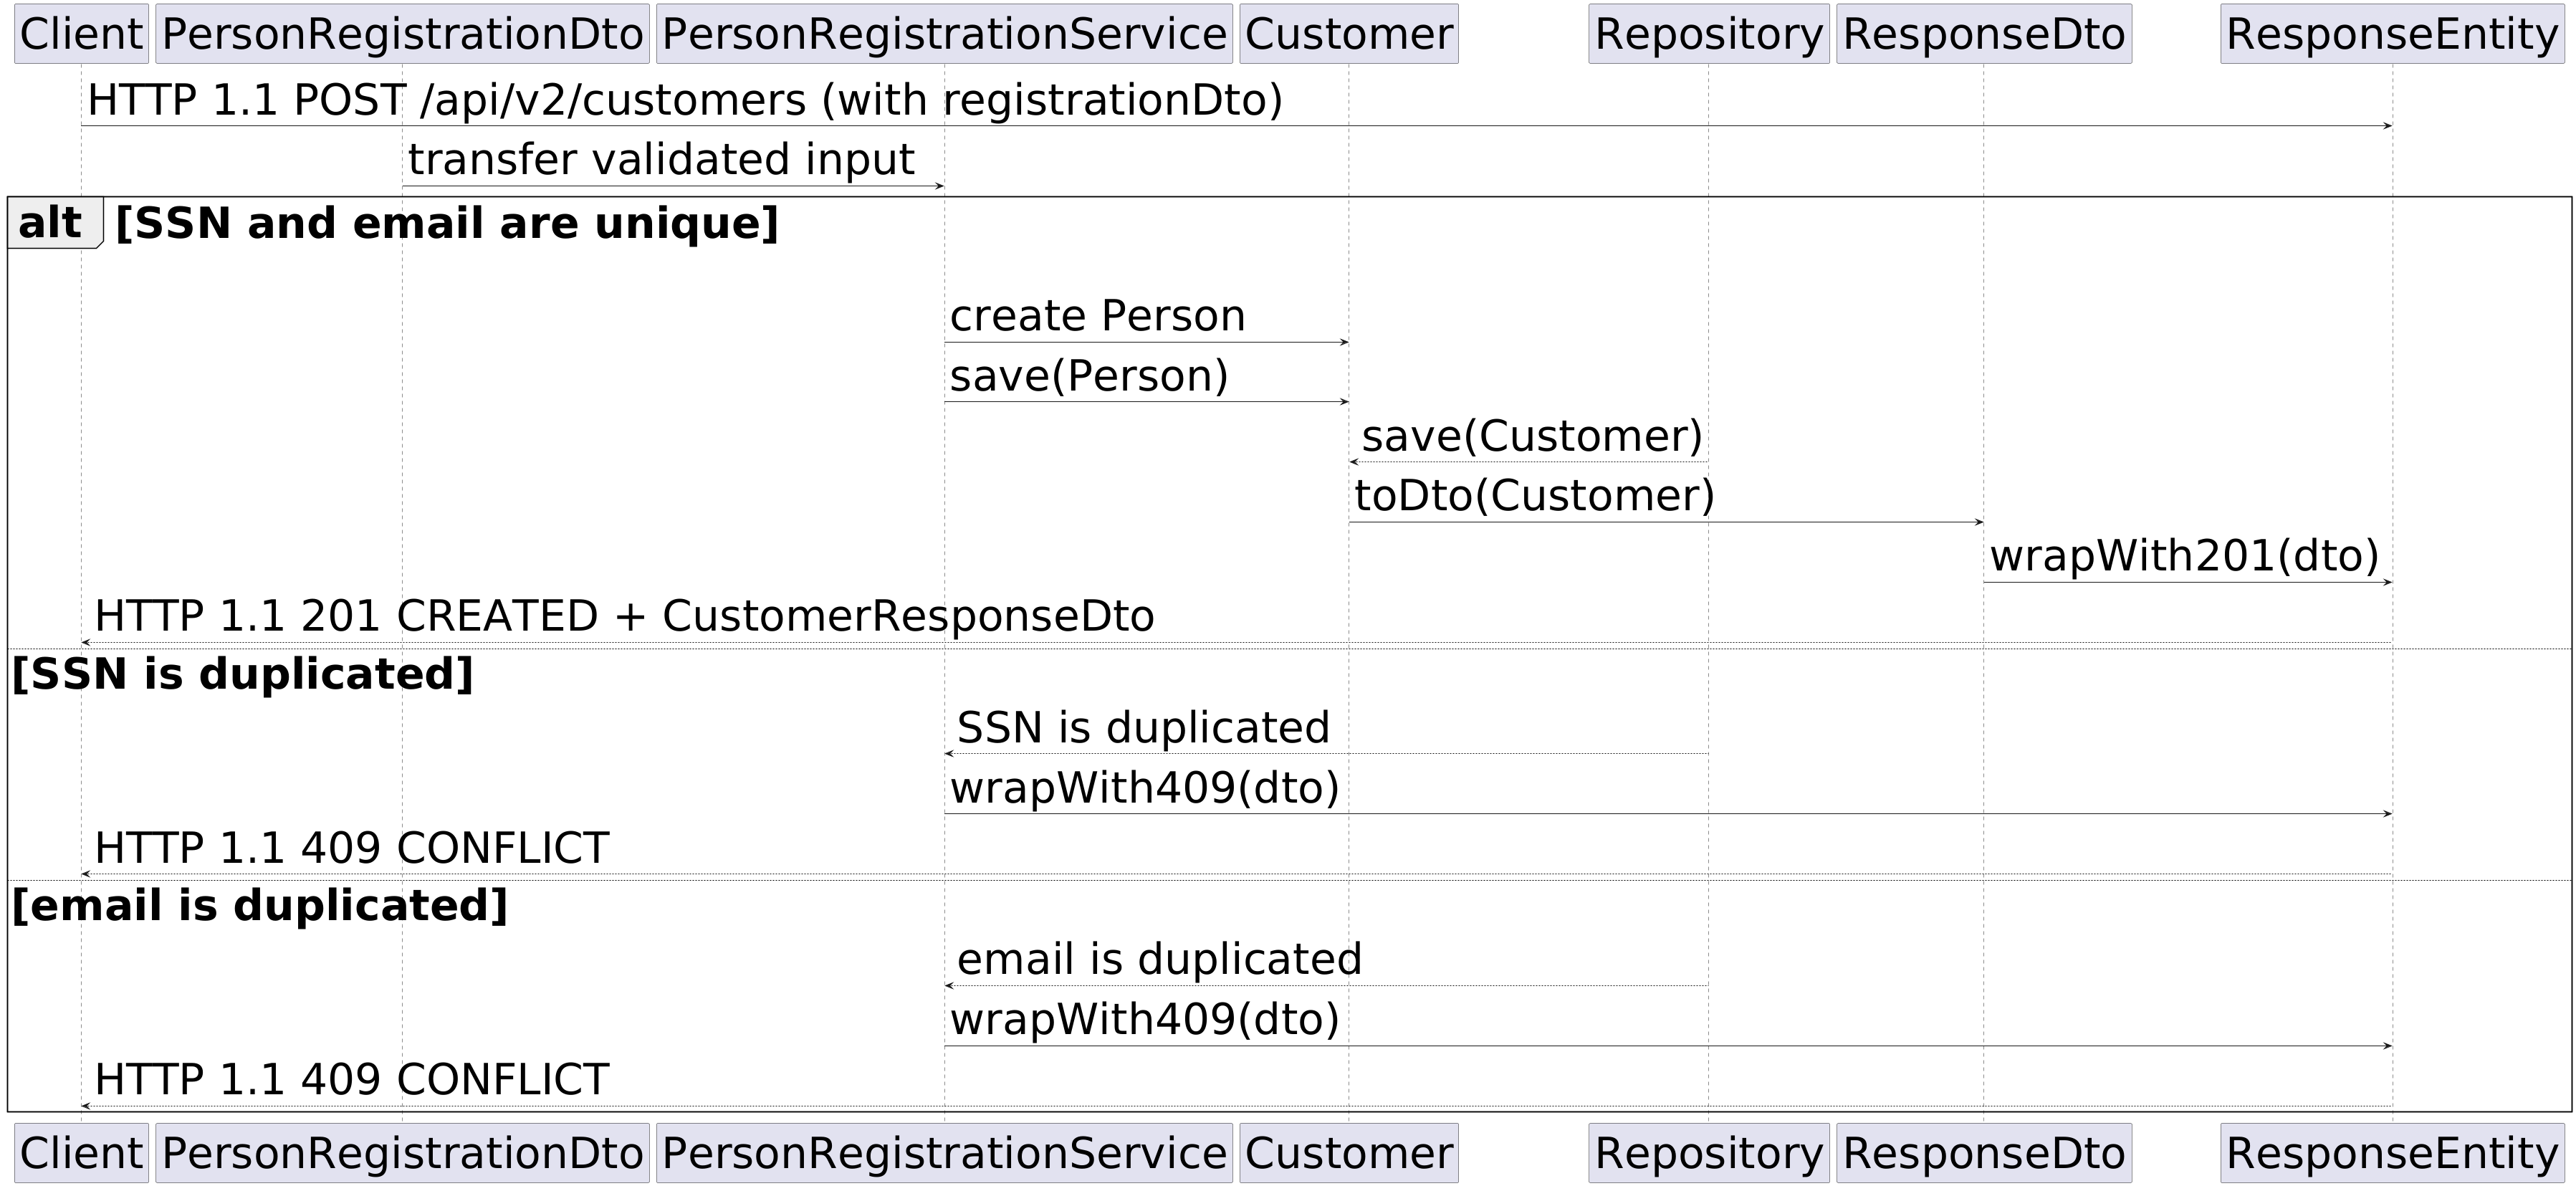
\includegraphics[width=1\linewidth]{figures/customer_registration_sequence_diagram.png}
	\\ \footnotesize Source: Author's creation.
	\label{fig:customer_registration_sequence_diagram}
\end{figure}

The client, whose behavior is described in the \hyperref[subsection:http_semantics]{subsection HTTP Semantics}, requests a resource. It uses the \hyperref[appendix:glossary]{URI} \textit{/api/v2/customers} with the body \textit{PersonRegistrationDto}. The \hyperref[appendix:glossary]{URI} follows the pattern established  in the table \ref{tab:http-server-schemes}.

The body is passed to the \textit{PersonRegistrationService} as its parameter. The service creates a new \textbf{Person}, then persists it.  The process of creating and persisting a \textbf{Person} follows what the \hyperref[core_person_registration_process]{section Core Person Registration Process} states.

As \textbf{Person} is embedded in \textbf{Customer}, as shown by the ERD diagram (figure \ref{fig:erd}). \textit{CustomerRepository} persists the recently created \textbf{Customer} and it is mapped into a \hyperref[appendix:glossary]{DTO} named \textit{CustomerResponseDto}. The \hyperref[appendix:glossary]{DTO} is wrapped in the \textit{ResponseEntity}, that returns the \hyperref[tab:summary_http_status_codes]{status code 201} alongside the \textit{CustomerResponseDto}.

As stated by the \hyperref[subsection:automated_software_testing]{subsection Automated Software Testing}, the test case contains a \hyperref[appendix:glossary]{DTO} \textit{CustomerRegistrationDto}, which has an embedded \hyperref[appendix:glossary]{DTO} \textit{PersonRegistrationDto}. The content of both \hyperref[appendix:glossary]{DTO} is demonstrated in the tables \ref{tab:customer_registration_dto} and \ref{tab:person_registration_dto}.

\begin{table}[H]
	\centering
	\caption{Fields in CustomerRegistrationDto}
	\begin{tabular}{ll}
		\toprule
		\textbf{Type} & \textbf{Variable Name} \\
		\midrule
		PersonRegistrationDto & personRegistrationDto \\ \hline
		Address & address \\
		\bottomrule
	\end{tabular}
	\\ \footnotesize Source: Author's creation.
	\label{tab:customer_registration_dto}
\end{table}

\begin{table}[H]
	\centering
	\caption{Fields in PersonRegistrationDto}
	\begin{tabular}{lll}
		\toprule
		\textbf{Type} & \textbf{Variable Name} & \textbf{Nullable} \\
		\midrule
		String & firstName & no \\ \hline
		String & middleName & yes \\ \hline
		String & lastName & no \\ \hline
		LocalDate & birthDate & no \\ \hline
		String & ssn & no \\ \hline
		String & email & no \\ \hline
		String & phoneNumber & no \\ \hline
		Gender & gender & no \\ \hline
		LocalDateTime & createdAt & no \\
		\bottomrule
	\end{tabular}
	\\ \footnotesize Source: Author's creation.
	\label{tab:person_registration_dto}
\end{table}

As the enum \textit{Gender} is mentioned in the table \ref{tab:person_registration_dto}, its content is described in the table \ref{tab:gender}.

\begin{table}[H]
	\centering
	\caption{Enum Gender}
	\begin{tabular}{l}
		\toprule
		\textbf{Gender} \\
		\midrule
		CIS\_MALE \\ \hline
		CIS\_FEMALE \\ \hline
		TRANS\_MALE \\ \hline
		TRANS\_FEMALE \\ \hline
		QUEER \\ \hline
		NON\_BINARY \\ \hline
		OTHER \\
		\bottomrule
	\end{tabular}
	\\ \footnotesize Source: Author's creation.
	\label{tab:gender}
\end{table}

Moreover, as the \hyperref[appendix:glossary]{DTO} \textit{Address} is the table \ref{tab:person_registration_dto}, its content is described in the table \ref{tab:address}. The given \hyperref[appendix:glossary]{DTO} contains an address that follows the US address model. The gender options presented are increasingly recognized and used in data collection within Western liberal democracies like the US, Canada, and the UK, reflecting a growing societal awareness of diverse gender identities, aiming for a more inclusive representation.

\begin{table}[H]
	\centering
	\caption{Fields in Address}
	\begin{tabular}{lll}
		\toprule
		\textbf{Type} & \textbf{Variable Name} & \textbf{Nullable} \\
		\midrule
		States & state & no \\ \hline
		String & city & no \\ \hline
		String & street & no \\ \hline
		String & zipcode & no \\
		\bottomrule
	\end{tabular}
	\\ \footnotesize Source: Author's creation.
	\label{tab:address}
\end{table}

As part of \textit{Address}, the enum \textit{States}'s content is descrided in the figure \ref{fig:states}. The given enum contains all the US states, excluding the US territories.

\begin{figure}[H]
	\centering
	\caption{Enum States}
	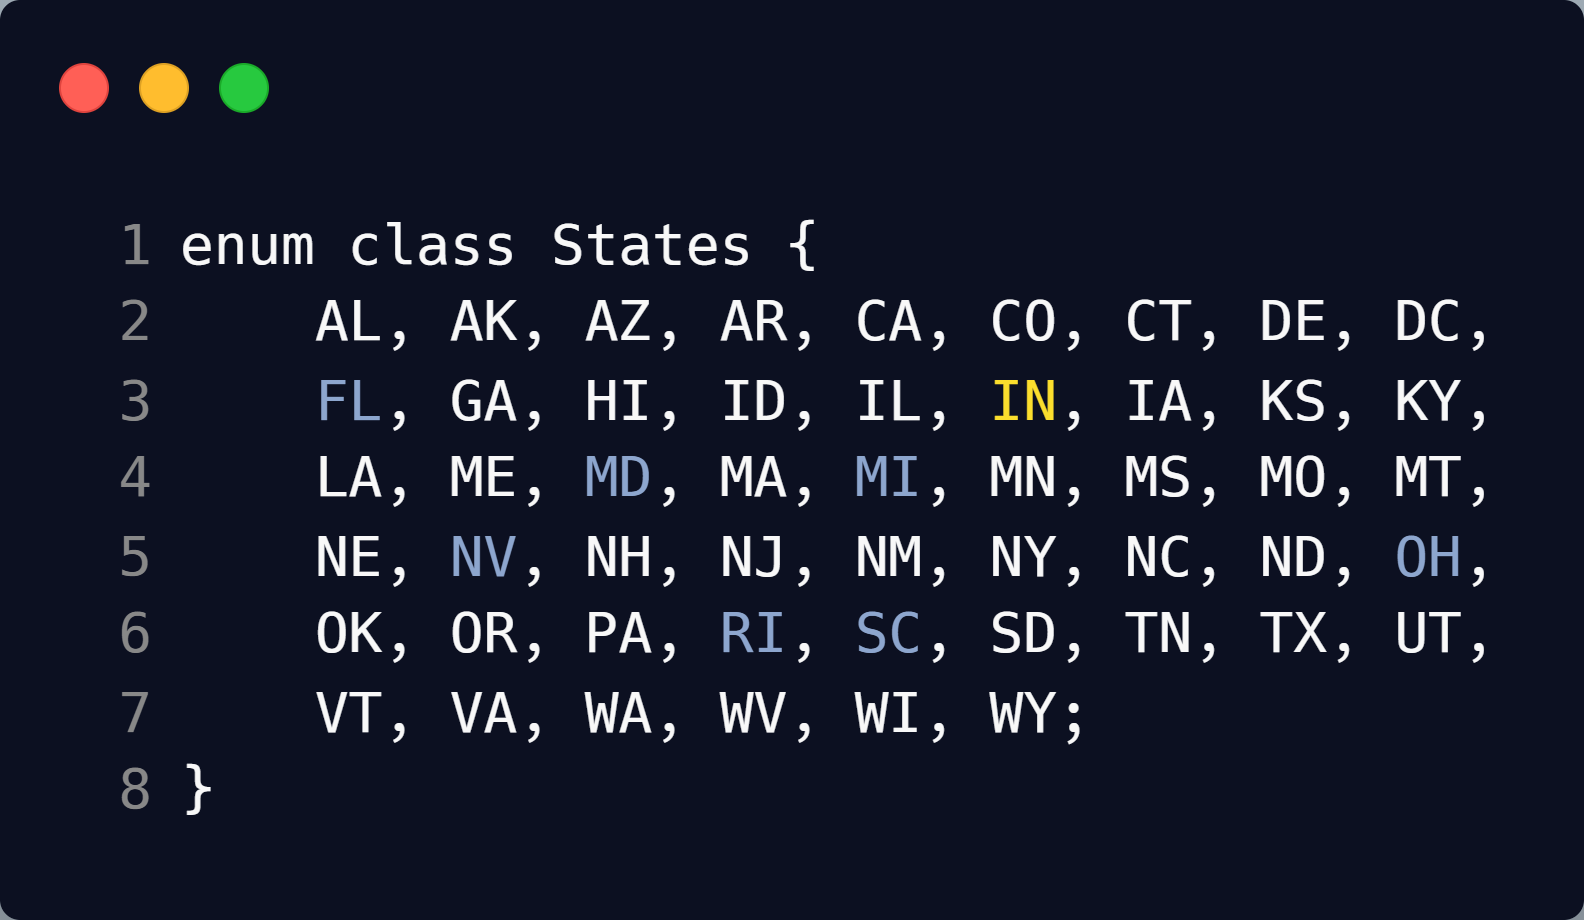
\includegraphics[width=1\linewidth]{figures/states_enum.png}
	\footnotesize Source: Author's creation.
	\label{fig:states}
\end{figure}

Finally, the testing class name \textit{CustomerRegistrationIntegrationTest} contains 
three methods:

\begin{enumerate}
	\item testSuccessfulRegistration.
	\item testUnsuccessfulRegistration\_Duplicated\_Ssn.
	\item testUnsuccessfulRegistration\_Duplicated\_Email
\end{enumerate}

\subsubsection{Successful Case}
\label{customer_registration_successful_test}

The method \textit{testSuccessfulRegistration} is success-oriented. The given method is represented in the figure \ref{fig:customer_registration_integration_test_success}. 

\begin{figure}[H]
	\centering
	\caption{Customer Registration Successful Integration Test}
	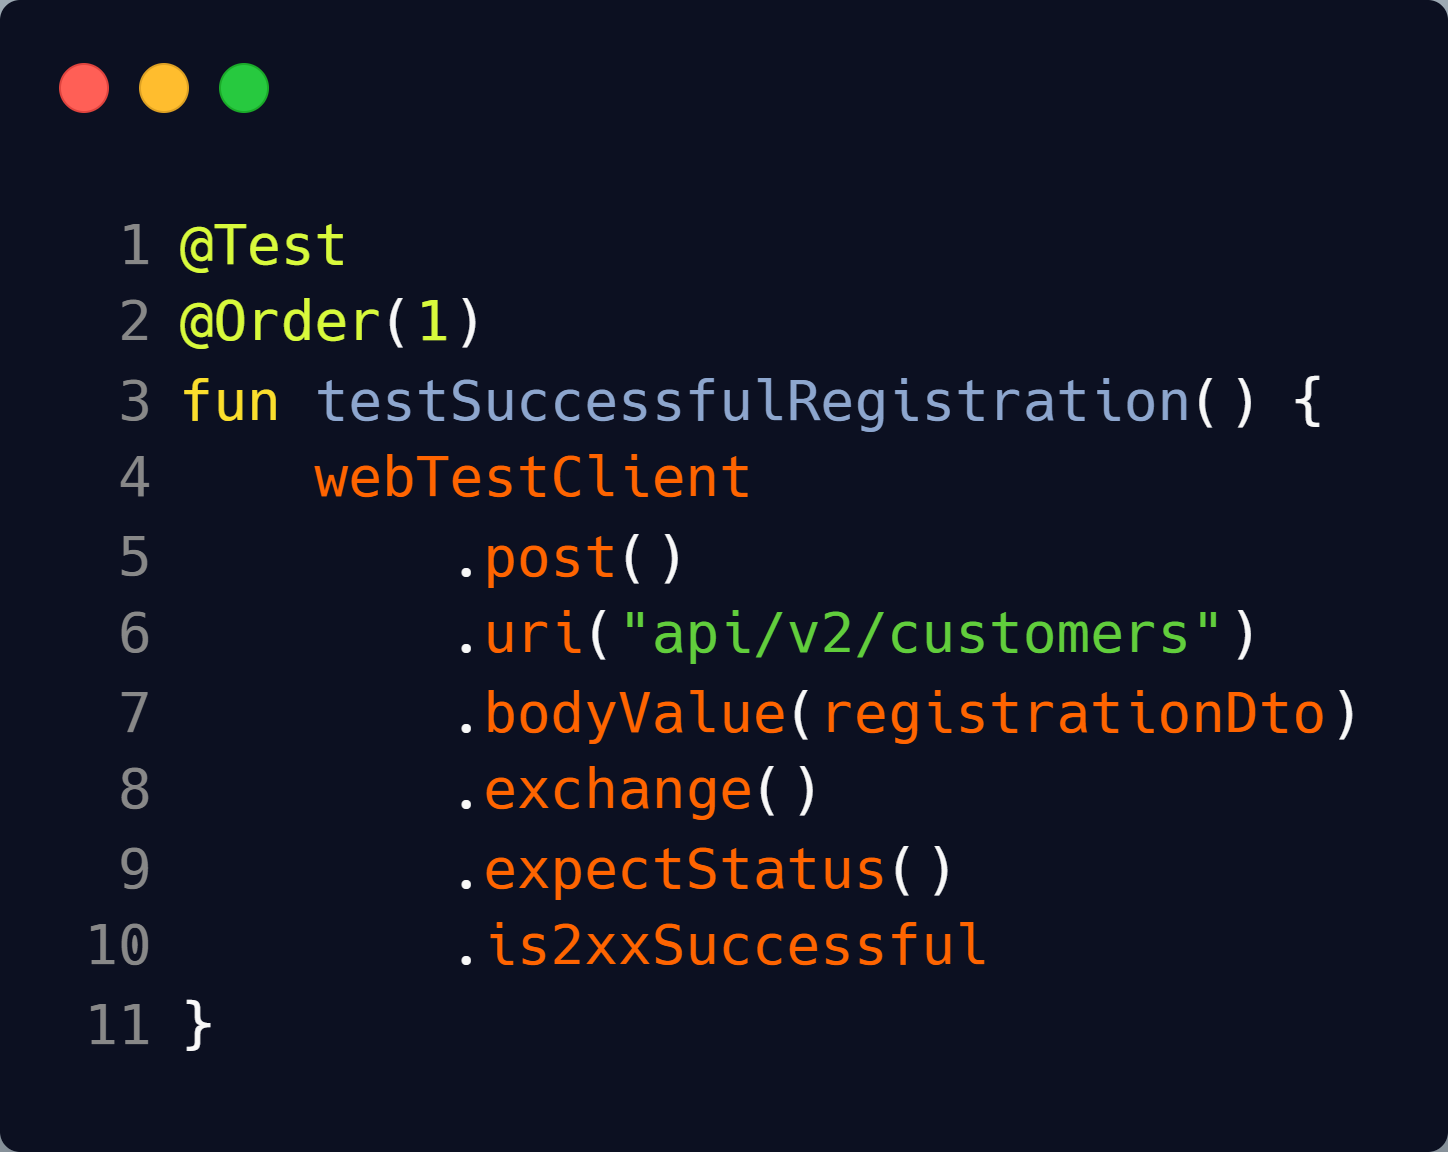
\includegraphics[width=1\linewidth]{figures/customer_registration_integration_test_success.png}
	\label{fig:customer_registration_integration_test_success}
	\\ \footnotesize Source: Author's creation.
\end{figure}

The method \textit{testSuccessfulRegistration} uses an instance of the \textit{WebTestClient}, as argued by the \hyperref[subsection:automated_software_testing]{subsection Automated Software Testing}. In order to register a \textbf{Customer}, the POST method was used. As clarified by the \hyperref[subsection:http_semantics]{subsection HTTP Semantics}, every HTTP request requires \hyperref[appendix:glossary]{URI} to route the expected request to the target server aiming to obtain the expected result. Thereby, the \hyperref[appendix:glossary]{URI} \textit{/api/v2/customers} is placed as the argument of \textit{uri()} and the \hyperref[appendix:glossary]{DTO} mentioned in the table \ref{tab:customer_registration_dto} as the request's body is placed as the parameter of \textit{bodyValue()}. Finally, the \hyperref[tab:summary_http_status_codes]{status code 201} is returned.

\subsubsection{Unsuccessful Case: Duplicated SSN}
\label{customer_registration_unsuccessful_test_duplicated_ssn}

\begin{figure}[H]
	\centering
	\caption{Customer Registration Integration Unsuccessful Test: Duplicated SSN}
	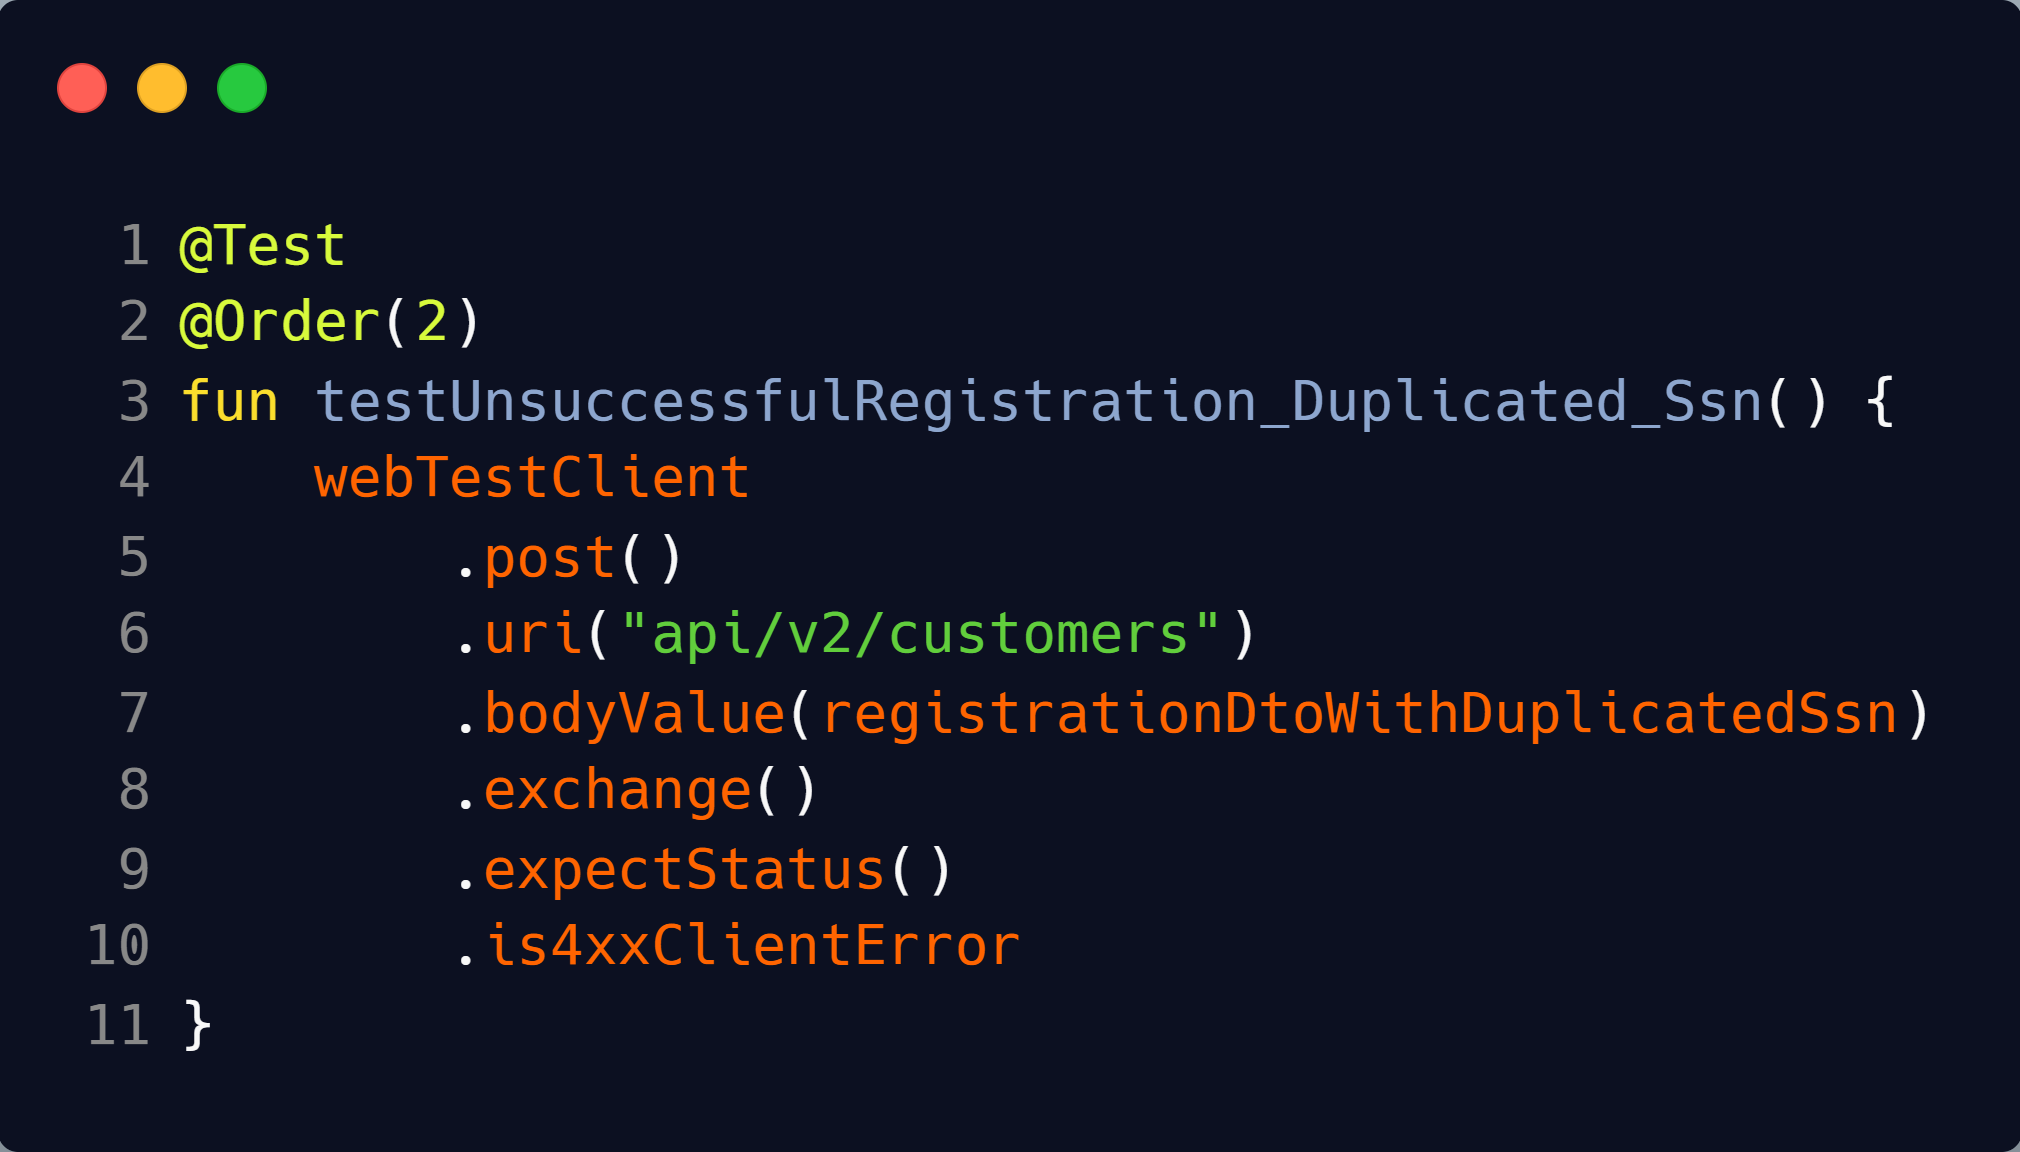
\includegraphics[width=1\linewidth]{figures/customer_registration_integration_test_unsuccess_duplicated_ssn.png}
	\label{fig:customer_registration_integration_test_unsuccess_duplicated_ssn}
	\footnotesize Source: Author' creation.
\end{figure}

The method \textit{testUnsuccessfulRegistration\_Duplicated\_Ssn} uses an instance of \textit{WebTestClient}, as argued by the \hyperref[subsection:automated_software_testing]{subsection Automated Software Testing}. When, at the moment that validated input data is extracted from the \hyperref[appendix:glossary]{DTO} (table \ref{tab:customer_registration_dto}), if it is discovered that the provided SSN is in use in another \textbf{Person} associated with a \textbf{Customer} (see figure \ref{fig:customer_registration_sequence_diagram}), the \hyperref[tab:summary_http_status_codes]{status code 409} is returned.

\subsubsection{Unsuccessful Case: Duplicated Email}
\label{customer_registration_unsuccessful_test_duplicated_email}

\begin{figure}[H]
	\centering
	\caption{Customer Registration Integration Test Unsuccess: Duplicated Email}
	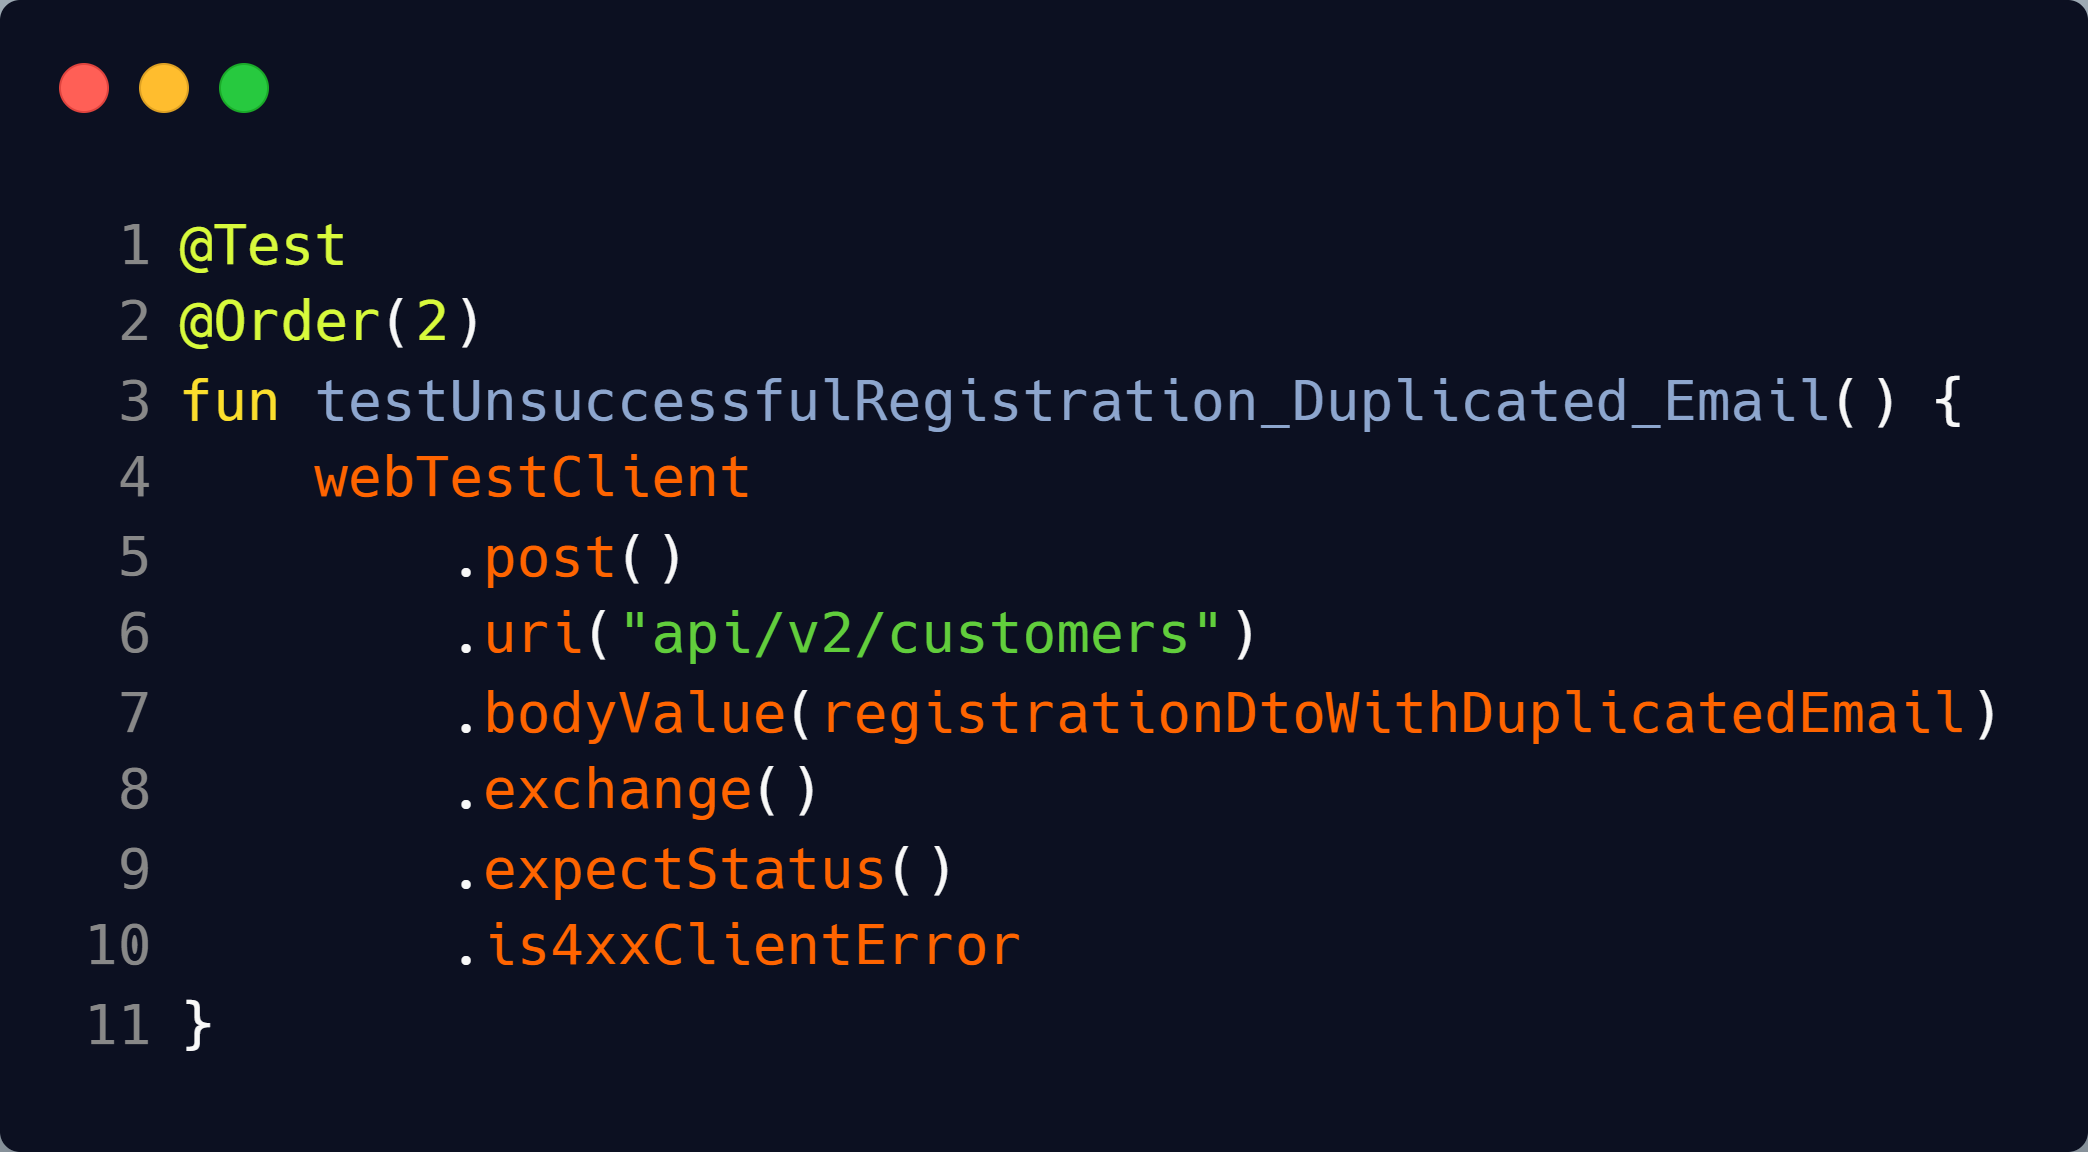
\includegraphics[width=1\linewidth]{figures/customer_registration_integration_test_unsuccess_duplicated_email.png}
	\label{fig:customer_registration_integration_test_unsuccess_duplicated_email} 
	\\ \footnotesize Source: Author' creation.
\end{figure}

The method \textit{testUnsuccessfulRegistration\_Duplicated\_Email} uses an instance of the \textit{WebTestClient}, as argued by the \hyperref[subsection:automated_software_testing]{subsection Automated Software Testing}. When, at the moment that validated input data is extracted from the \hyperref[appendix:glossary]{DTO} (table \ref{tab:customer_registration_dto}) and it is discovered that the provided email is in use in another \textbf{Person} associated with a \textbf{Customer} (see figure \ref{fig:customer_registration_sequence_diagram}), the \hyperref[tab:summary_http_status_codes]{status code 409} is returned.

\subsubsection{Summary of Results}

\begin{figure}[H]
	\centering
	\caption{Customer Registration Integration Test's Results}
	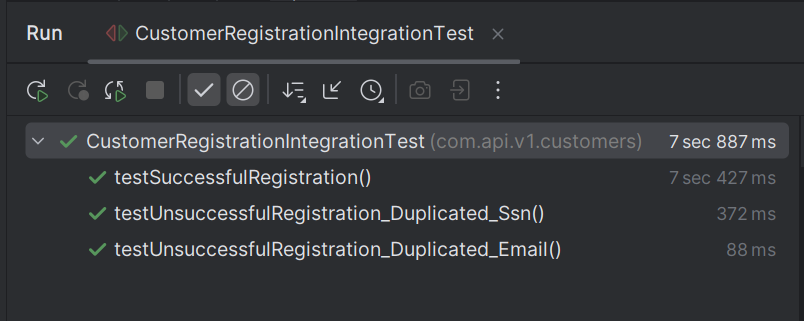
\includegraphics[width=1\linewidth]{figures/results_customer_registration_integration_test.PNG}
	\\ \footnotesize Source: Author's creation.
	\label{fig:results_customer_registration_integration_test}
\end{figure}

Methods of integration tests are expected to pass, reg rdless of the successful or unsuccessful representation of the endpoint's response, due to the fact that integration tests are supposed to represent the system's functionality.

\subsection{Doctor Registration}

The figure \ref{fig:doctor_registration_activity_diagram} is an activity diagram that shows visually the flow of the registration of a \textbf{Doctor}.
\begin{figure}[H]
	\centering
	\caption{Flow of the Registration of a Medical Slot}
	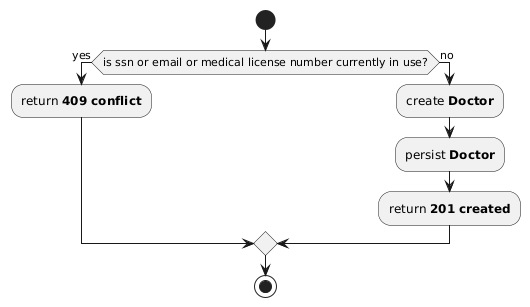
\includegraphics[width=1\linewidth]{figures/doctor_registration_activity_diagram.png}
	\\ \footnotesize Source: Author's creation.
	\label{fig:doctor_registration_activity_diagram}
\end{figure}

If the verification discovers that the provided SSN or email is already associated with a persisted \textbf{Person} within a \textbf{Doctor} or the provided medical license number is already associated with a \textbf{Doctor}, the \hyperref[tab:summary_http_status_codes]{status code 409} is thrown. Otherwise, a new instance of \textbf{Doctor} is created,  persisted, and the \hyperref[tab:summary_http_status_codes]{status code 201} is thrown. The more detailed flow shall be displayed in the sequence diagram present in the figure \ref{fig:doctor_registration_sequence_diagram}.

\begin{figure}[H]
	\centering
	\caption{Doctor Registration Sequence Diagram}
	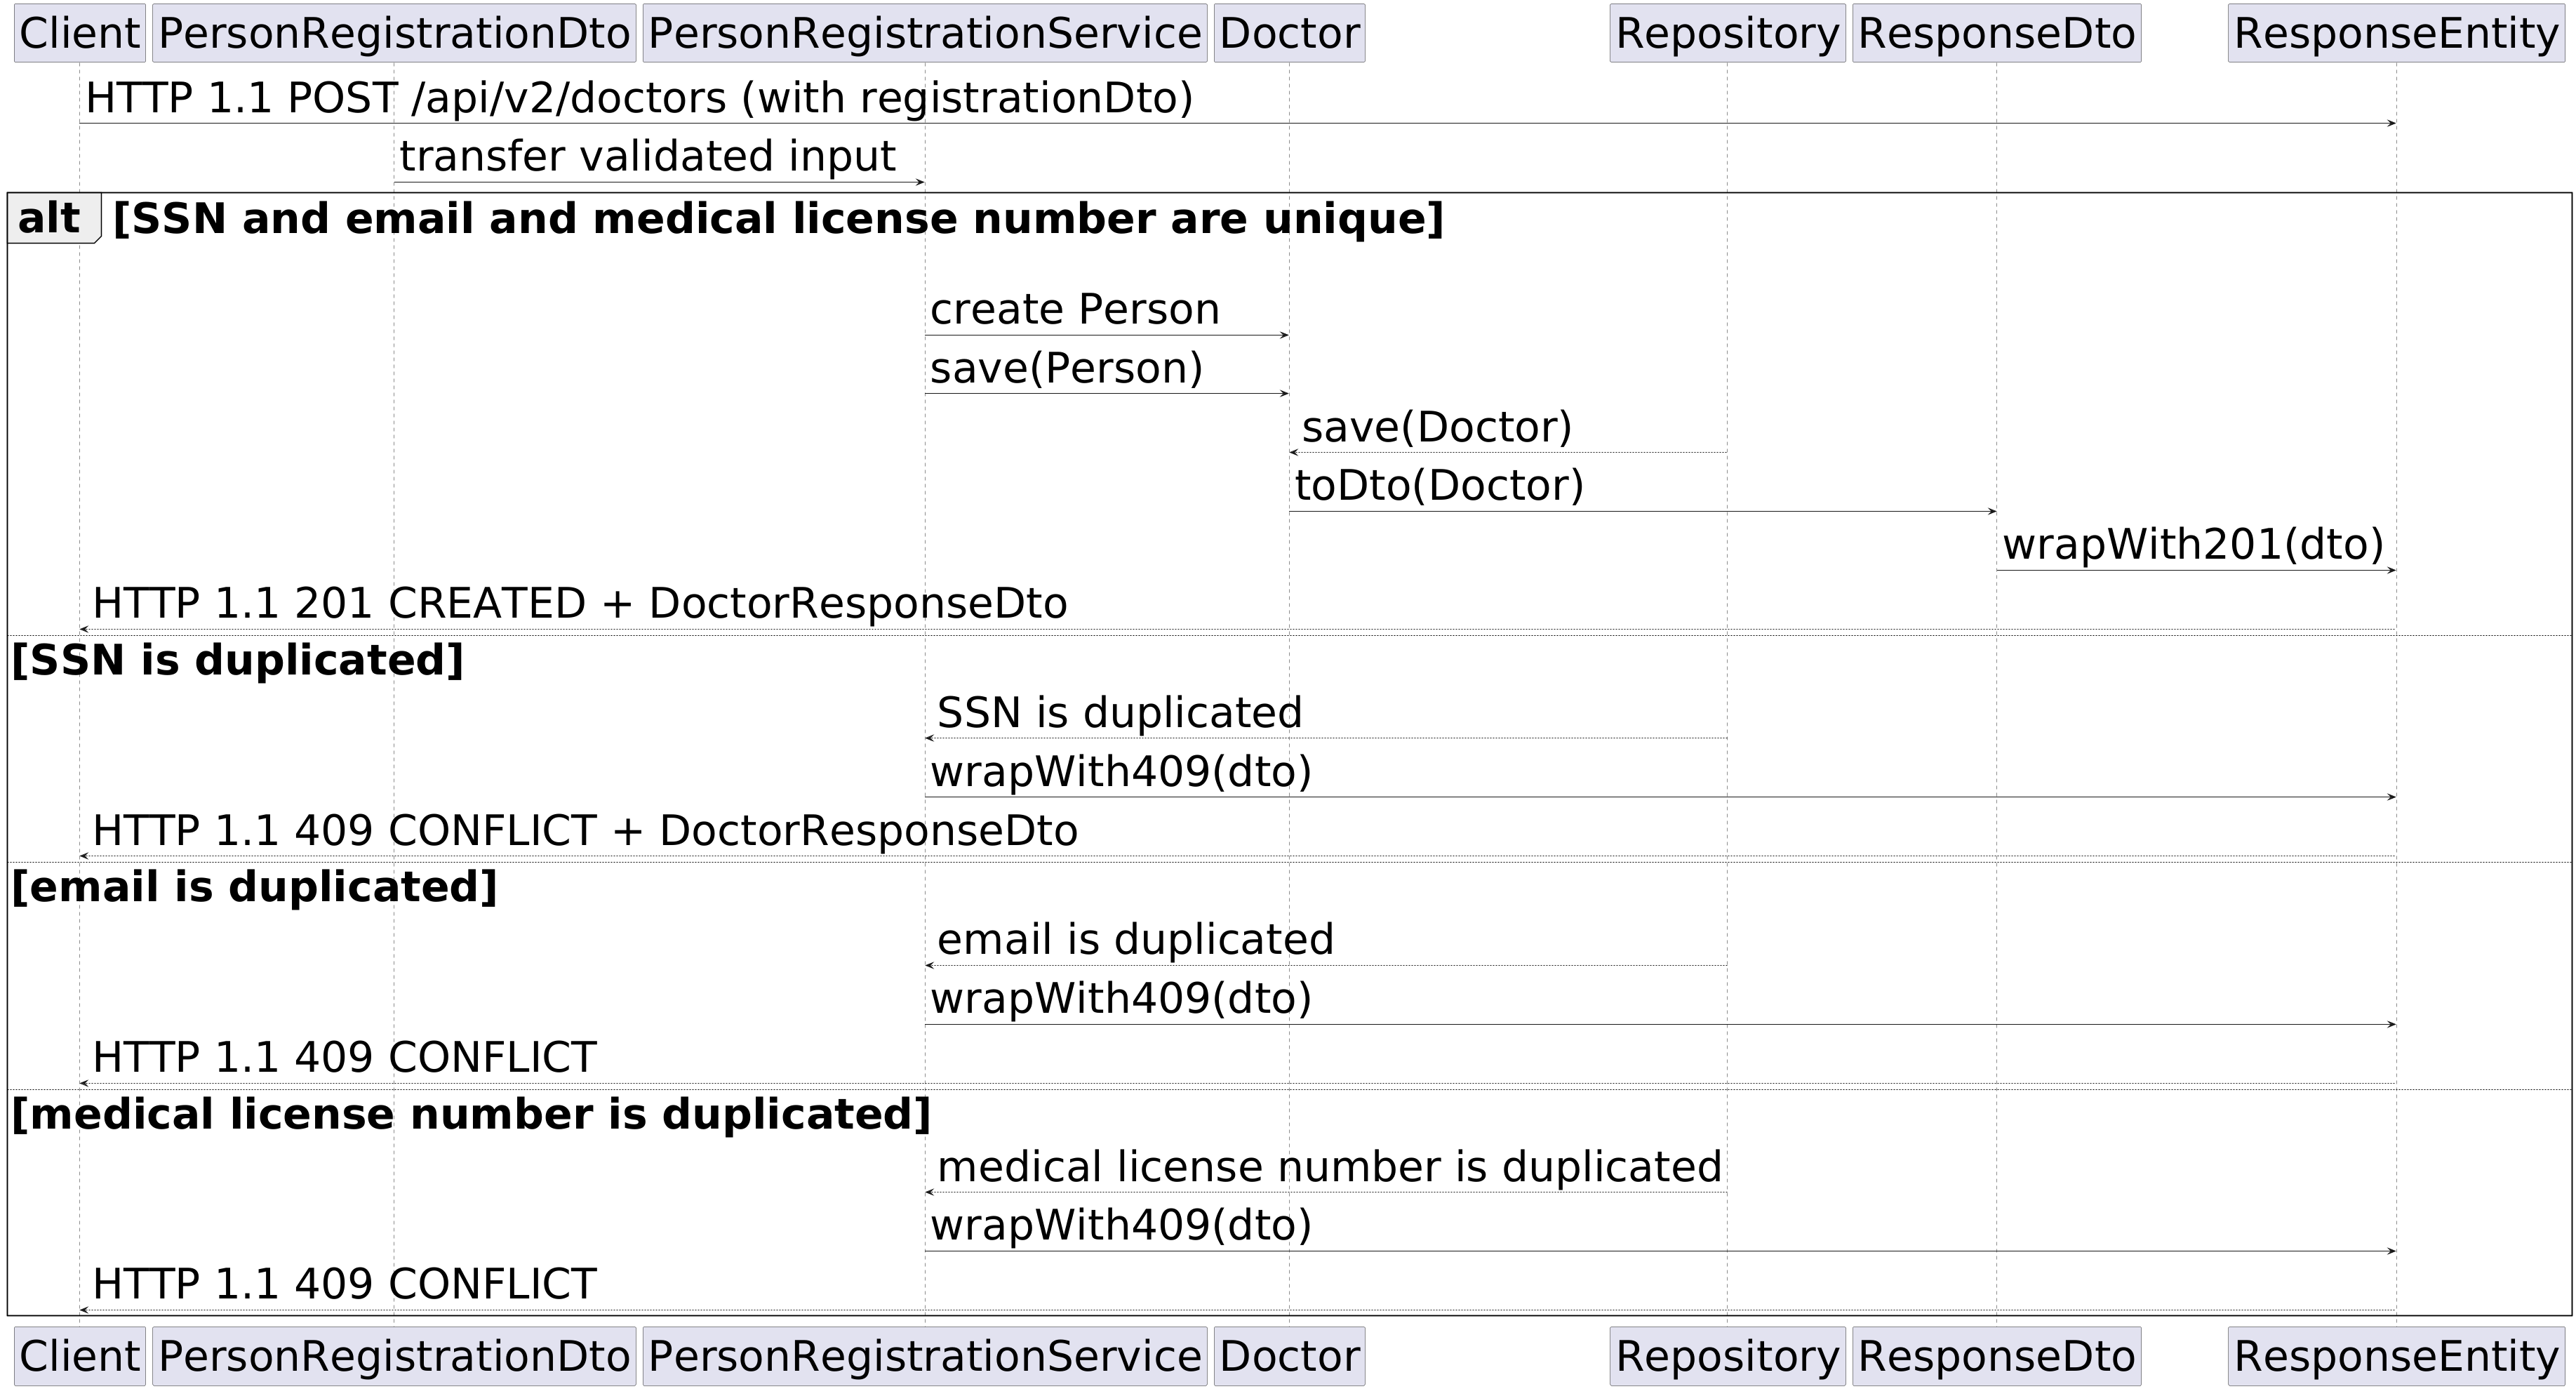
\includegraphics[width=1\linewidth]{figures/doctor_registration_sequence_diagram.png}
	\\ \footnotesize Source: Author's creation.
	\label{fig:doctor_registration_sequence_diagram}
\end{figure}

The client, whose behavior is described in the \hyperref[subsection:http_semantics]{subsection HTTP Semantics}, requests a resource. It uses the \hyperref[appendix:glossary]{URI} \textit{/api/v2/customers} with the body \textit{PersonRegistrationDto}. The \hyperref[appendix:glossary]{URI} follows the pattern established  in the table \ref{tab:http-server-schemes}.

The body is passed to the \textit{PersonRegistrationService} as its parameter. The service creates a new \textbf{Person}, then persists it. The process of creating and persisting a \textbf{Person} follows what the \hyperref[core_person_registration_process]{section Core Person Registration Process} states.
As \textbf{Person} is embedded in \textbf{Doctor}, as shown by the ERD diagram (figure \ref{fig:erd}). \textit{DoctorRepository} persists the recently created \textbf{Doctor} and it is mapped into a \hyperref[appendix:glossary]{DTO} named \textit{DoctorResponseDto}. The \hyperref[appendix:glossary]{DTO} is wrapped in the \textit{ResponseEntity}, that returns the \hyperref[tab:summary_http_status_codes]{status code 201} alongside the \textit{CustomerResponseDto}.

As stated by the \hyperref[subsection:automated_software_testing]{subsection Automated Software Testing}, the test case contains a \hyperref[appendix:glossary]{DTO} \textit{CustomerRegistrationDto}, which has an embedded \hyperref[appendix:glossary]{DTO} \textit{PersonRegistrationDto}. The content of both \hyperref[appendix:glossary]{DTO} is demonstrated in the tables \ref{tab:person_registration_dto} and \ref{tab:doctor_registration_dto}.

\begin{table}[H]
	\centering
	\caption{Fields in DoctorRegistrationDto}
	\begin{tabular}{ll}
		\toprule
		\textbf{Type} & \textbf{Variable Name} \\
		\midrule
		PersonRegistrationDto & personRegistrationDto \\ \hline
		MedicalLicenseNumber & medicalLicenseNumber \\
		\bottomrule
	\end{tabular}
	\\ \footnotesize Source: Author's creation.
	\label{tab:doctor_registration_dto}
\end{table}

The content of the \hyperref[appendix:glossary]{DTO} \textit{MedicalLicenseNumber} is represented in the table \ref{tab:medical_license_number}.

\begin{table}[H]
	\centering
	\caption{Fields in MedicalLicenseNumber}
	\begin{tabular}{ll}
		\toprule
		\textbf{Type} & \textbf{Variable Name} \\
		\midrule
		String & licenseNumber \\ \hline
		States & state \\
		\bottomrule
	\end{tabular}
	\\ \footnotesize Source: Author's creation.
	\label{tab:medical_license_number}
\end{table}

\subsubsection{Successful Case}

\begin{figure}[H]
	\centering
	\caption{Doctor Registration Successful Integration Test}
	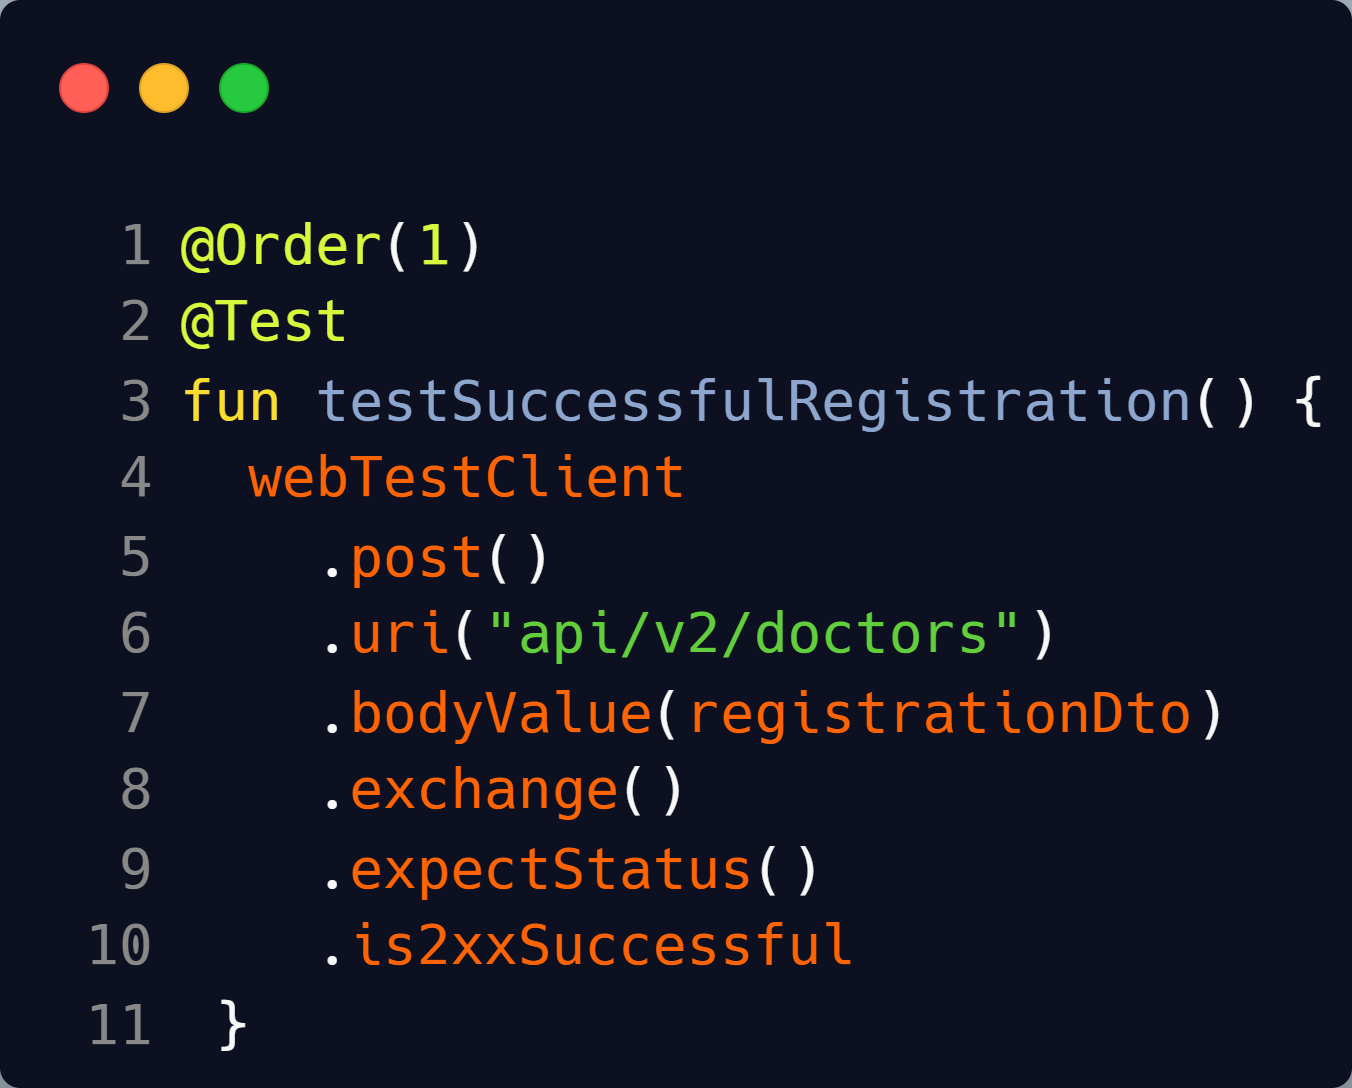
\includegraphics[width=1\linewidth]{figures/doctor_registration_integration_test_successful.png}
	\\ \footnotesize Source: Author's creation.
	\label{fig:doctor_registration_integration_test_successful}
\end{figure}

The method \textit{testSuccessfulRegistration} uses an instance of the \textit{WebTestClient}, as argued by the \hyperref[subsection:automated_software_testing]{subsection Automated Software Testing}. In order to register a \textbf{Doctor}, the POST method was used. As clarified by the \hyperref[subsection:http_semantics]{subsection HTTP Semantics}, every HTTP request requires \hyperref[appendix:glossary]{URI} to route the expected request to the target server aiming to obtain the expected result. Thereby, the \hyperref[appendix:glossary]{URI} \textit{/api/v2/doctors} is placed as the argument of \textit{uri()} and the \hyperref[appendix:glossary]{DTO} mentioned in the table \ref{tab:doctor_registration_dto} as the request's body is placed as the parameter of \textit{bodyValue()}. Finally, the \hyperref[tab:summary_http_status_codes]{status code 201} is returned.

\subsubsection{Unsuccessful Case: Duplicated Medical License Number}

\begin{figure}[H]
	\centering
	\caption{Doctor Registration Unsuccessful Case: Duplicated Medical License Number}
	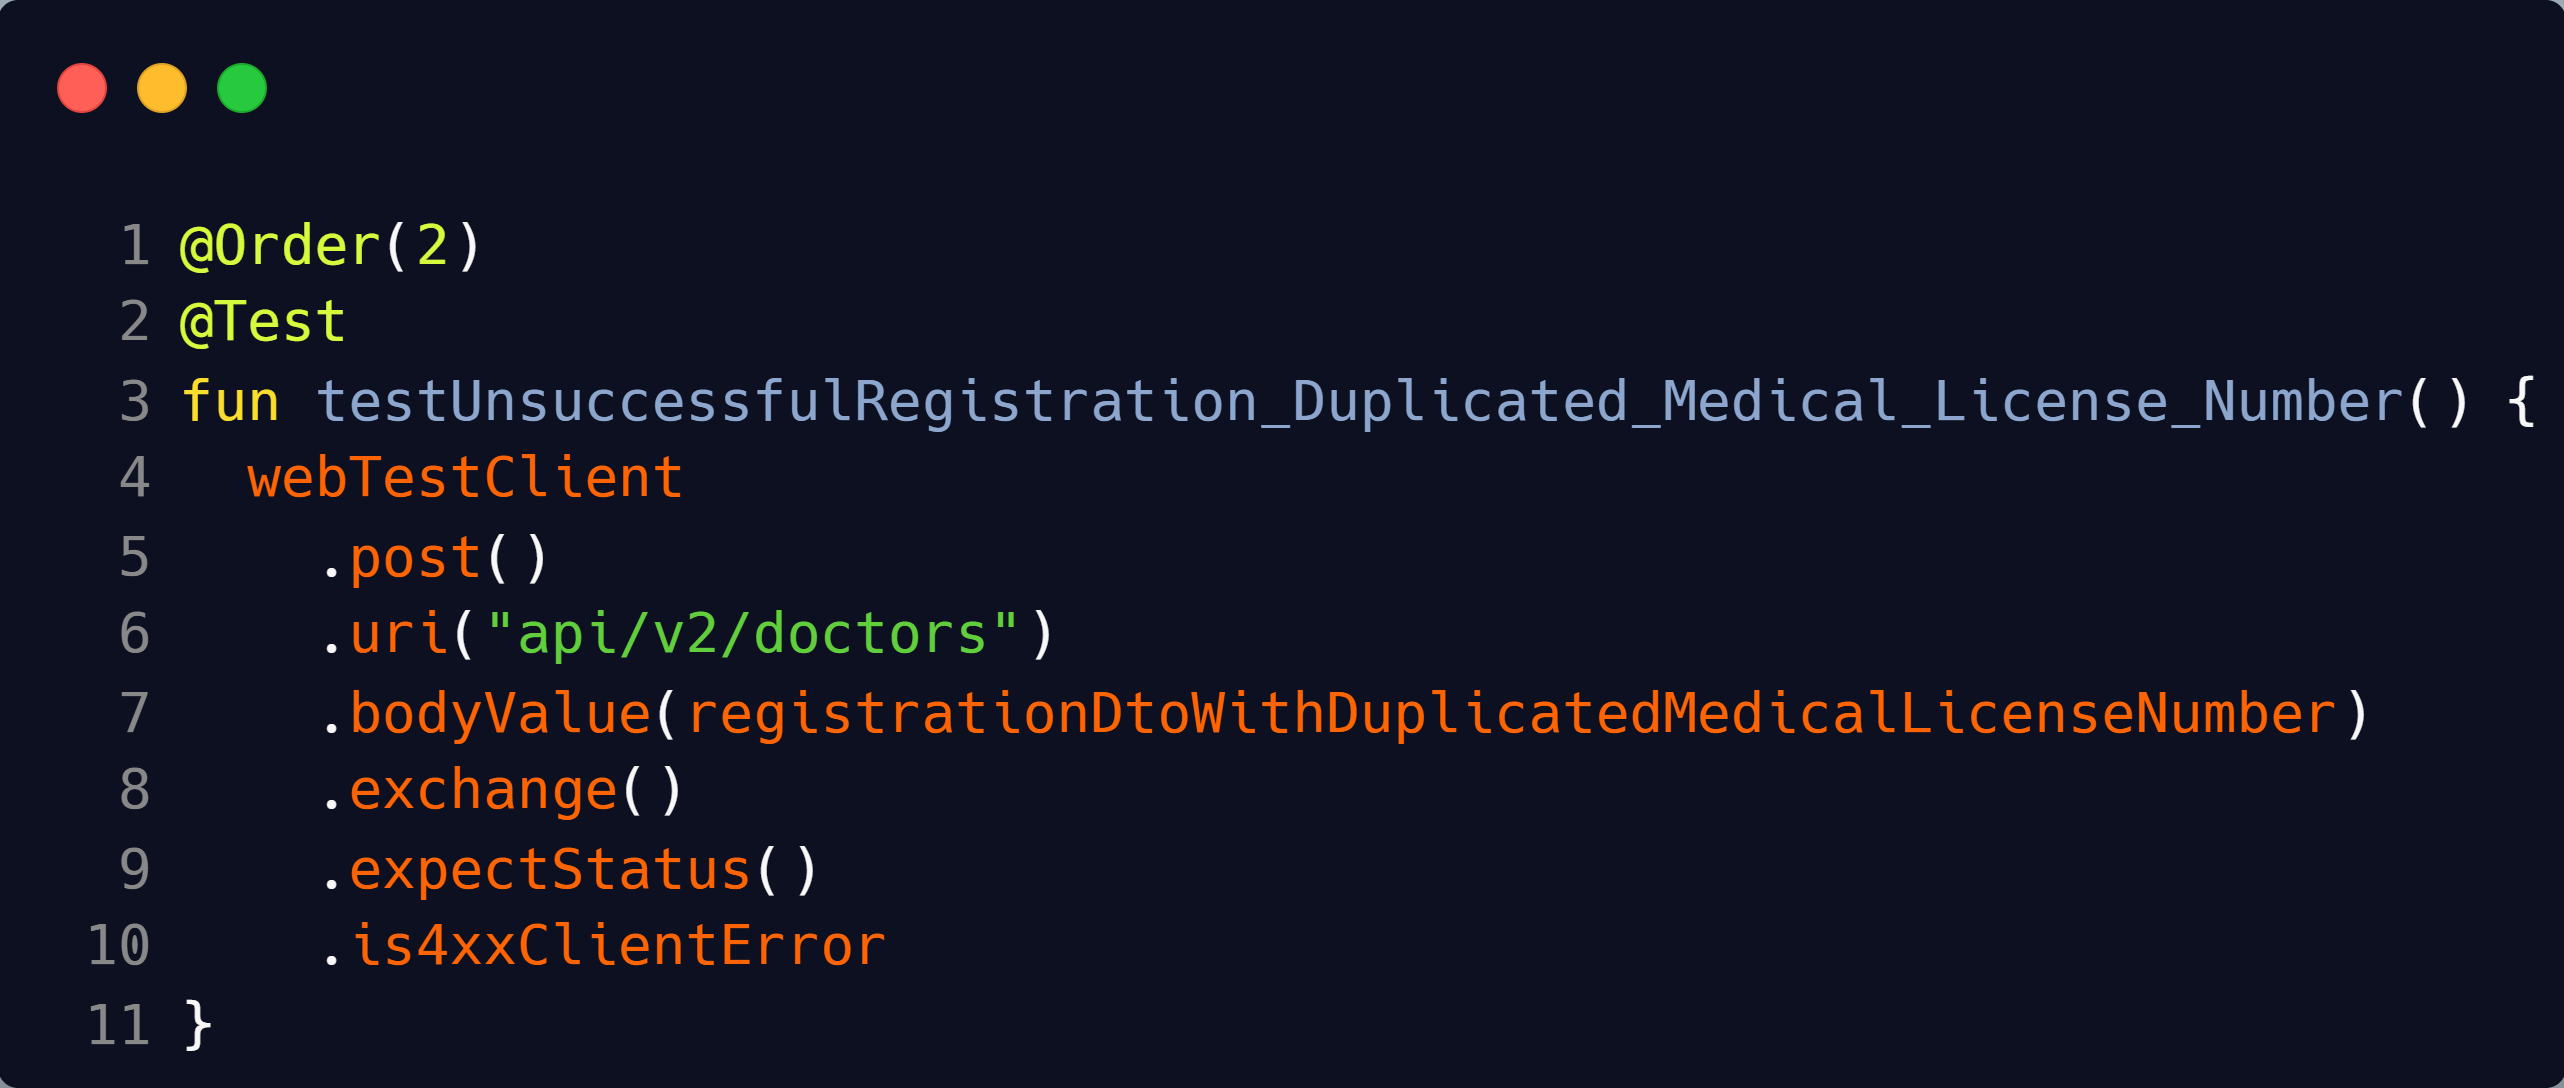
\includegraphics[width=1\linewidth]{figures/doctor_registration_unsucessful_integration_test_duplicated_mln.png}
	\\ \footnotesize Source: Author's creation.
	\label{fig:doctor_registration_unsucessful_integration_test_duplicated_mln}
\end{figure}

The method \textit{testUnsuccessfulRegistration\_Duplicated\_Medical\_License\_Number} uses an instance of the \textit{WebTestClient}, as argued by the \hyperref[subsection:automated_software_testing]{subsection Automated Software Testing}. When, at the moment that validated input data is extracted from the \hyperref[appendix:glossary]{DTO} (table \ref{tab:doctor_registration_dto}) and it is discovered that the provided medical license number is in use in an existing \textbf{Doctor} (see figure \ref{fig:doctor_registration_sequence_diagram}), the \hyperref[tab:summary_http_status_codes]{status code 409} is returned.

\subsubsection{Unsuccessful Case: Duplicated SSN}

\begin{figure}[H]
	\centering
	\caption{Doctor Registration Unsuccessful Case: Duplicated SSN}
	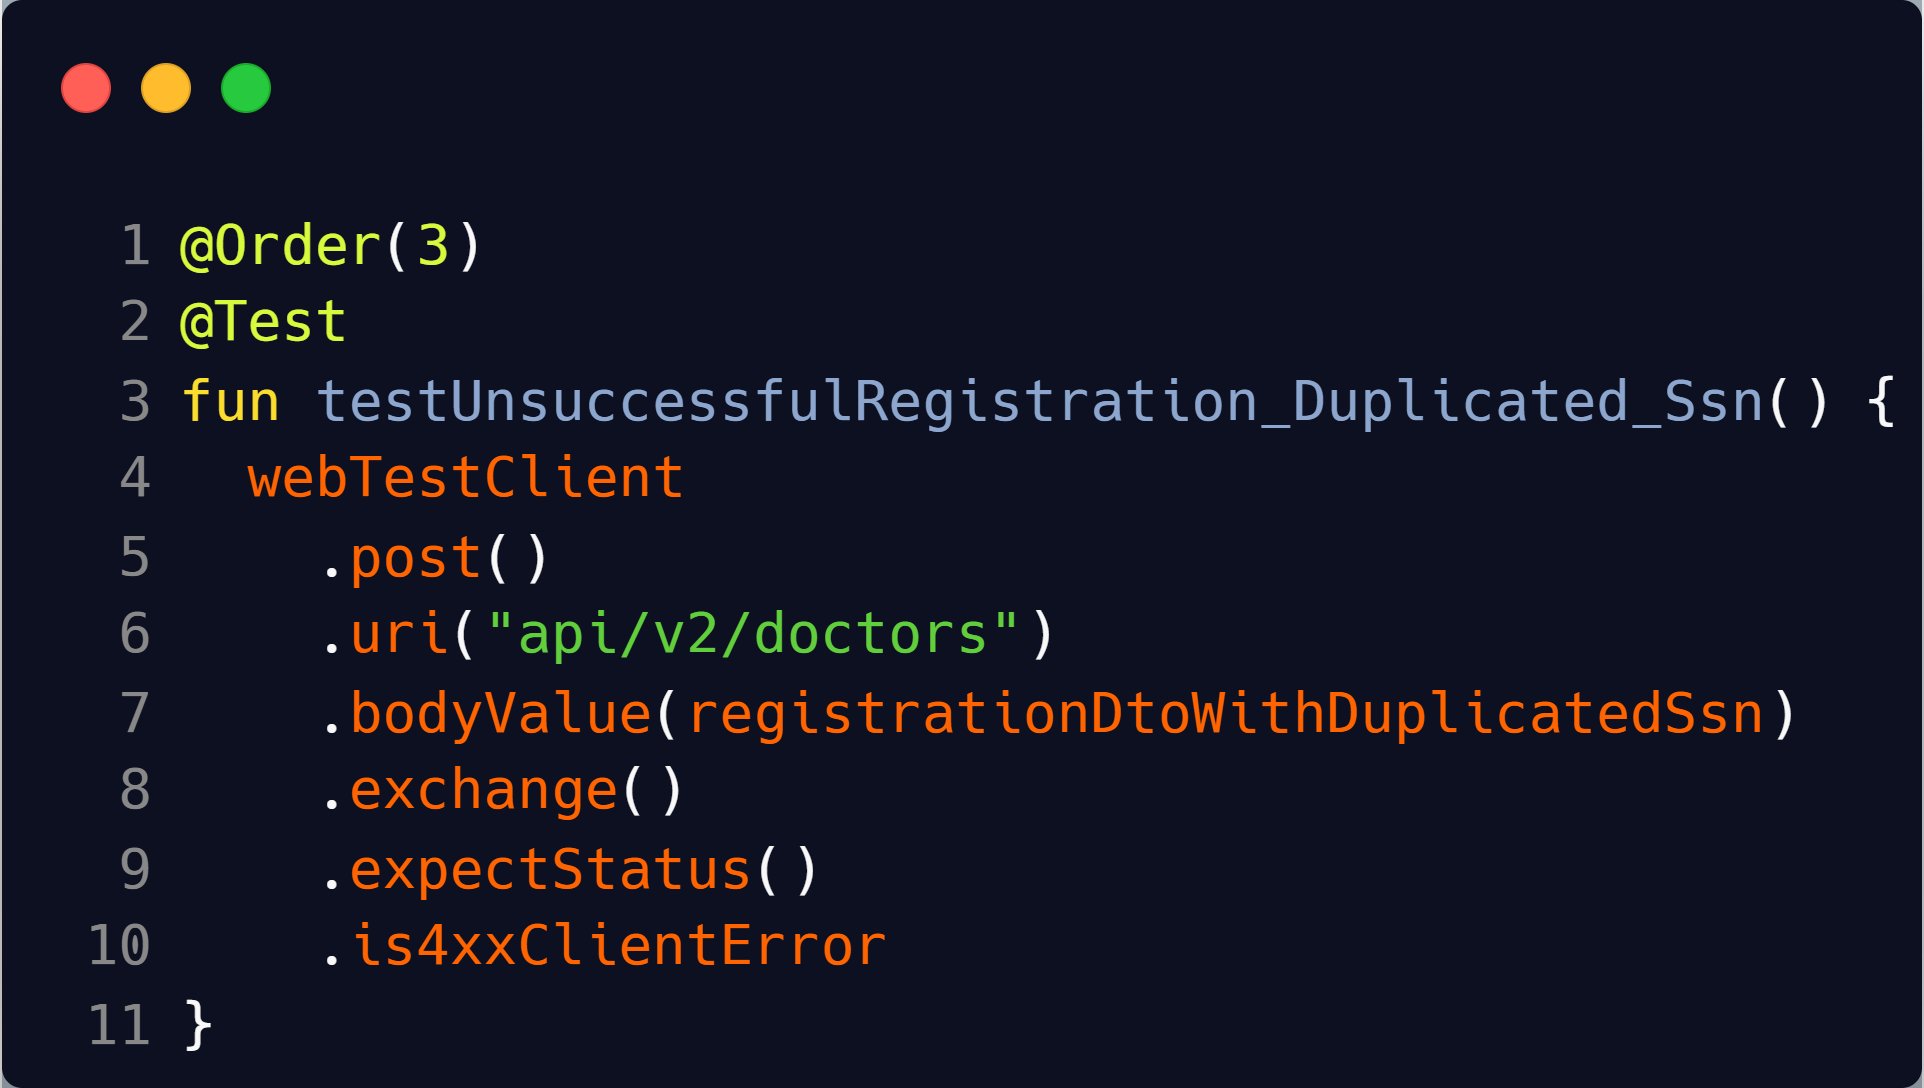
\includegraphics[width=1\linewidth]{figures/doctor_registration_unsucessful_integration_test_duplicated_ssn.png}
	\\ \footnotesize Source: Author's creation.
	\label{fig:doctor_registration_unsucessful_integration_test_duplicated_ssn}
\end{figure}

The method \textit{testUnsuccessfulRegistration\_Duplicated\_Ssn} uses an instance of the framework \textit{WebTestClient}, as argued by the \hyperref[subsection:automated_software_testing]{subsection Automated Software Testing}. When, at the moment that validated input data is extracted from the \hyperref[appendix:glossary]{DTO} (table \ref{tab:doctor_registration_dto}) and it is discovered that the provided SSN is in use in an embedded \textbf{Person} within a \textbf{Doctor} (see figure \ref{fig:doctor_registration_sequence_diagram}), the \hyperref[tab:summary_http_status_codes]{status code 409} is returned.


\subsubsection{Unsuccessful Case: Duplicated Email}

\begin{figure}[H]
	\centering
	\caption{Doctor Registration Unsuccessful Case: Duplicated Email}
	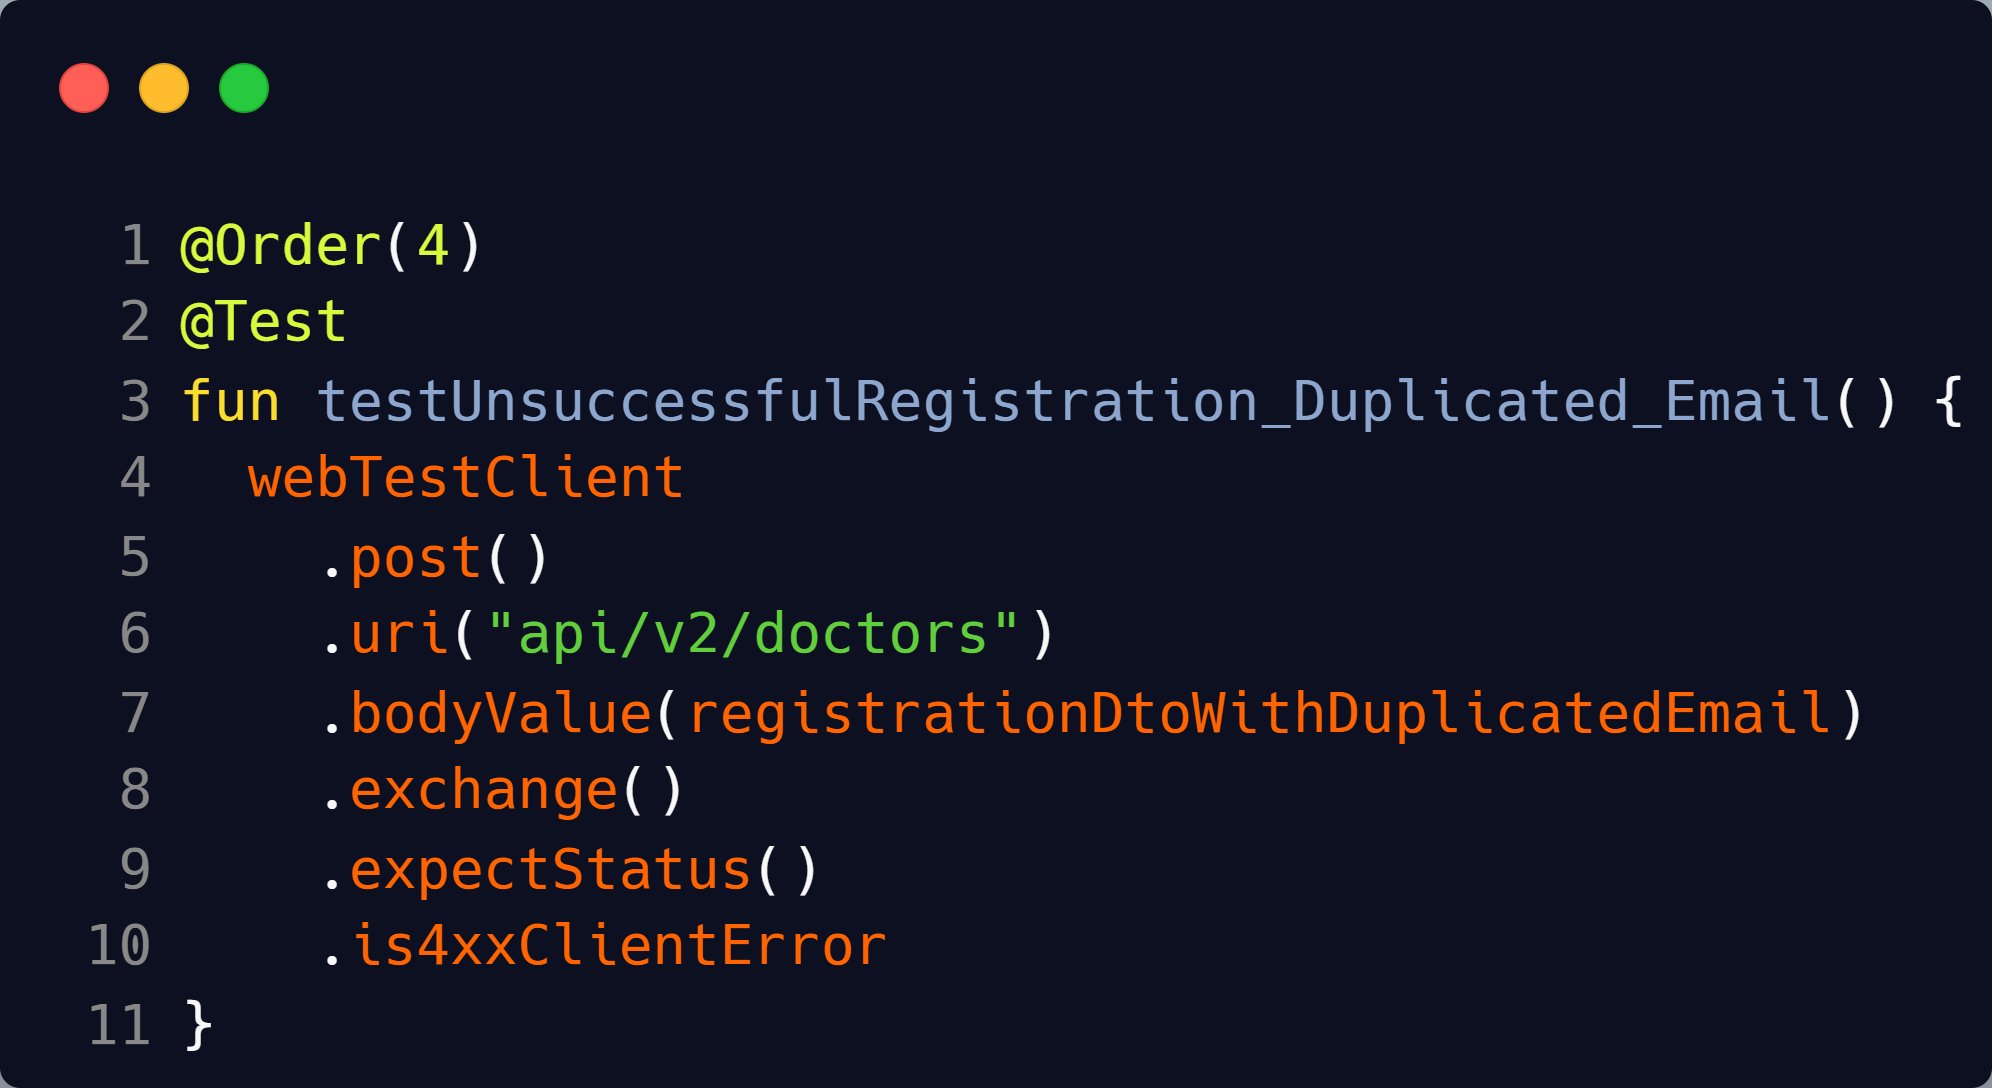
\includegraphics[width=1\linewidth]{figures/doctor_registration_unsucessful_integration_test_duplicated_email.png}
	\\ \footnotesize Source: Author's creation.
	\label{fig:doctor_registration_unsucessful_integration_test_duplicated_email}
\end{figure}

The method \textit{testUnsuccessfulRegistration\_Duplicated\_Email} uses an instance of the \textit{WebTestClient}, as argued by the \hyperref[subsection:automated_software_testing]{subsection Automated Software Testing}. When, at the moment that validated input data is extracted from the \hyperref[appendix:glossary]{DTO} (table \ref{tab:doctor_registration_dto}) and it is discovered that the provided email is in use in an embedded \textbf{Person} within a \textbf{Doctor} (see figure \ref{fig:doctor_registration_sequence_diagram}), the \hyperref[tab:summary_http_status_codes]{status code 409} is returned.


\subsubsection{Summary of Results}

\begin{figure}[H]
	\centering
	\caption{Doctor Registration Integration Test's Results}
	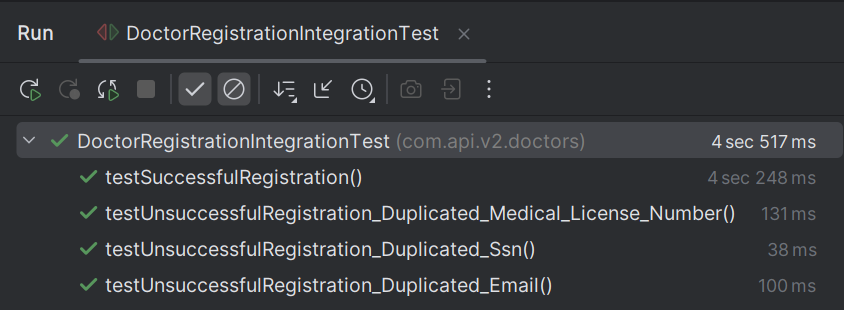
\includegraphics[width=1\linewidth]{figures/results_doctor_registration_integration_test.png}
	\\ \footnotesize Source: Author's creation.
	\label{fig:results_doctor_registration_integration_test}
\end{figure}

As expected, all the results of tests were successful. Methods of integration tests are expected to pass, regardless of successful or unsuccessful representation of the endpoint's response, due to the fact that integration tests are supposed to represent the system's functionality.

\subsection{Doctor Management}

The service \textit{doctorManagementService} manages \textbf{Doctor} by terminating or rehiring them. Therefore, it relies on 2 methods: \textit{terminate()} and \textit{rehire()}. They are handled in the subsections \ref{subsection:doctor_termination} and \ref{subsection:doctor_rehiring}, respectively. In addition, the subsection \ref{subsection:doctor_not_found} applies to both subsections \ref{subsection:doctor_termination} and \ref{subsection:doctor_rehiring} as it verifies if the provided medical license number is associated with an existing \textbf{Doctor}.

\subsubsection{Error Handling: Doctor Not Found}
\label{subsection:doctor_not_found}

The figure \ref{fig:doctor_not_found_activity_diagram} represents an activity diagram that expresses how the server reacts when the provided medical license number is not associated with an existing \textbf{Doctor}.

\begin{figure}[H]
	\centering
	\caption{Flow of Retrieving a Medical Slot}
	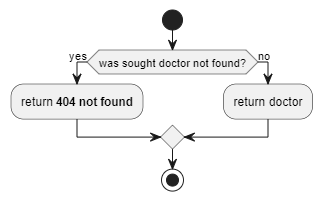
\includegraphics[width=1\linewidth]{figures/doctor_not_found_activity_diagram.png}
	\\ \footnotesize Source: Author's creation.
	\label{fig:doctor_not_found_activity_diagram}
\end{figure}

The retrieval of a \textbf{Doctor} is performed by a utility class. As visibly exposed, if no association between the provided medical license number and an existing \textbf{Doctor} is discovered, the \hyperref[appendix:glossary]{status code 404} is returned. Conversely, the existing \textbf{Doctor} is returned.

\subsubsection{Audit Trail Process}
\label{subsection:doctor_audit_trail} 

This subsection applies to subsections \ref{subsection:doctor_termination} and \ref{subsection:doctor_rehiring}. To ensure data integrity and prevent misrepresentation during these transformations, a shared intermediate process is implemented. This process records the previous state of the \textbf{Doctor
}'s data in the database before any changes are applied. By preserving the prior state, it is possible to maintain an accurate audit trail, enabling transparency, accountability, and compliance with regulatory requirements.

The figure \ref{fig:audit_trail_activity_diagram} represents the activity diagram that presents the flow of recording an audit trail of a \textbf{Doctor}.

\begin{figure}[H]
	\centering
	\caption{Audit Trail Activity Diagram}
	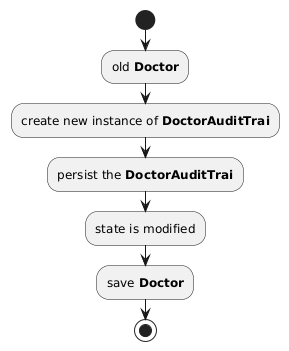
\includegraphics[width=0.5\linewidth]{figures/doctor_audit_trail_activity_diagram.png}
	\label{fig:audit_trail_activity_diagram}
	\\ \footnotesize Source: Author's creation.
\end{figure}

As stated by the figure \ref{fig:audit_trail_activity_diagram}, the current version of \textbf{Doctor} is retrieved and added to the new instance of \textbf{DoctorAuditTrail}. The next step is persisting the new instance of \textbf{DoctorAuditTrail}. After this, the state of \textbf{Doctor} is modified, following the subsections \ref{subsection:doctor_termination} and \ref{subsection:doctor_rehiring}, which creates the new version of \textbf{Doctor}.

\subsubsection{Termination Case}
\label{subsection:doctor_termination}

The process of terminating a \textbf{Doctor} involves the verification performed by the subsection \ref{subsection:doctor_not_found} and if the sought \textbf{Doctor} is currently terminated. If so, the operations shall be handled by an exception. Otherwise, the default behavior is the termination. Thus, the figure \ref{fig:doctor_termination_sequence_diagram} contains the sequence diagram for terminating a Medical Slot.

\begin{figure}[H]
	\centering
	\caption{Doctor Termination Sequence Diagram}
	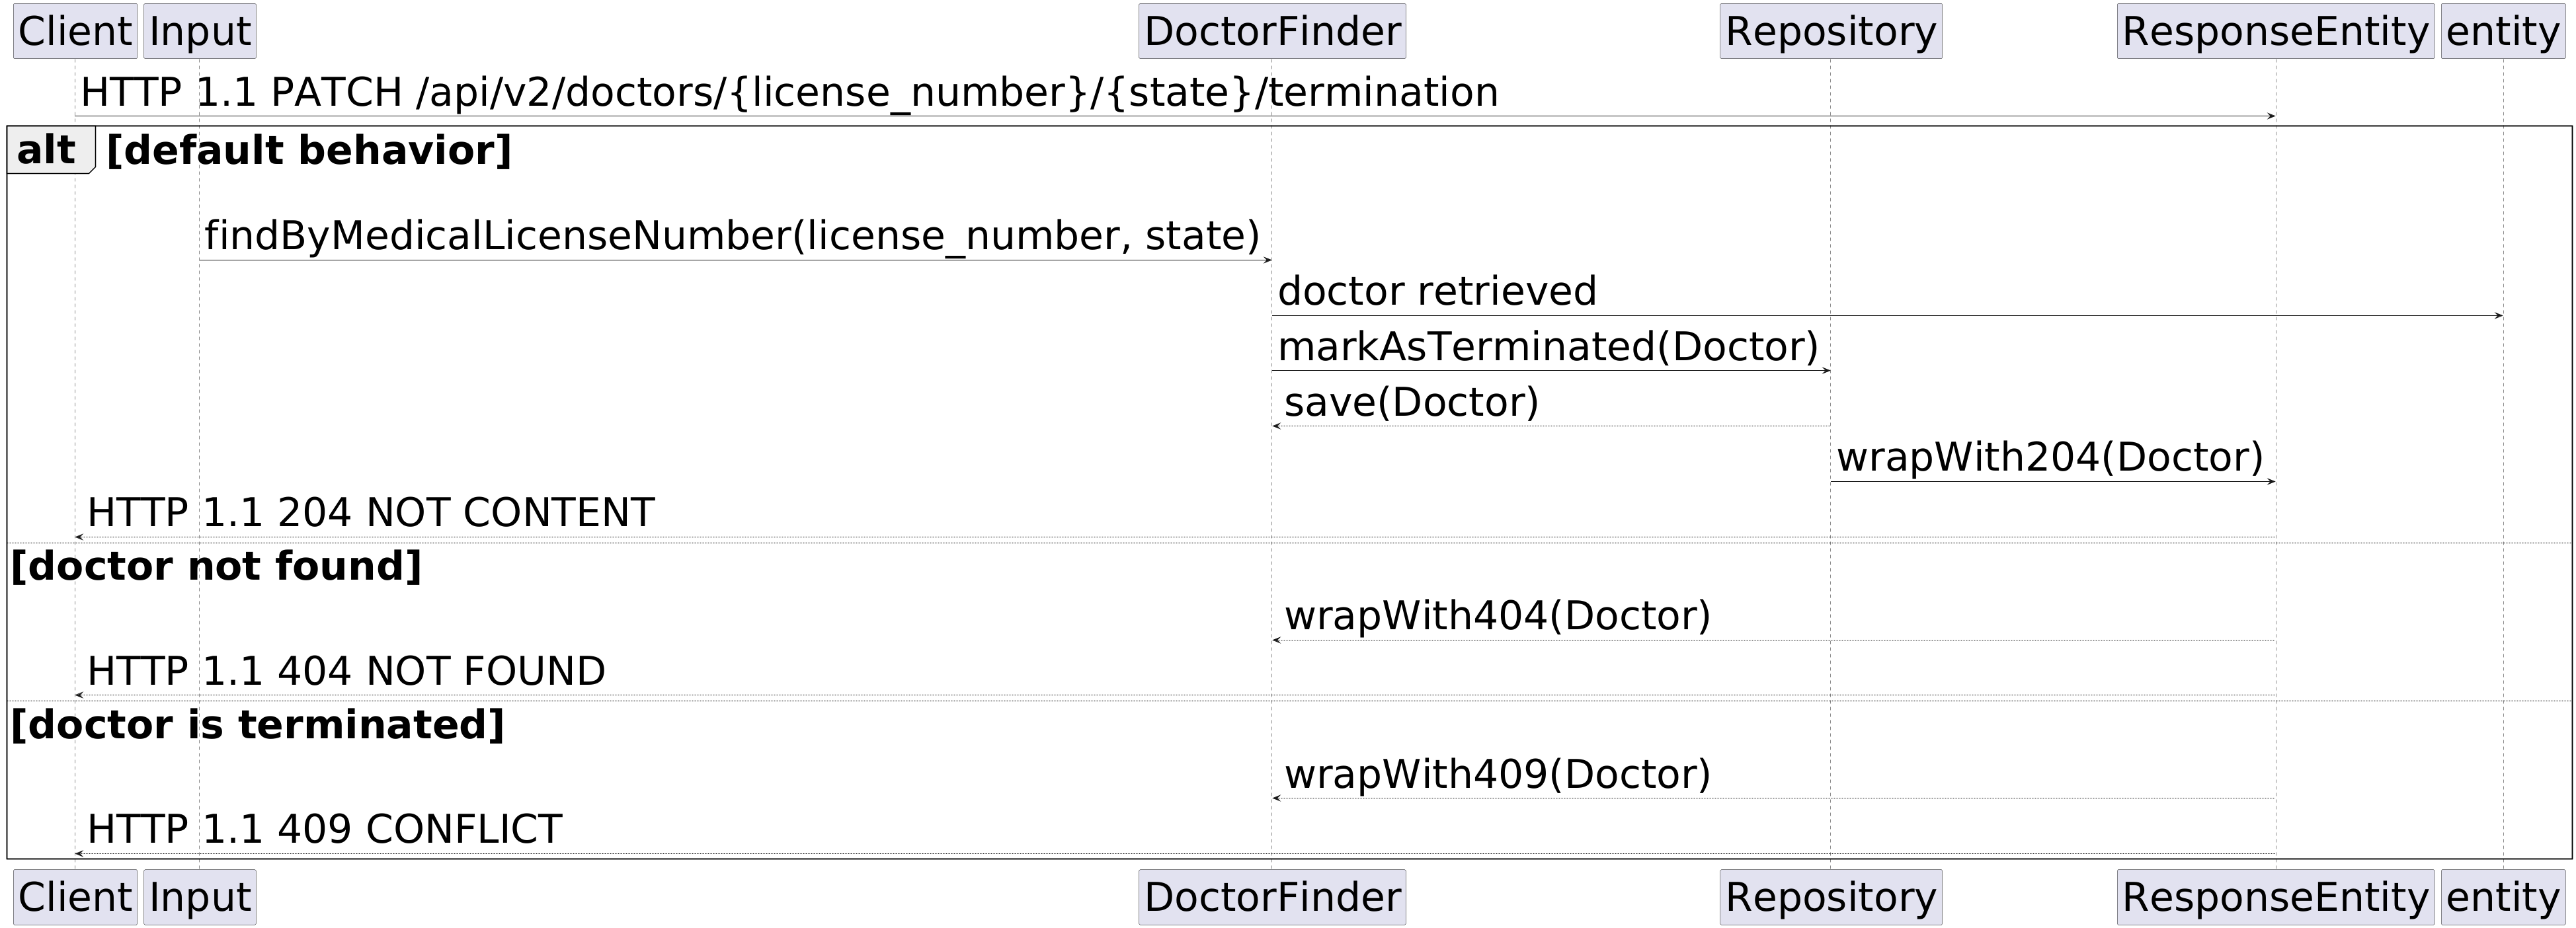
\includegraphics[width=1\linewidth]{figures/doctor_termination_sequence_diagram.png}
	\\ \footnotesize Source: Author's creation.
	\label{fig:doctor_termination_sequence_diagram}
\end{figure}

When the retrieved doctor is currently terminated, the \hyperref[appendix:glossary]{status code 409} is returned. 

The figure \ref{fig:doctor_termination_unsuccessful_integration_test_terminated_doctor} exposes the content of the method \textit{testUnsuccessfulTermination\_Terminated\_Doctor}.

\begin{figure}[H]
	\centering
	\caption{Doctor Termination Unsuccessful Case: Currently Terminated Doctor}
	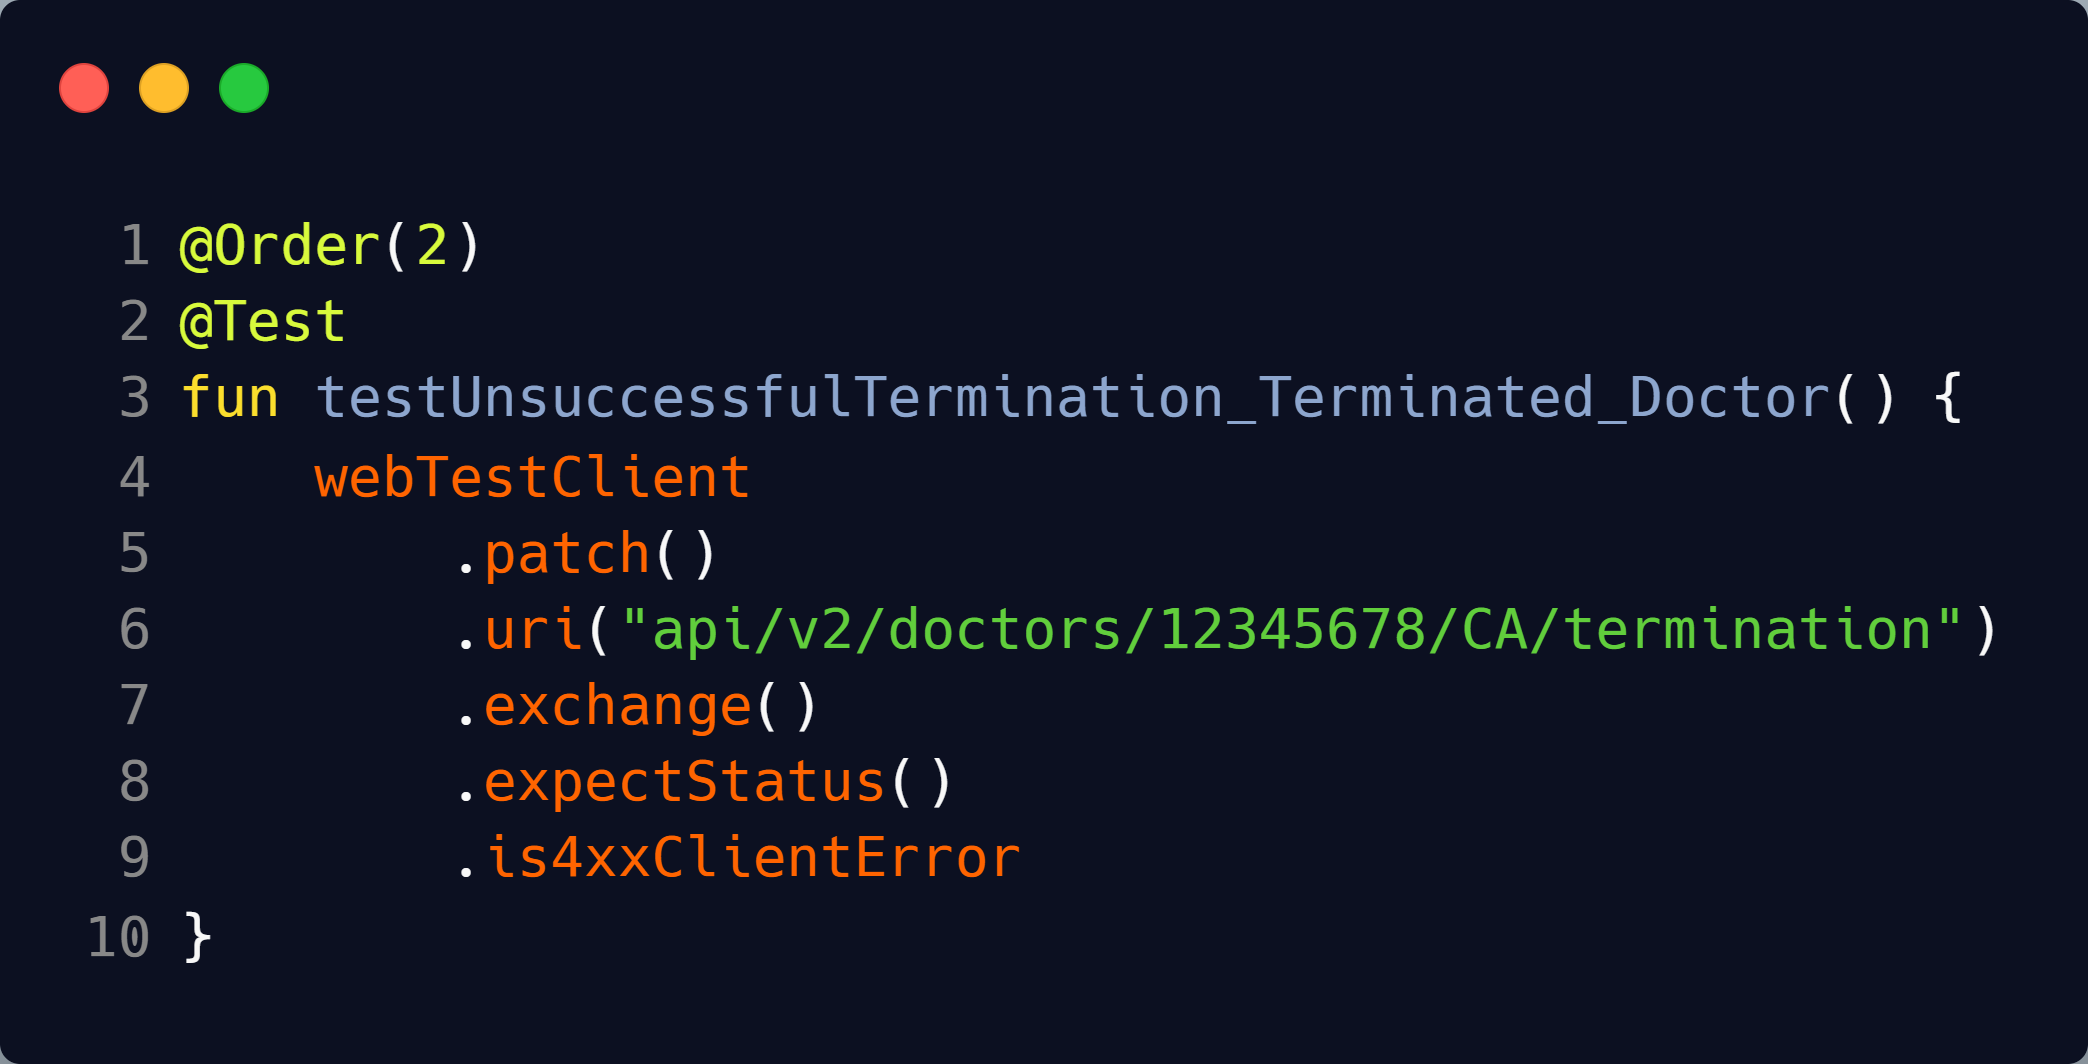
\includegraphics[width=1\linewidth]{figures/doctor_termination_unsuccessful_integration_test_terminated_doctor.png}
	\\ \footnotesize Source: Author's creation.
	\label{fig:doctor_termination_unsuccessful_integration_test_terminated_doctor}
\end{figure}

The method \textit{testUnsuccessfulTermination\_Terminated\_Doctor} uses an instance of the \textit{WebTestClient}, as argued by the \hyperref[subsection:automated_software_testing]{subsection Automated Software Testing}. When, at the moment that validated input data is extracted from the path variables \textit{license\_number} and \textit{state}, the existing \textbf{Doctor} is retrieved. If it is found to be currently terminated, the \hyperref[tab:summary_http_status_codes]{status code 409} is returned.

Otherwise, when the retrieved doctor is currently active, the \hyperref[appendix:glossary]{status code 204} is returned. 

The figure \ref{fig:doctor_termination_successful_integration_test} exposes the content of the method \textit{testSuccessfulTermination}.

\begin{figure}[H]
	\centering
	\caption{Doctor Termination Successful Case}
	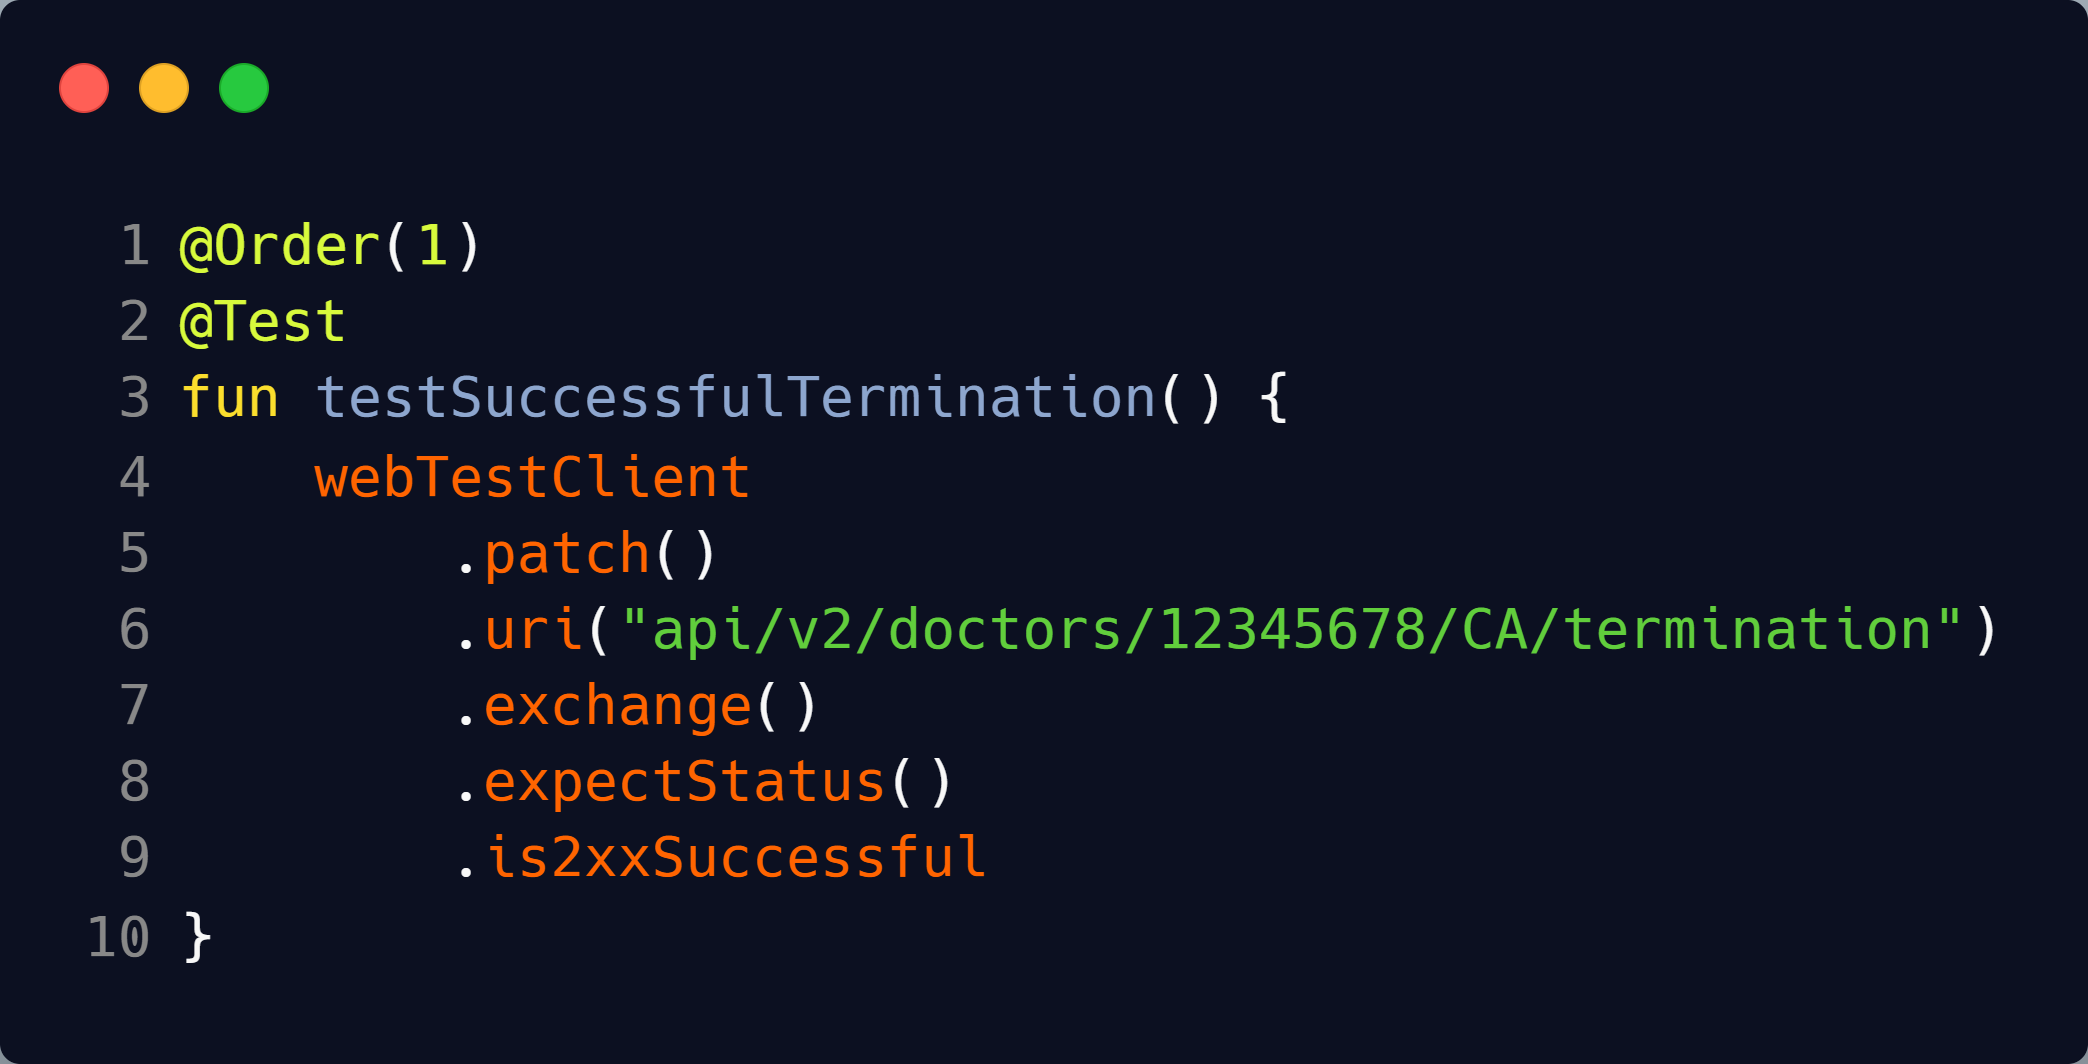
\includegraphics[width=1\linewidth]{figures/doctor_termination_successful_integration_test.png}
	\\ \footnotesize Source: Author's creation.
	\label{fig:doctor_termination_successful_integration_test}
\end{figure}

The method \textit{testSuccessfulRehiring} uses an instance of the \textit{WebTestClient}, as argued by the \hyperref[subsection:automated_software_testing]{subsection Automated Software Testing}. In order to register a \textbf{Doctor}, the PATCH method was used. As clarified by the \hyperref[subsection:http_semantics]{subsection HTTP Semantics}, every HTTP request requires a \hyperref[appendix:glossary]{URI} to route the expected request to the target server aiming to obtain the expected result. Thereby, the \hyperref[appendix:glossary]{URI} \textit{/api/v2/medical\_slots/\underline{license\_number}/\underline{state}/termination} is placed as the argument of \textit{uri()}. Finally, the \hyperref[tab:summary_http_status_codes]{status code 201} is returned.

\subsubsection{Rehiring  Case}
\label{subsection:doctor_rehiring}

The process of rehiring a \textbf{Doctor} involves the verification performed by the subsection \ref{subsection:doctor_not_found} and if the sought \textbf{Doctor} is currently active. If so, the operations shall be handled by an exception. Otherwise, the default behavior is the rehiring. Thus, the figure \ref{fig:doctor_rehiring_sequence_diagram} contains the sequence diagram for terminating a Medical Slot.

\begin{figure}[H]
	\centering
	\caption{Doctor Rehiring Sequence Diagram}
	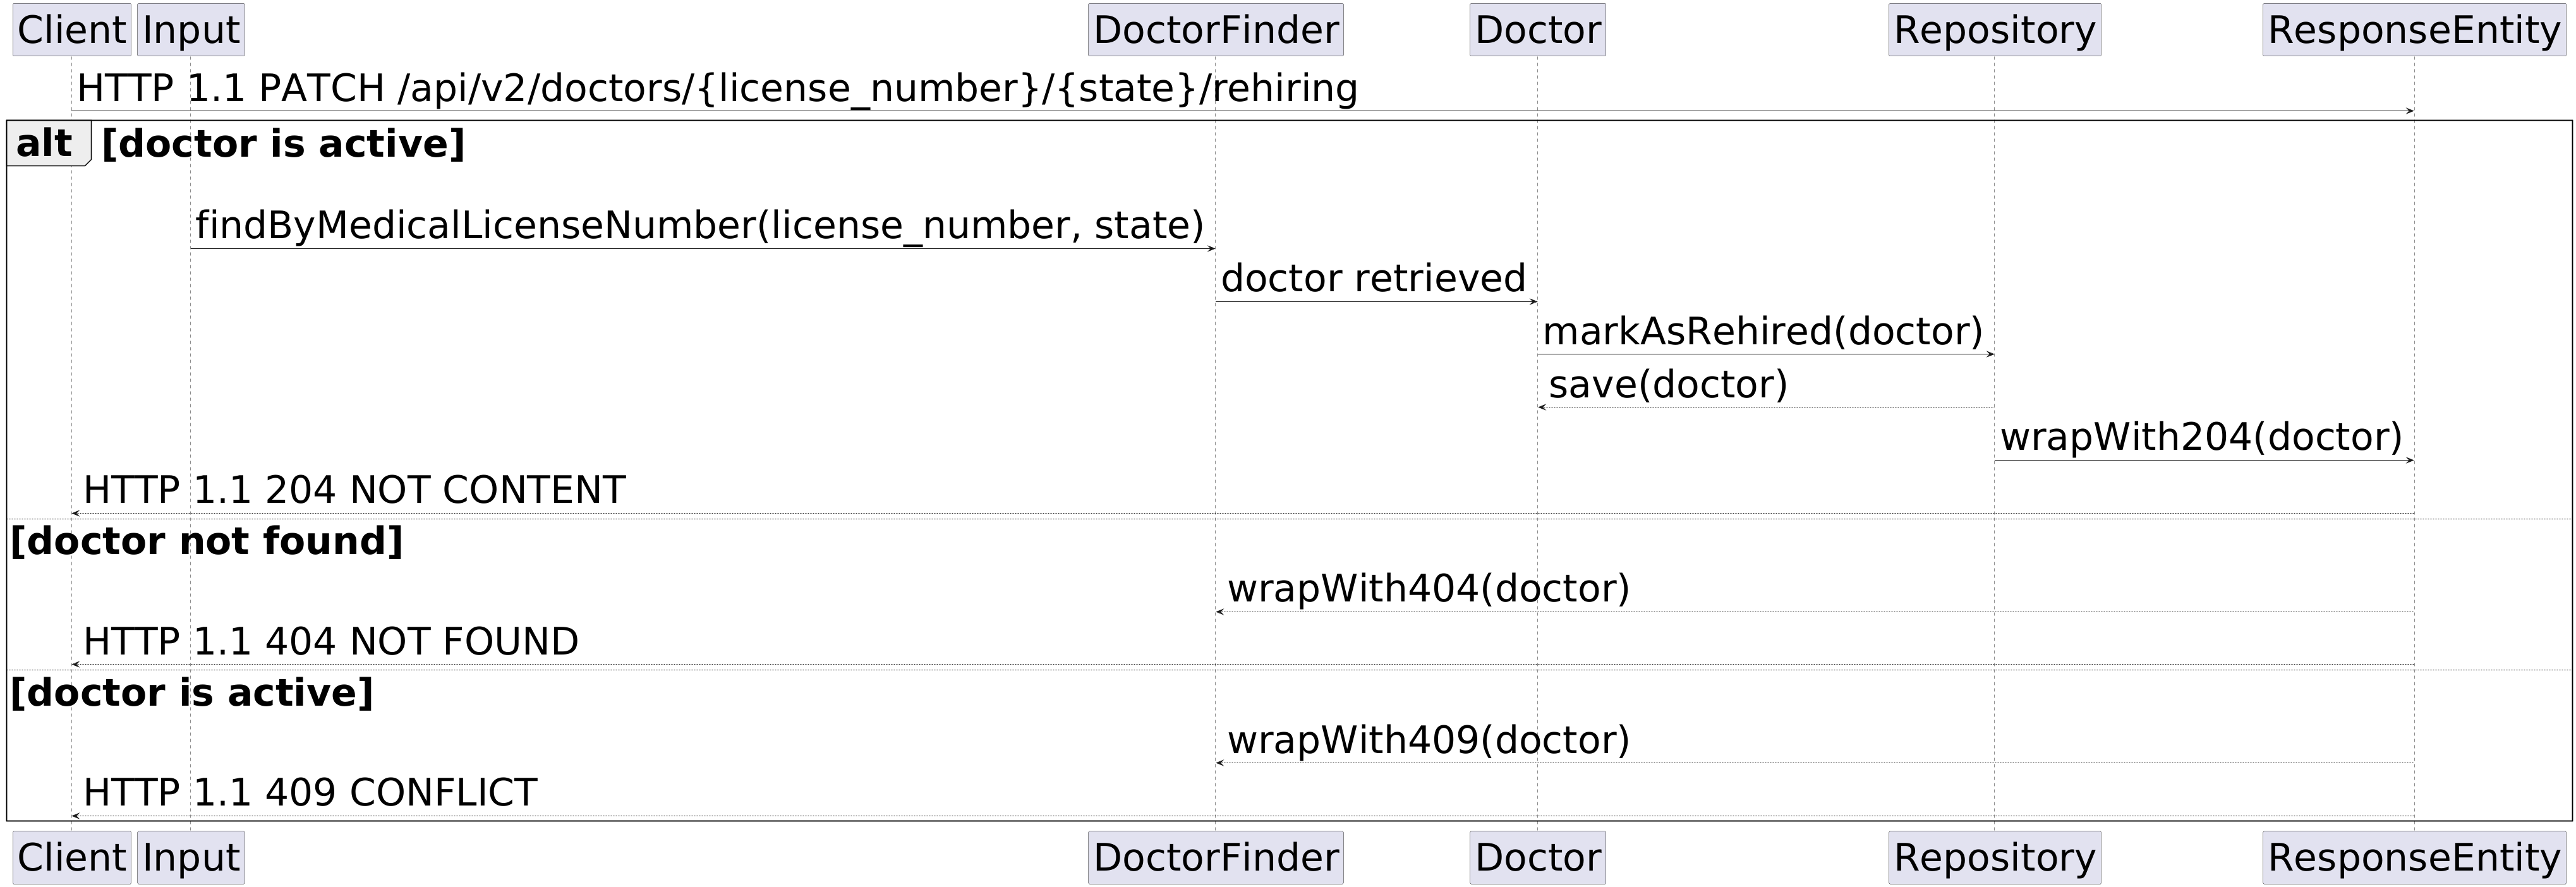
\includegraphics[width=1\linewidth]{figures/doctor_rehiring_sequence_diagram.png}
	\\ \footnotesize Source: Author's creation.
	\label{fig:doctor_rehiring_sequence_diagram}
\end{figure}

When it is discovered that retrieved \textbf{Doctor} is currently active, the \hyperref[tab:summary_http_status_codes]{status code 409} is returned.

The figure \ref{fig:doctor_rehiring_unsuccessful_integration_test_active_doctor} exposes the content of the method \textit{testUnsuccessfulRehiring\_Active\_Doctor}.

\begin{figure}[H]
	\centering
	\caption{Doctor Rehiring Unsuccessful Case: Currently Active Doctor}
	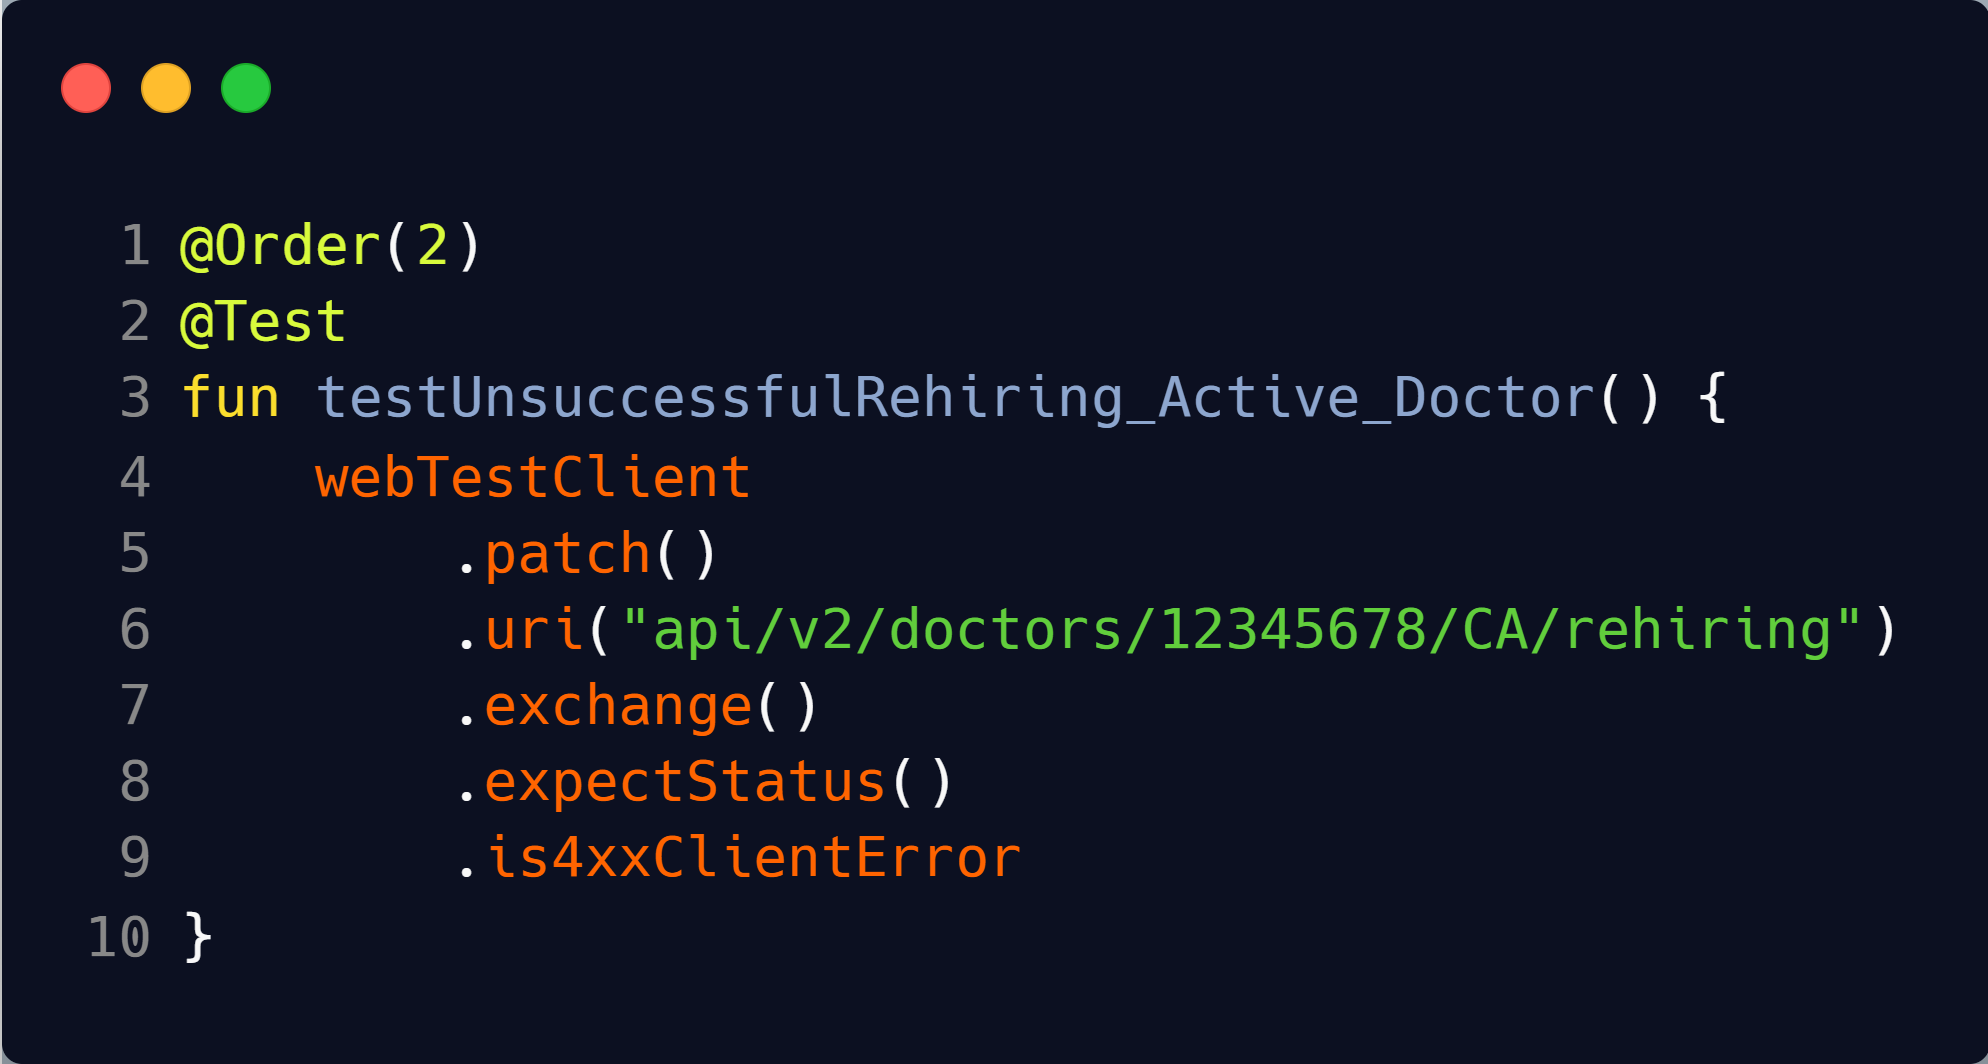
\includegraphics[width=1\linewidth]
	{figures/doctor_rehiring_unsuccessful_integration_test_active_doctor.png}
	\label{fig:doctor_rehiring_unsuccessful_integration_test_active_doctor}
	\footnotesize Source: Author's creation.
\end{figure}

The method \textit{testUnsuccessfulRehirirng\_Active\_Doctor} uses an instance of the \textit{WebTestClient}, as argued by the \hyperref[subsection:automated_software_testing]{subsection Automated Software Testing}. When, at the moment that validated input data is extracted from the path variables \textit{license\_number} and \textit{state}, the existing \textbf{Doctor} is retrieved. If it is found to be currently active, the \hyperref[tab:summary_http_status_codes]{status code 409} is returned.

Otherwise, when it is discovered that retrieved \textbf{Doctor} is currently terminated, the \hyperref[tab:summary_http_status_codes]{status code 204} is returned.

The figure \ref{fig:doctor_rehiring_successful_integration_test} exposes the content of the method \textit{testSuccessfulRehiring}.

\begin{figure}[H]
	\centering
	\caption{Doctor Rehiring Successful Case}
	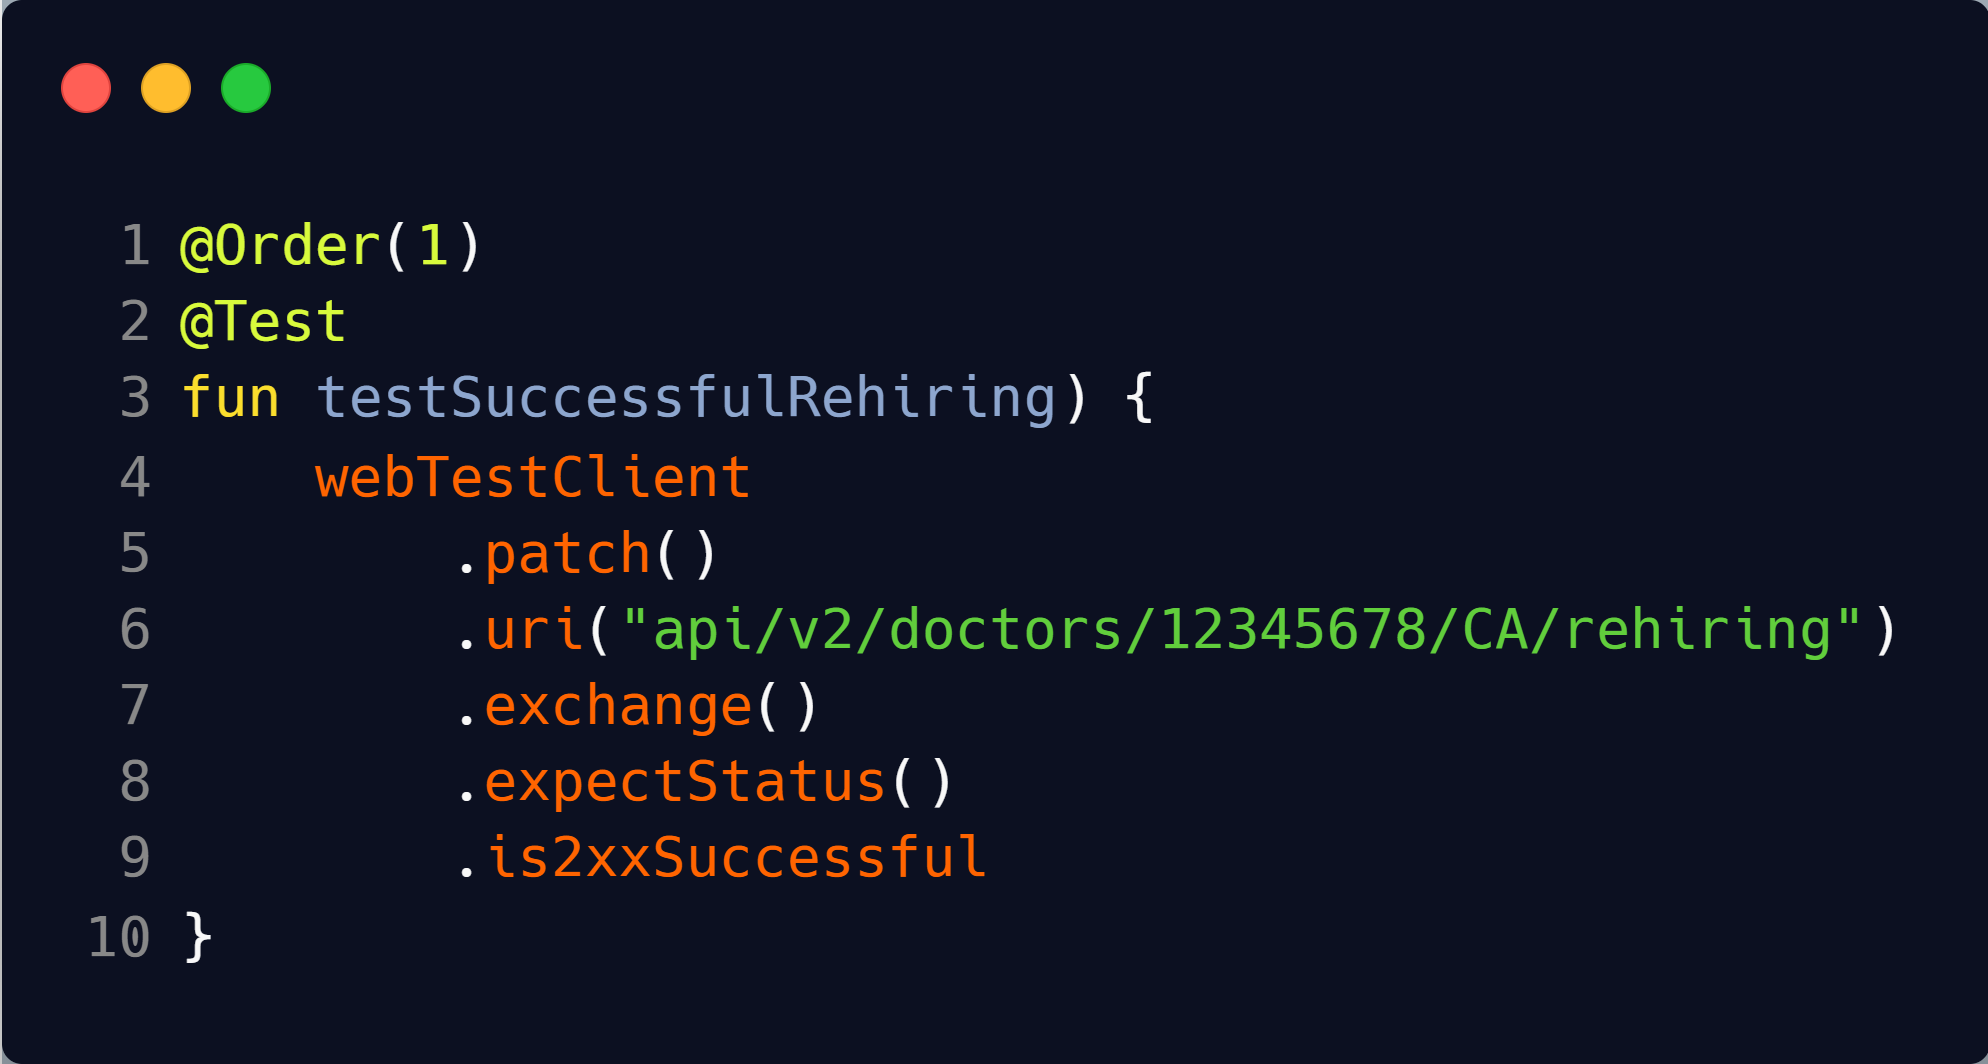
\includegraphics[width=1\linewidth]
	{figures/doctor_rehiring_successful_integration_test.png}
	\label{fig:doctor_rehiring_successful_integration_test}
	\footnotesize Source: Author's creation.
\end{figure}

The method \textit{testSuccessfulRehiring} uses an instance of the \textit{WebTestClient}, as argued by the \hyperref[subsection:automated_software_testing]{subsection Automated Software Testing}. In order to register a \textbf{Doctor}, the PATCH method was used. As clarified by the \hyperref[subsection:http_semantics]{subsection HTTP Semantics}, every HTTP request requires a \hyperref[appendix:glossary]{URI} to route the expected request to the target server aiming to obtain the expected result. Thereby, the \hyperref[appendix:glossary]{URI} \textit{/api/v2/medical\_slots/\underline{license\_number}/\underline{state}/rehiring} is placed as the argument of \textit{uri()}. Finally, the \hyperref[tab:summary_http_status_codes]{status code 201} is returned.

\subsubsection{Summary of Results}

\begin{figure}[H]
	\centering
	\caption{Doctor Termination Integration Test's Results}
	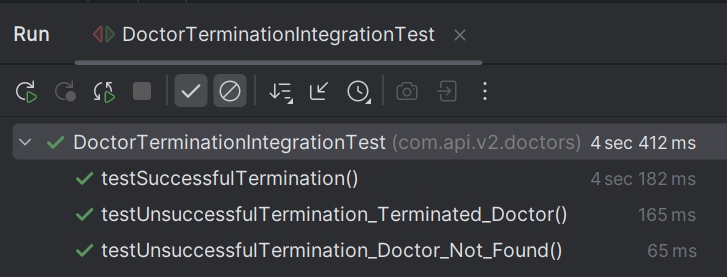
\includegraphics[width=1\linewidth]{figures/results_doctor_termination_integration_test.PNG}
	\label{fig:results_doctor_termination_integration_test}
	\footnotesize Source: Author's creation.
\end{figure}

\begin{figure}[H]
	\centering
	\caption{Doctor Rehiring Integration Test's Results}
	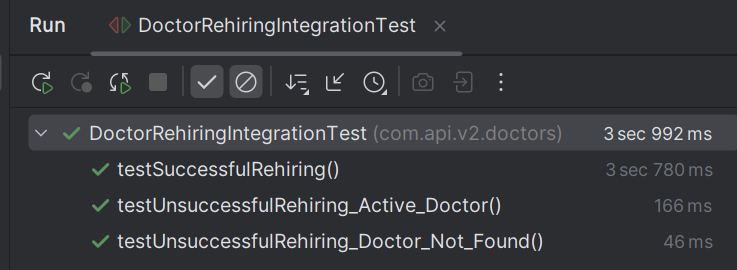
\includegraphics[width=1\linewidth]{figures/results_doctor_rehirirng_integration_test.PNG}
	\label{fig:results_doctor_rehirirng_integration_test}
	\footnotesize Source: Author's creation.
\end{figure}

As expected, all the results of tests were successful. Methods of integration tests are expected to pass, regardless of the successful or unsuccessful representation of the endpoint's response, due to the fact that integration tests are supposed to represent the system's functionality.

\subsection{Medical Slot Registration}

The figure \ref{fig:medical_slot_registration_activity_diagra} embodies the flow of registering a medical slot.

\begin{figure}[H]
	\centering
	\caption{Flow of Registering A Medical Slot}
	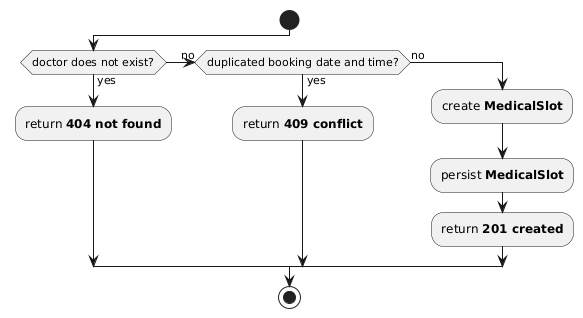
\includegraphics[width=1\linewidth]{figures/medical_slot_registration_activity_diagram.png}
	\label{fig:medical_slot_registration_activity_diagra}
	\footnotesize Source: Author's creation.
\end{figure}

When the sought \textbf{Doctor} was not found, what the subsection \ref{subsection:doctor_not_found}. When the provided booking date and time are currently associated with an active \textbf{Medical Slot} with the found \textbf{Doctor}, the \hyperref[appendix:glossary]{status code 404} is returned. Additionally, the \hyperref[appendix:glossary]{status code 409} is the output when the provided booking date and time are currently in use with an active \textbf{Medical Slot} whose doctor is sought \textbf{Doctor}. Contrarily, an instance of \textbf{MedicalSlot} is created and persisted. Finally, the \hyperref[tab:summary_http_status_codes]{status code 201} is returned.

The more detailed representation of the registration of a \textbf{MedicalSlot} is represented in the sequence diagram (figure \ref{fig:medical_slot_registration_sequence_diagram}).

\begin{figure}[H]
	\centering
	\caption{Medical Slot Registration Sequence Diagram}
	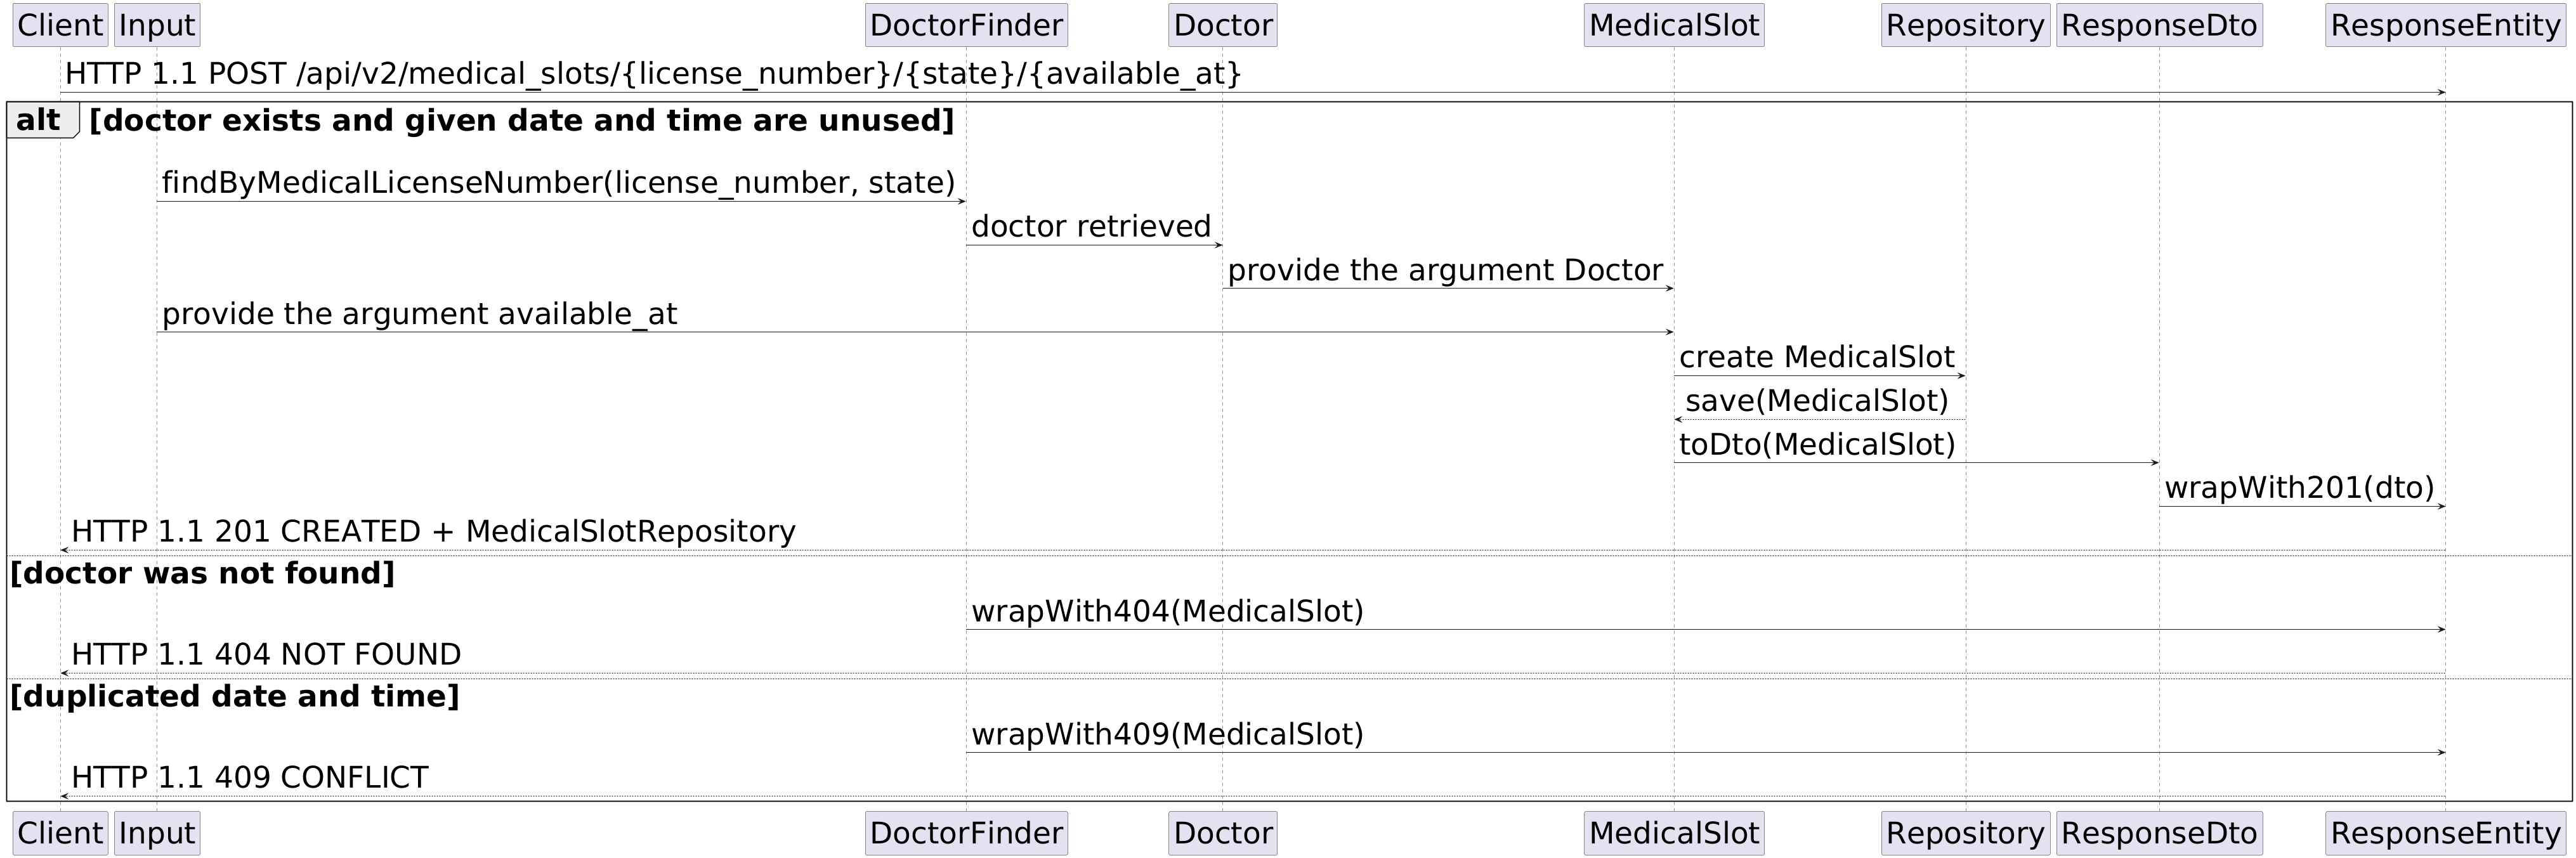
\includegraphics[width=1\linewidth]{figures/medical_slot_registration_sequence_diagram.png}
	\label{fig:medical_slot_registration_sequence_diagram}
	\footnotesize Source: Author's creation.
\end{figure}

The client, whose behavior is described in the \hyperref[subsection:http_semantics]{subsection HTTP Semantics}, requests a resource. It uses the \hyperref[appendix:glossary]{URI} \textit{/api/v2/medical\_slots/\underline{license\_number}/\underline{state}/\underline{available\_at}}. The \hyperref[appendix:glossary]{URI} follows the pattern established  in the table \ref{tab:http-server-schemes}.

The path variables \textit{license\_number}, \textit{state}, and \textit{available\_at} are passed, respectively, to the \hyperref[appendix:glossary]{URI} \textit{/api/v2/medical\_slots/\underline{license\_number}/\underline{state}/\underline{available\_at}} as arguments. The service creates a new \textbf{MedicalSlot}, then persists it.

As exposed by the figure \ref{fig:medical_slot_registration_sequence_diagram}, the sought \textbf{Doctor} is retrieved by the utility class \textbf{DoctorFinder}. If the outcome is null, the \hyperref[tab:summary_http_status_codes]{status code 404} is returned  with the exception \textit{NonExistentDoctorException}; otherwise, the sought \textbf{Doctor} is returned. 
Although, when the provided booking date and time are currently in use with a \textbf{MedicalSlot} whose doctor is the sought \textbf{Doctor}, the \hyperref[tab:summary_http_status_codes]{status code 409} is returned with the exception \textit{UnavailableBookingDateTimeException}. As the default behavior, with \textbf{Doctor} and \textit{available\_at}, the new \textbf{MedicalSlot} is created, persisted, turned into a \hyperref[appendix:glossary]{DTO}, and wrapped in the \hyperref[tab:summary_http_status_codes]{status code 201}.

\subsubsection{Successful Case}

\begin{figure}[H]
	\centering
	\caption{Medical Slot Registration Successful Case}
	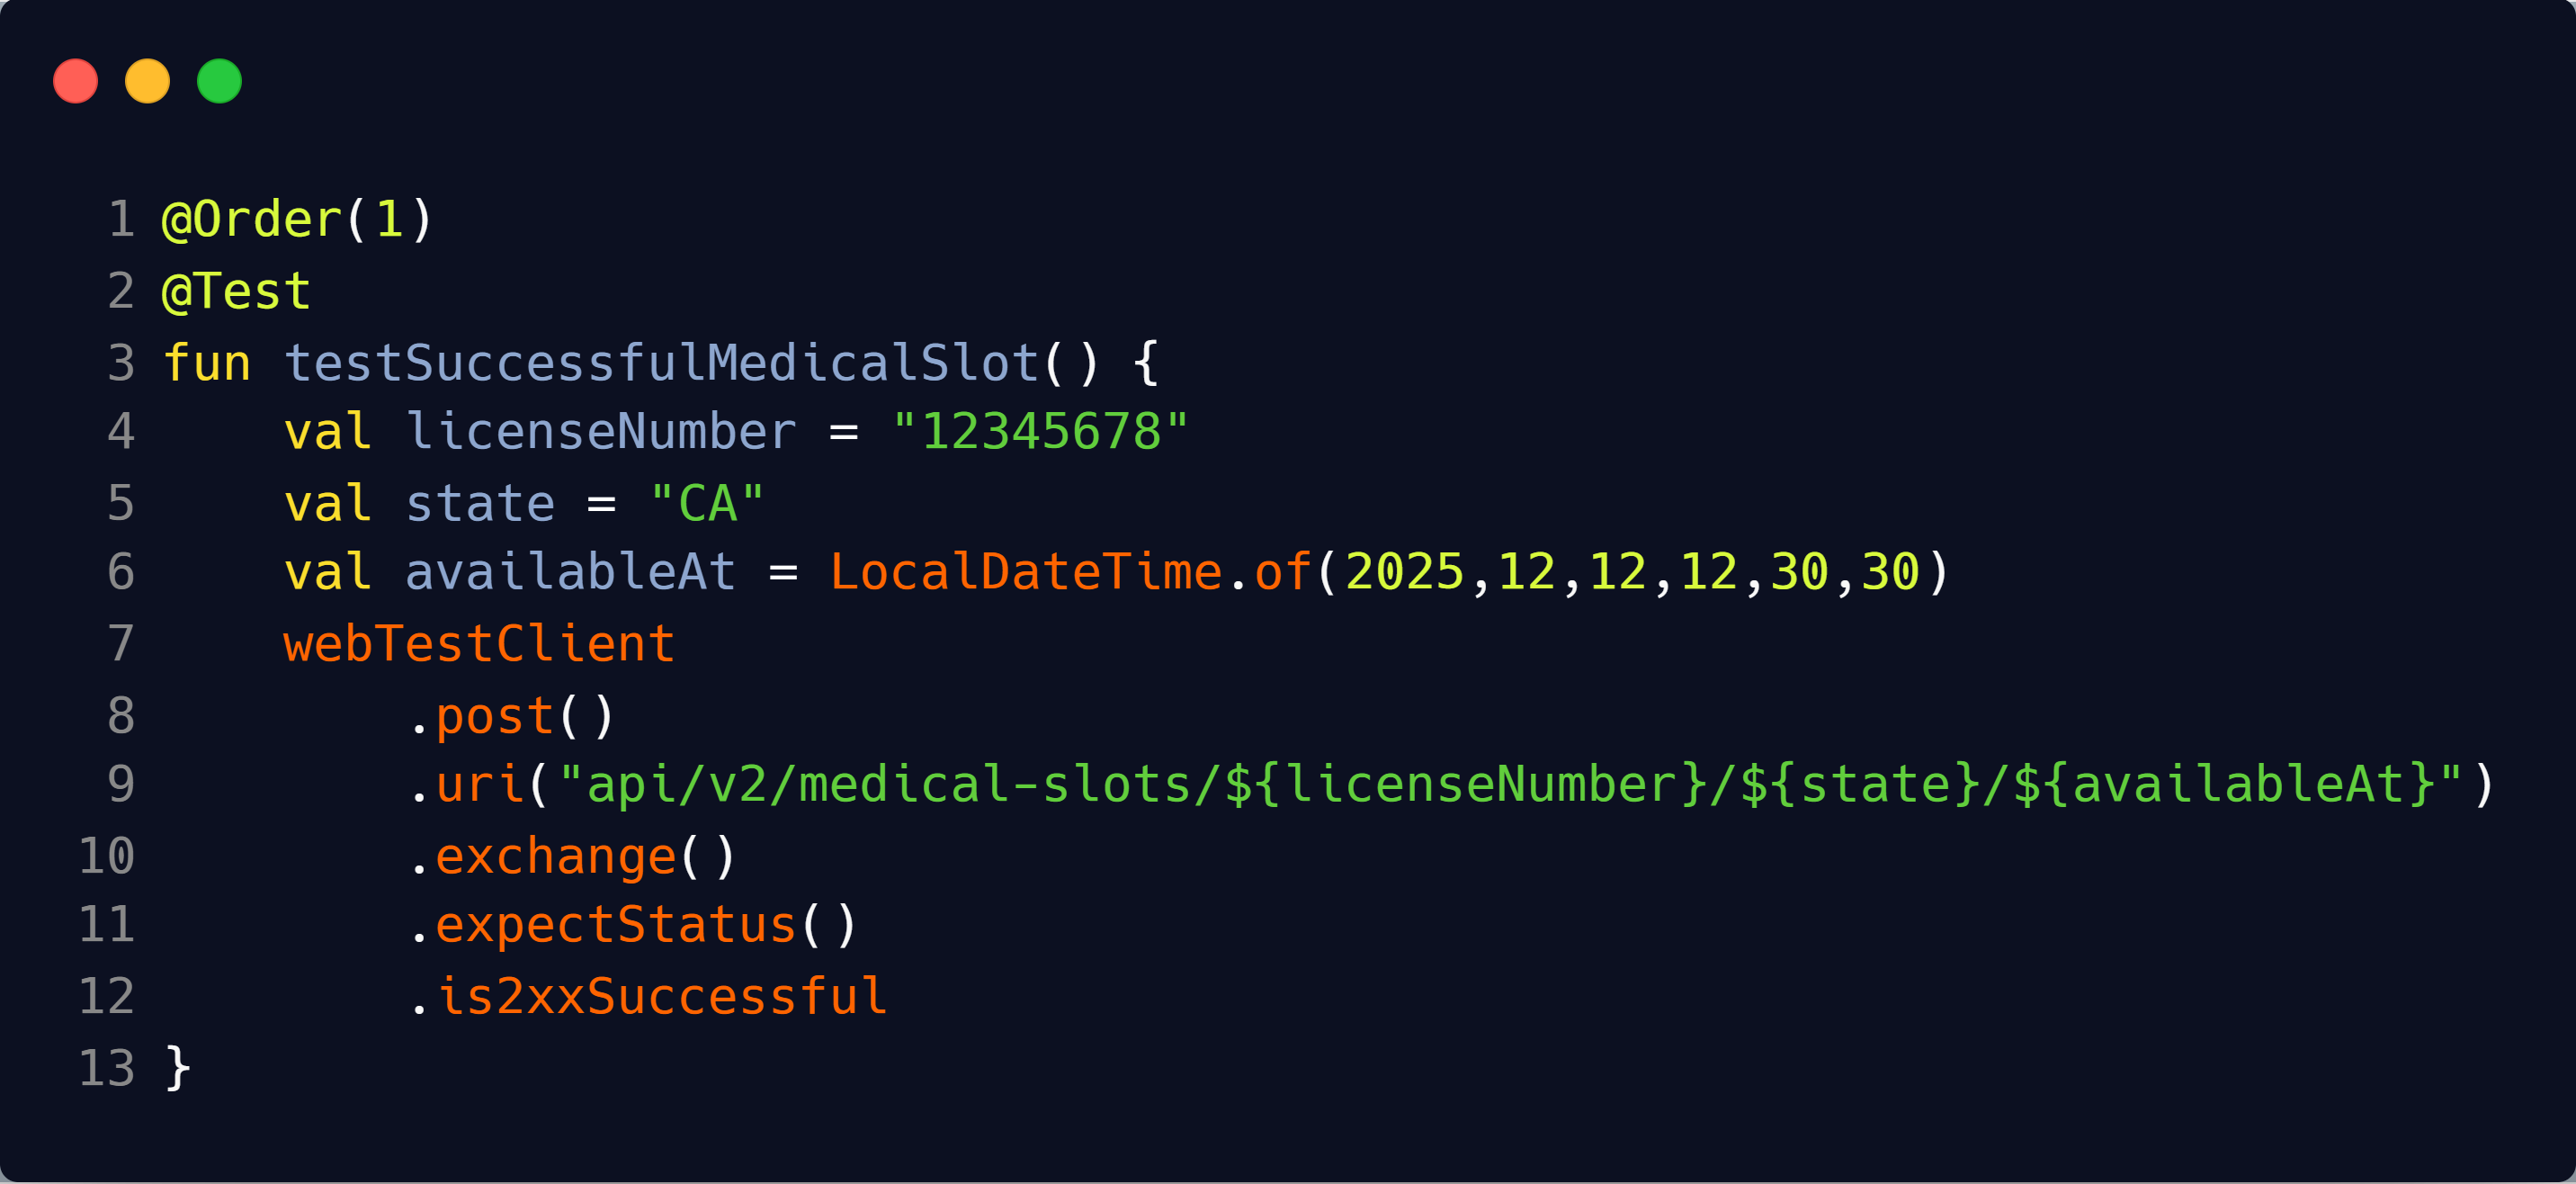
\includegraphics[width=1\linewidth]{figures/medical_slot_registration_successful_integration_test.png}
	\label{fig:medical_slot_registration_successful_integration_test}
	\footnotesize Source: Author's creation.
\end{figure}

The method \textit{testSuccessfulRegistration} uses an instance of the \textit{WebTestClient}, as argued by the \hyperref[subsection:automated_software_testing]{subsection Automated Software Testing}. In order to register a \textbf{Doctor}, the POST method was used. As clarified by the \hyperref[subsection:http_semantics]{subsection HTTP Semantics}, every HTTP request requires a \hyperref[appendix:glossary]{URI} to route the expected request to the target server aiming to obtain the expected result. Thereby, the \hyperref[appendix:glossary]{URI} \textit{/api/v2/medical\_slots/\underline{license\_number}/\underline{state}/\underline{available\_at}} is placed as the argument of \textit{uri()}. Finally, the \hyperref[tab:summary_http_status_codes]{status code 201} is returned.

\subsubsection{Unsuccessful Case: Not Found Doctor}

\begin{figure}[H]
	\centering
	\caption{Medical Slot Registration Unsuccessful Case: Doctor Not Found}
	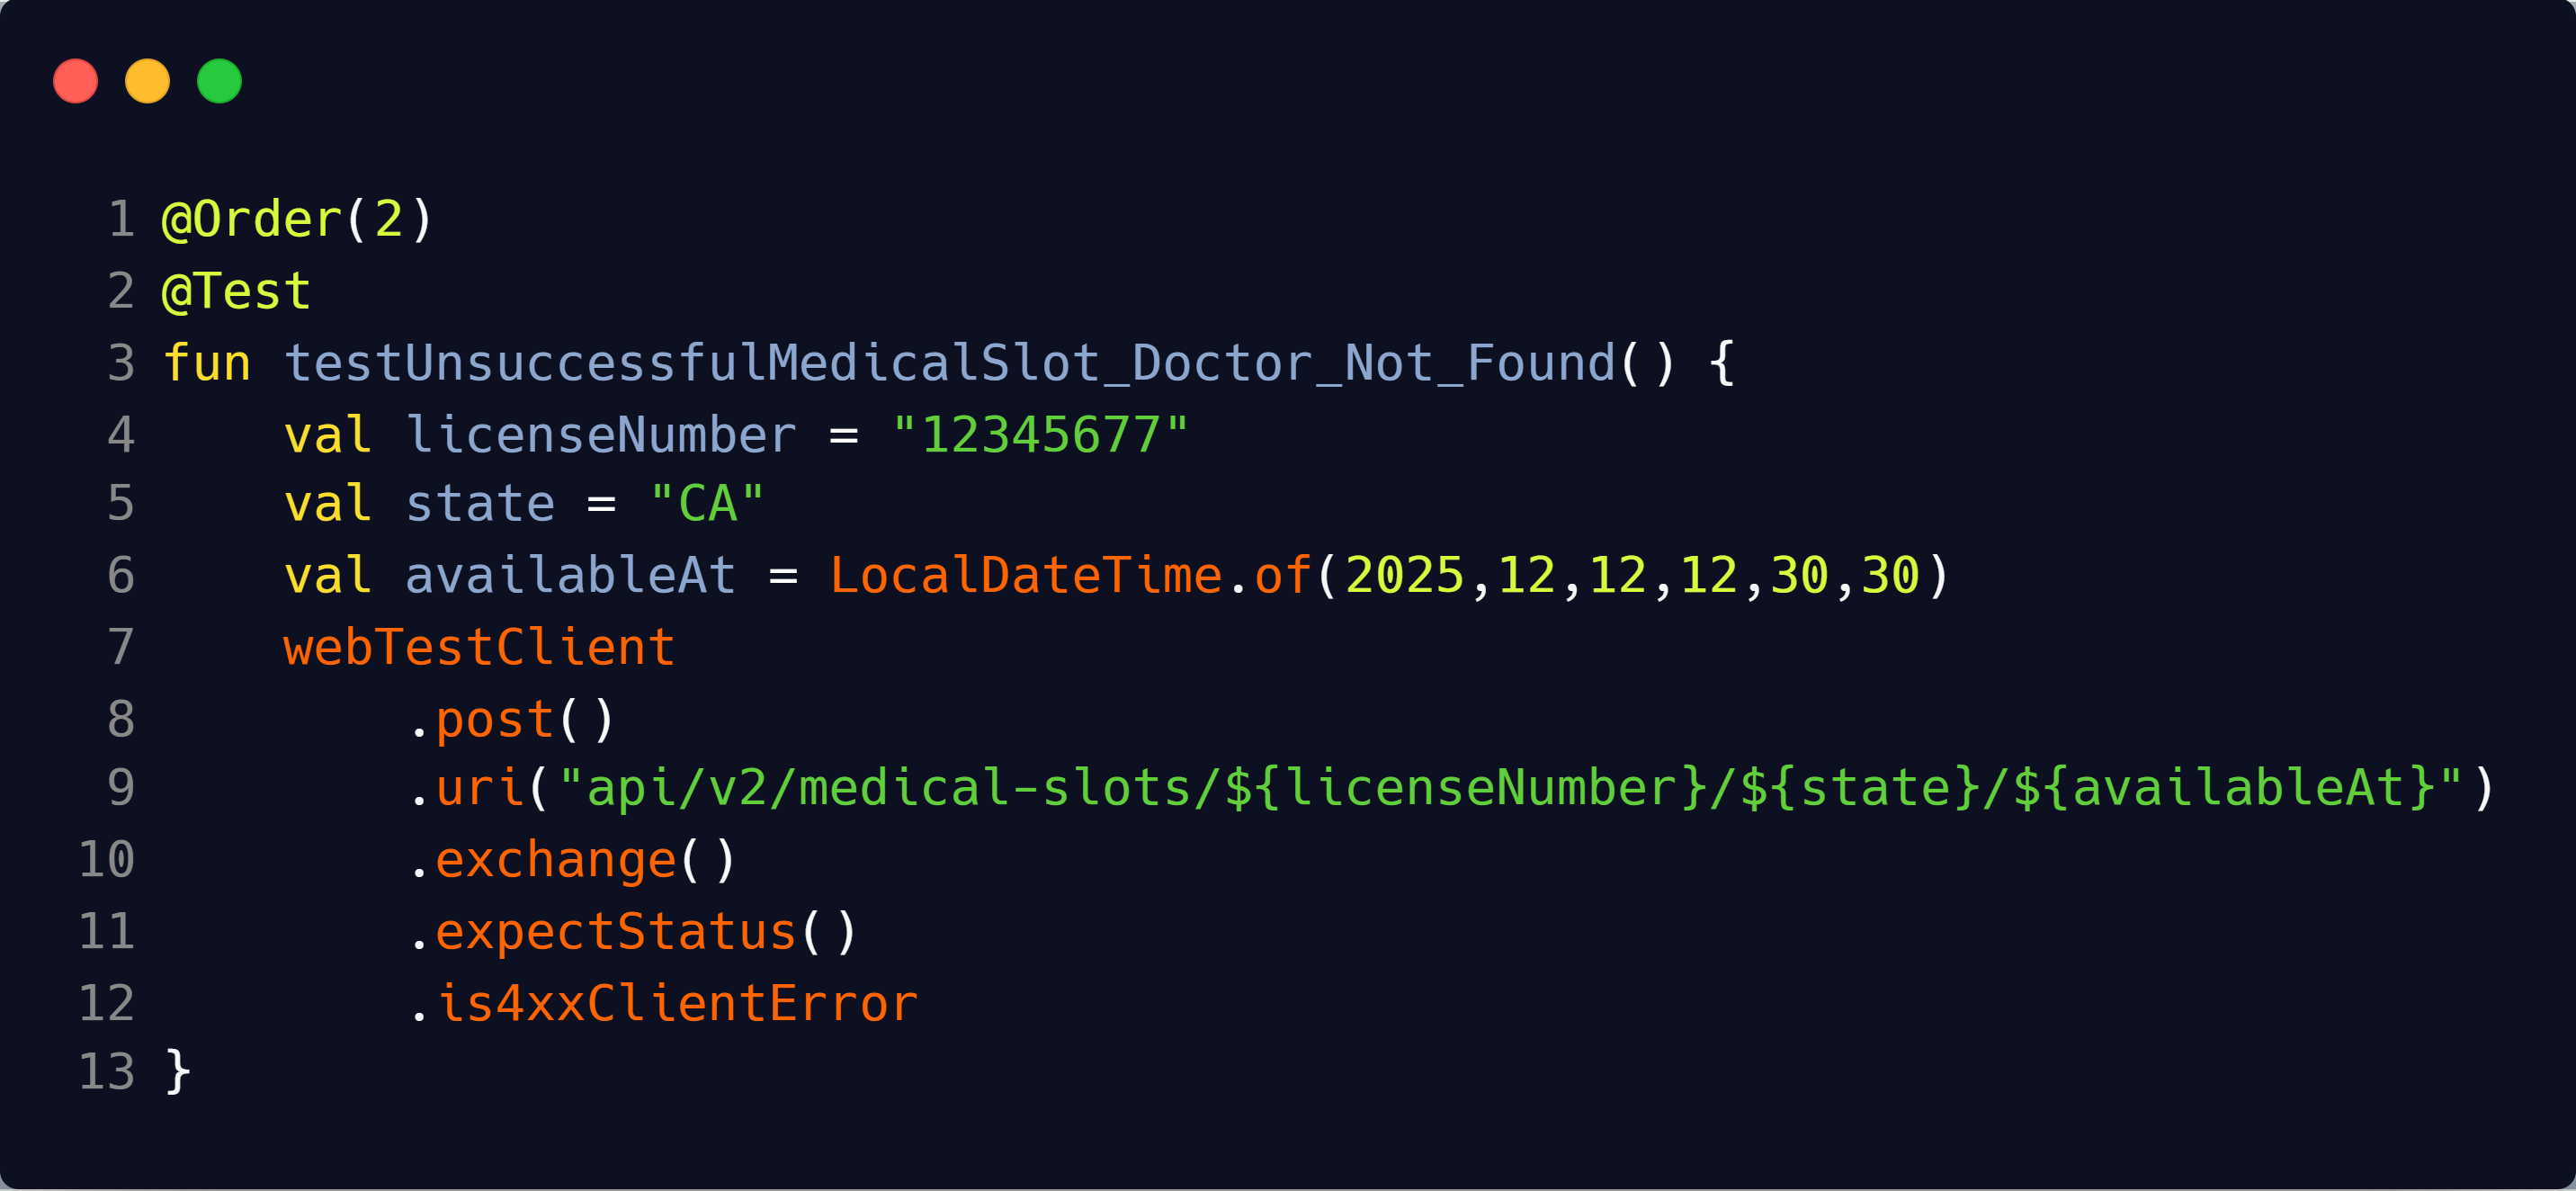
\includegraphics[width=1\linewidth]{figures/medical_slot_registration_unsuccessful_integration_test_doctor_not_found.png}
	\footnotesize Source: Author's creation.
	\label{fig:medical_slot_registration_unsuccessful_integration_test_doctor_not_found}
\end{figure}

The method \textit{testUnsuccessfulRegistration\_Doctor\_Not\_Found} uses an instance of the \textit{WebTestClient}, as argued by the \hyperref[subsection:automated_software_testing]{subsection Automated Software Testing}. When, at the moment that validated input data is extracted from the path variables \textit{license\_number}, \textit{state}, and \textit{available\_at} and it is discovered that the sought \textbf{Doctor} is null, the \hyperref[tab:summary_http_status_codes]{status code 404} is returned.

\subsubsection{Unsuccessful Case: Duplicated Booking Date And Time}

\begin{figure}[H]
	\centering
	\caption{Medical Slot Registration Unsuccessful Case: Duplicated Booking Date And Time}
	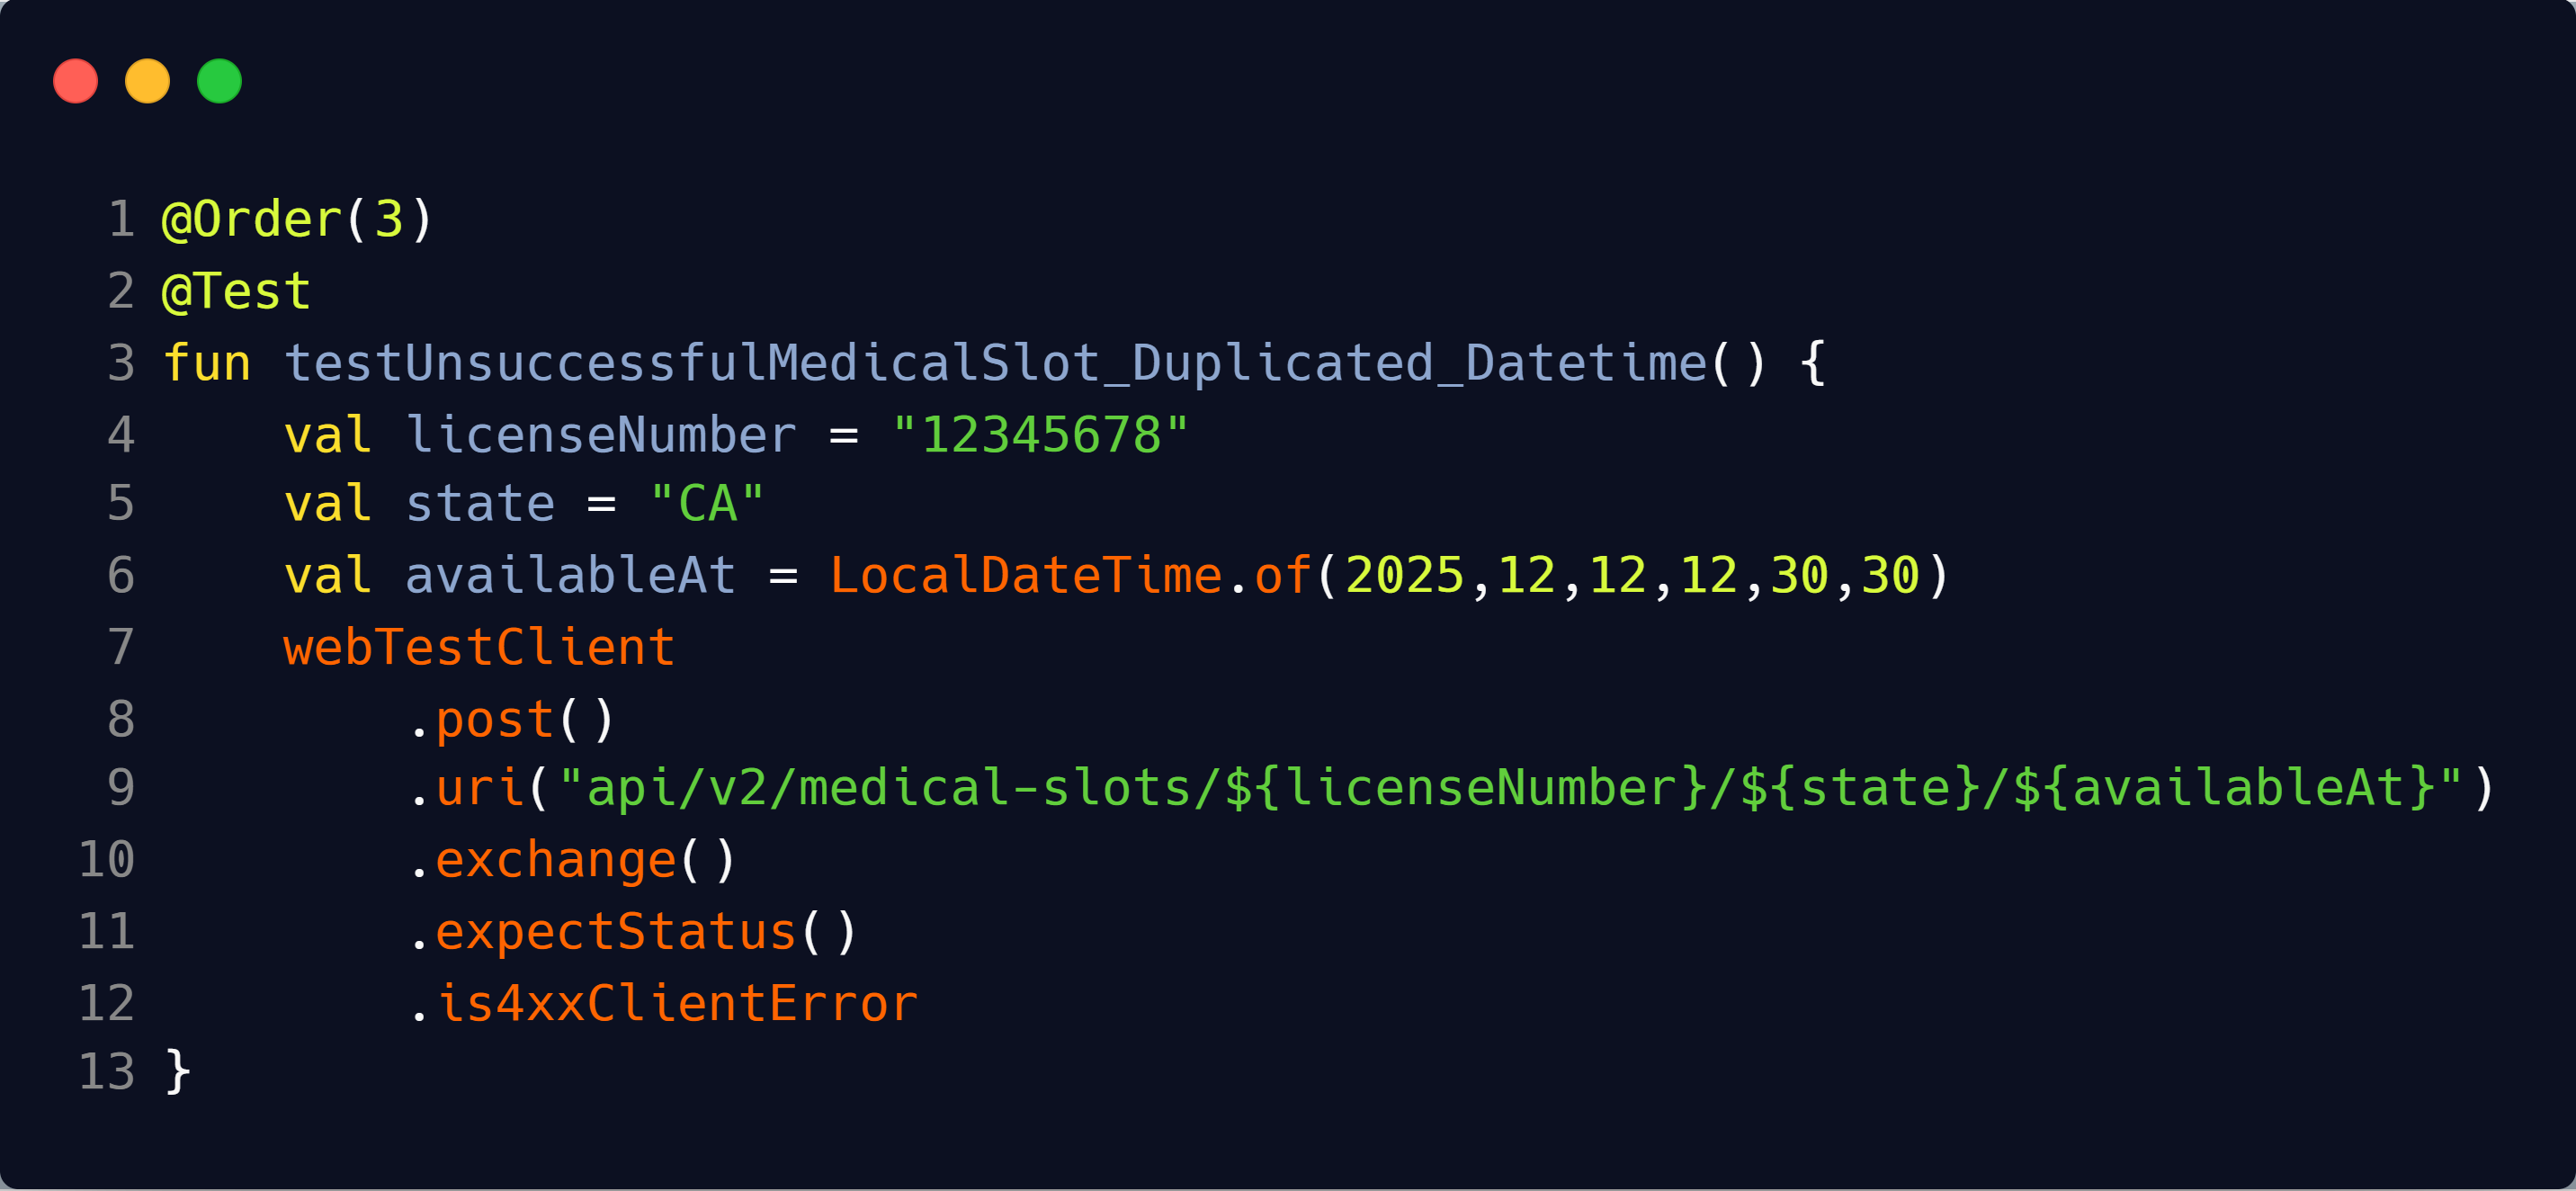
\includegraphics[width=1\linewidth]{figures/medical_slot_registration_unsuccessful_integration_test_duplicated_datetime.png}
	\footnotesize Source: Author's creation.
	\label{fig:medical_slot_registration_unsuccessful_integration_test_duplicated_datetime}
\end{figure}

The method \textit{testUnsuccessfulRegistration\_Duplicated\_Datetime} uses an instance of the \textit{WebTestClient}, as argued by the \hyperref[subsection:automated_software_testing]{subsection Automated Software Testing}. When, at the moment that validated input data is extracted from the path variables \textit{license\_number}, \textit{state}, and \textit{available\_at}, and it is discovered that the provided booking date and time are associated with an active \textbf{MedicalSlot} whose doctor is the sought \textbf{Doctor}, the \hyperref[tab:summary_http_status_codes]{status code 409} is returned.

\subsubsection{Summary of Results}

\begin{figure}[H]
	\centering
	\caption{Medical Slot Registration Integration Test's Results}
	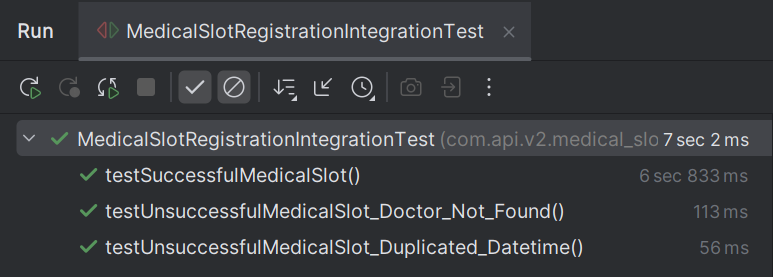
\includegraphics[width=1\linewidth]{figures/results_medical_slot_registration_integration_test.PNG}
	\footnotesize Source: Author's creation.
	\label{fig:results_medical_slot_registration_integration_test}
\end{figure}

As expected, all the results of tests were successful. Methods of integration tests are expected to pass, regardless of the successful or unsuccessful representation of the endpoint's response, due to the fact that integration tests are supposed to represent the system's functionality.

\subsection{Medical Slot Management}

The management of \textbf{MedicalSlot} is divided into methods: \textit{cancel()} and \textit{complete()}. They both share the validations: not found doctor, currently canceled or completed medical slot. The subsections \hyperref[subsection:doctor_not_found]{Error Handling: Doctor Not Found}, \ref{subsection:canceled_or_completed_medical_slot} and apply to the subsections \ref{subsection:medical_slot_cancellation} and \ref{subsection:medical_slot_completion}.

\subsubsection{Error Handling: Currently Canceled or Completed Medical Slot}
\label{subsection:canceled_or_completed_medical_slot}

\begin{figure}[H]
	\centering
	\caption{Canceled or Completed Medical Slot Flow}	
	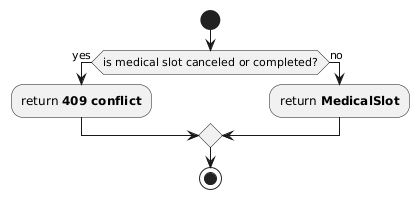
\includegraphics[width=1\linewidth]{figures/medical_slot_canceled_or_completed_activity_diagram.png}
		\footnotesize Source: Author's creation.
		\label{fig:subsection:canceled_or_completed_medical_slot}
\end{figure}

When the sought \textbf{MedicalSlot} is either canceled or completed, the \hyperref[tab:summary_http_status_codes]{status code 409} is returned. Otherwise, the currently active \textbf{MedicalSlot} is returned.

\subsubsection{Cancellation Process}
\label{subsection:medical_slot_cancellation}

\subsubsection{Completion Process}
\label{subsection:medical_slot_completion}

\subsubsection{Summary of Results}

As expected, all the results of tests were successful. Methods of integration tests are expected to pass, regardless of the successful or unsuccessful representation of the endpoint's response, due to the fact that integration tests are supposed to represent the system's functionality.

\subsection{Medical appointment Registration}

The figure \ref{fig:medical_appointment_registration_activity_diagram} illustrates the flow of registering a medical appointment.

\begin{figure}[H]
	\centering
	\caption{Flow of Registering a Medical Appointment}
	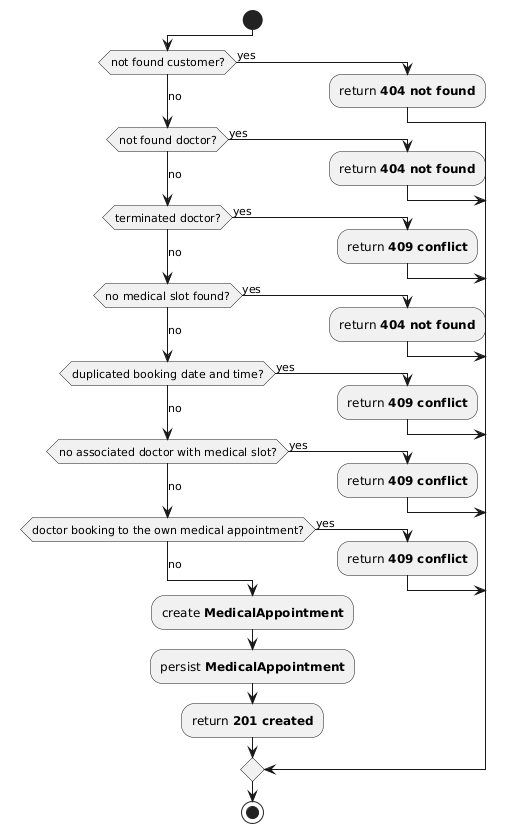
\includegraphics[width=0.6\linewidth]{figures/medical_appointment_registration_activity_diagram.PNG}
	\\ \footnotesize Source: Author's creation.
	\label{fig:medical_appointment_registration_activity_diagram}
\end{figure}

If any of the following--\textbf{Customer}, \textbf{Doctor}, or \textbf{MedicalSlot}--is null,, the \hyperref[tab:summary_http_status_codes]{status code 404} is returned.
Moreover, the \hyperref[tab:summary_http_status_codes]{status code 409} is returned when the provided booking date and time is currently in use with an active medical appointment whose customer is the sought \textbf{Customer} and whose doctor is the sought \textbf{Doctor}. Additionaly,  the \hyperref[tab:summary_http_status_codes]{status code 409} is returned when \textbf{Doctor} is not associated with the sought \textbf{MedicalSlot}, when \textbf{Doctor} is the doctor of the sought \textbf{MedicalSlot}, and \textbf{Doctor} is terminated. As the default behavior, a new instance of \textbf{MedicalAppointment} is created, then persisted. Finally, the \hyperref[tab:summary_http_status_codes]{status code 201} is returned. A more detailed flow is demonstrated in the sequence diagram(figure \ref{fig:medical_appointment_registration_sequence_diagram}).

\begin{landscape}
	\begin{figure}[H]
		\centering
		\caption{Medical Appointment Registration Sequence Diagram}
		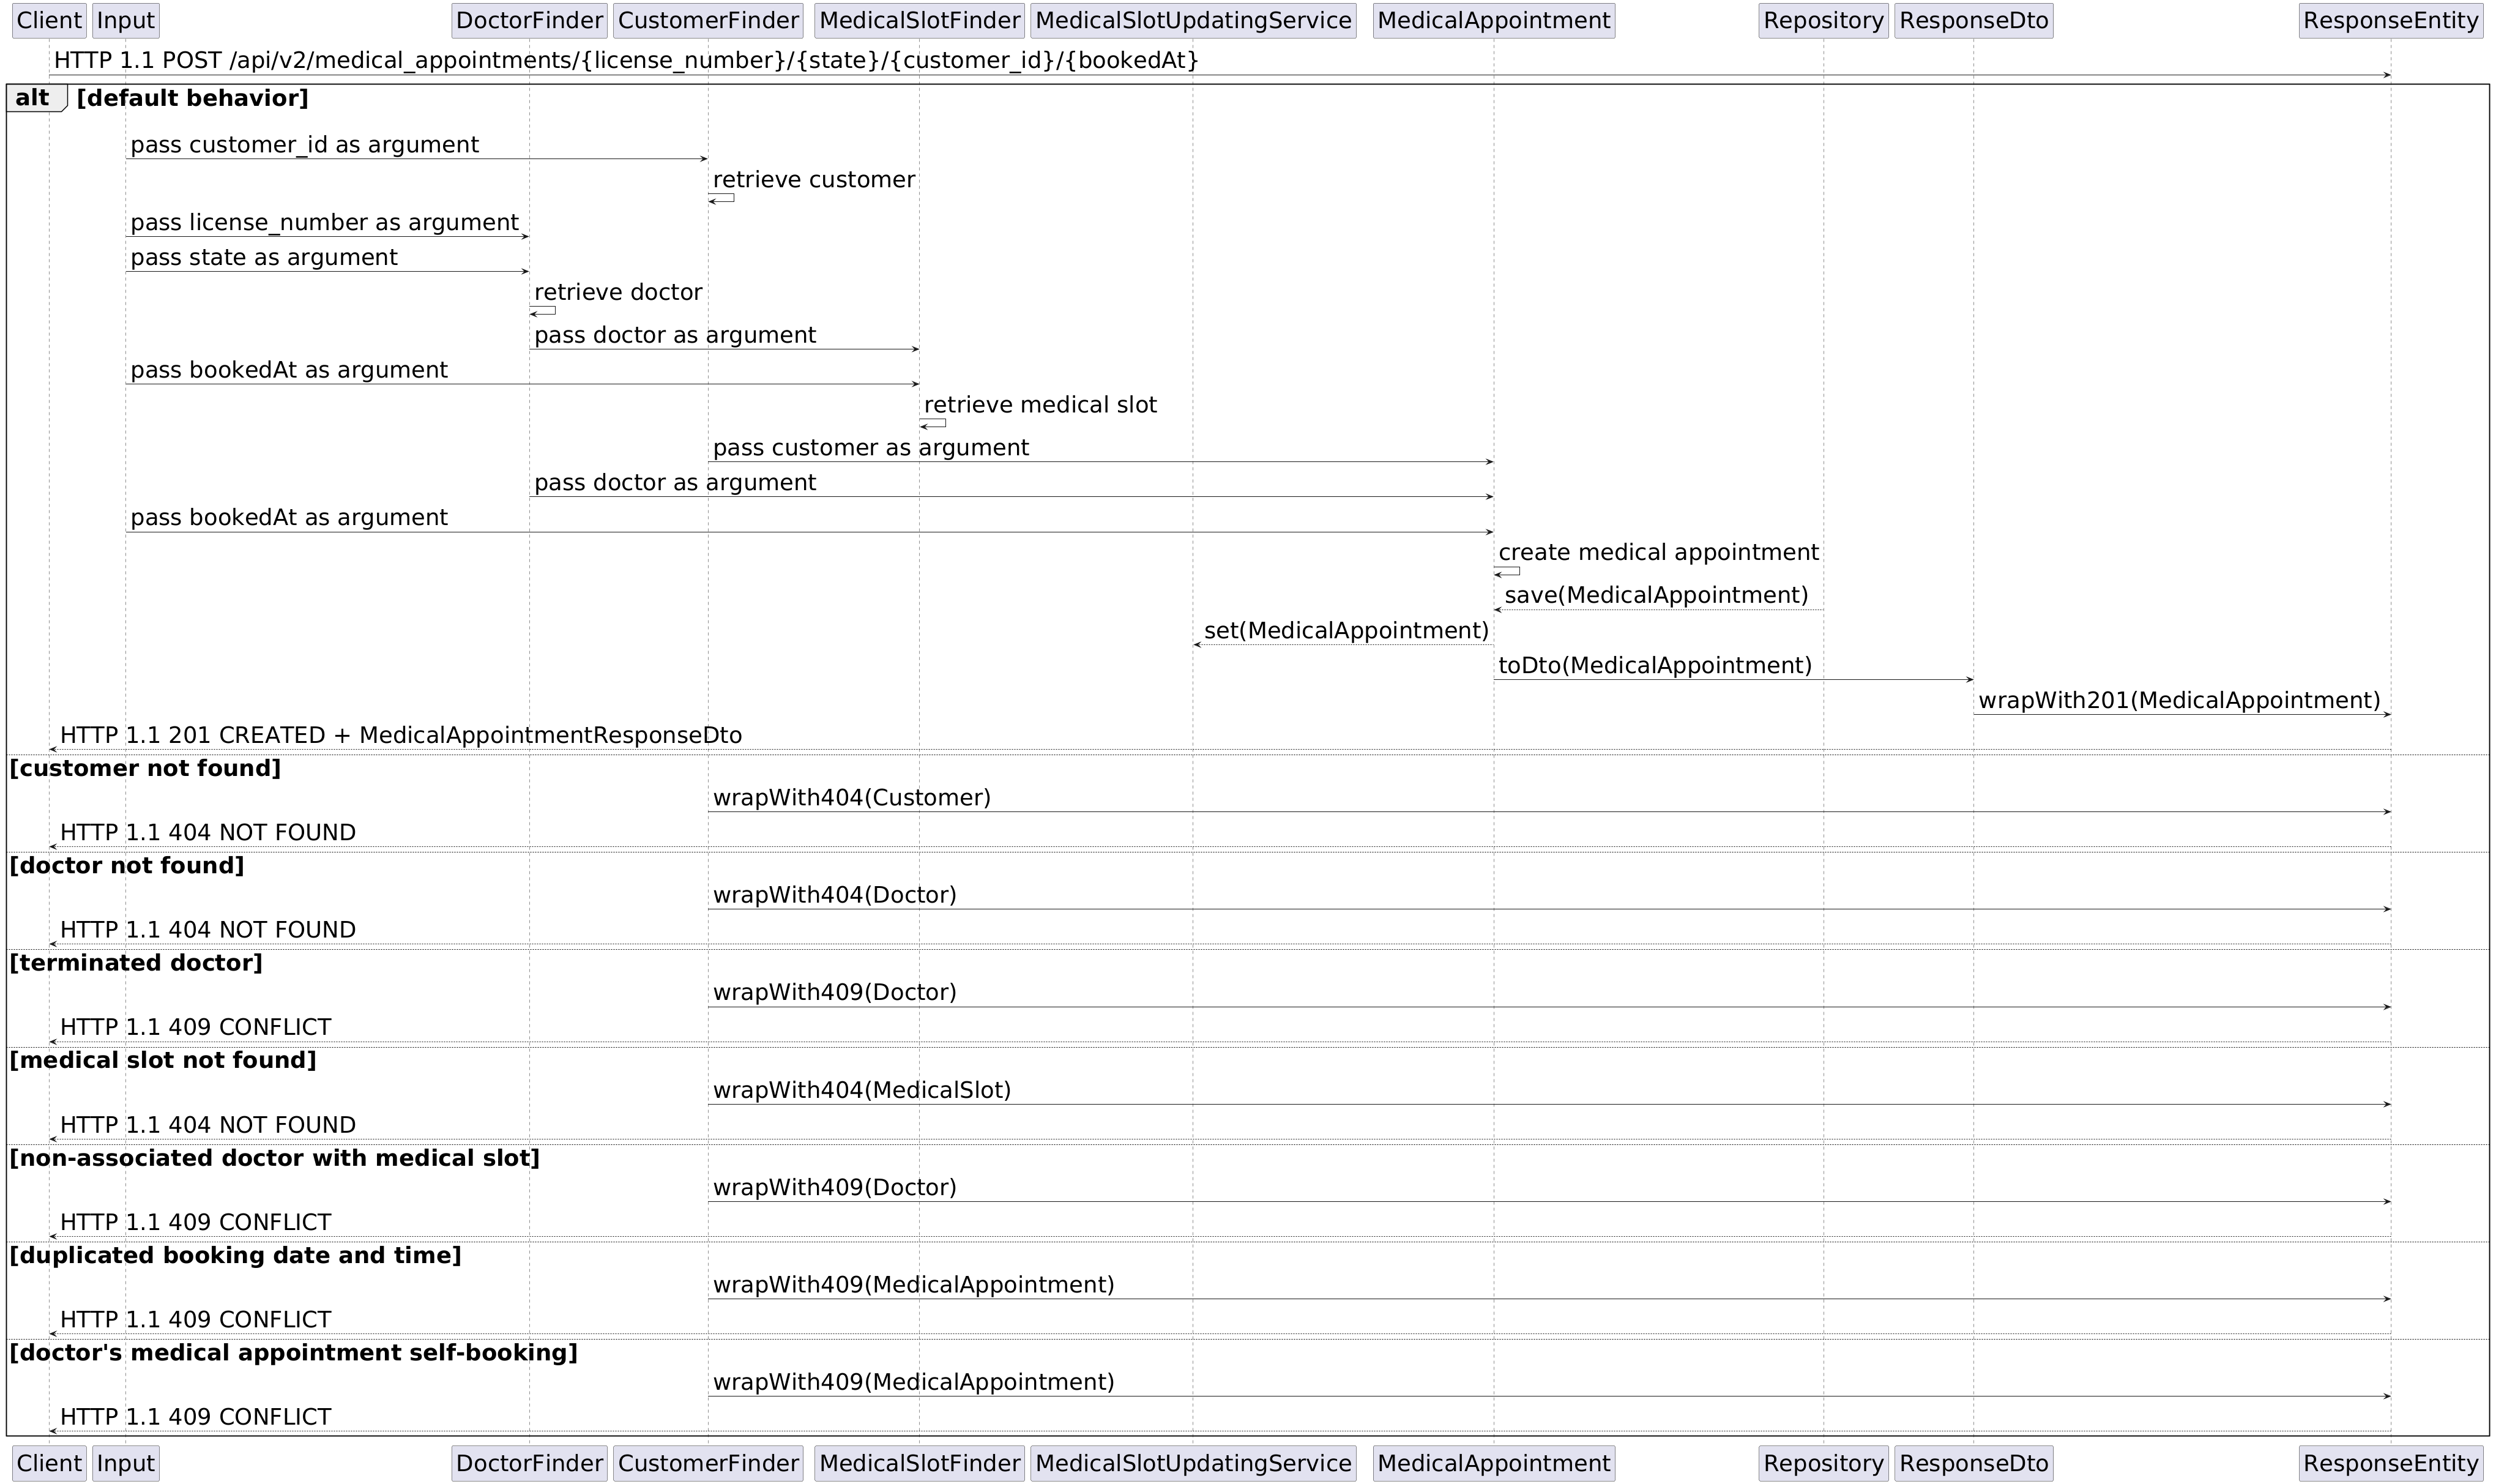
\includegraphics[width=0.99\linewidth]{figures/medical_appointment_registration_sequence_diagram}
		\\ \footnotesize Source: Author's creation.
		\label{fig:medical_appointment_registration_sequence_diagram}
	\end{figure}
\end{landscape}

The client, whose behavior is described in the \hyperref[subsection:http_semantics]{subsection HTTP Semantics}, requests a resource. It uses the \hyperref[appendix:glossary]{URI} \textit{/api/v2/medical\_appointments/\underline{license\_number}/\underline{state}/\underline{customer\_id}/\underline{booked\_at}}. The \hyperref[appendix:glossary]{URI} follows the pattern established  in the table \ref{tab:http-server-schemes}.

The path variables \textit{customer\_id}, \textit{license\_number}, \textit{state}, and \textit{booked\_at} are passed, respectively, to the \hyperref[appendix:glossary]{URI} \textit{/api/v2/medical\_appointments/\underline{license\_number}/\underline{state}/\underline{customer\_id}/\underline{booked\_at}} as arguments. The service creates a new \textbf{MedicalAppointment}, then persists it.

As exposed by the figure \ref{fig:medical_appointment_registration_sequence_diagram}, the default behavior is: firstly, \textbf{Customer} must be found. Then, \textbf{Doctor} is found. To retrieve both \textbf{Customer} and \textbf{Doctor}, the utility classes \textit{CustomerFinder} and \textit{DoctorFinder}, respectively. In order to retrieve the associated \textbf{MedicalSlot} with Doctor and \textit{booked\_at} as arguments of the utility class \textit{MedicalSlotFinder}, it retrieved to be changed in a near future step.

Considering the previous paragraph, a new instance of \textbf{MedicalAppointment} is created and persisted. Before it be turned into a \hyperref[appendix:glossary]{DTO}, the recently created \textbf{MedicalAppointment} fills the field \textit{medicalAppointment} of \textbf{MedicalSlot} via the service \textit{MedicalSlotUpdatingService}. 
After the mapping from the state of a persisted object to \hyperref[appendix:glossary]{DTO}, it is wrapped in the \hyperref[appendix:http_status_codes_summary_appendix]{status code 201}.

However, when either of the \textbf{Customer}, \textbf{Doctor} and \textbf{MedicalSlot} is null, the \hyperref[appendix:http_status_codes_summary_appendix]{status code 404} is returned. Nonetheless, when either of the duplicated booking date and time is provided, the sought \textbf{Doctor} is terminated, the sought \textbf{Doctor} seeks to booking a medical appointment whose associated medical slot's doctor is them, the  \hyperref[appendix:http_status_codes_summary_appendix]{status code 409} is returned.

\subsubsection{Successful Case}

\begin{figure}[H]
	\centering
	\caption{Medical Appointment Registration Successful Case}
	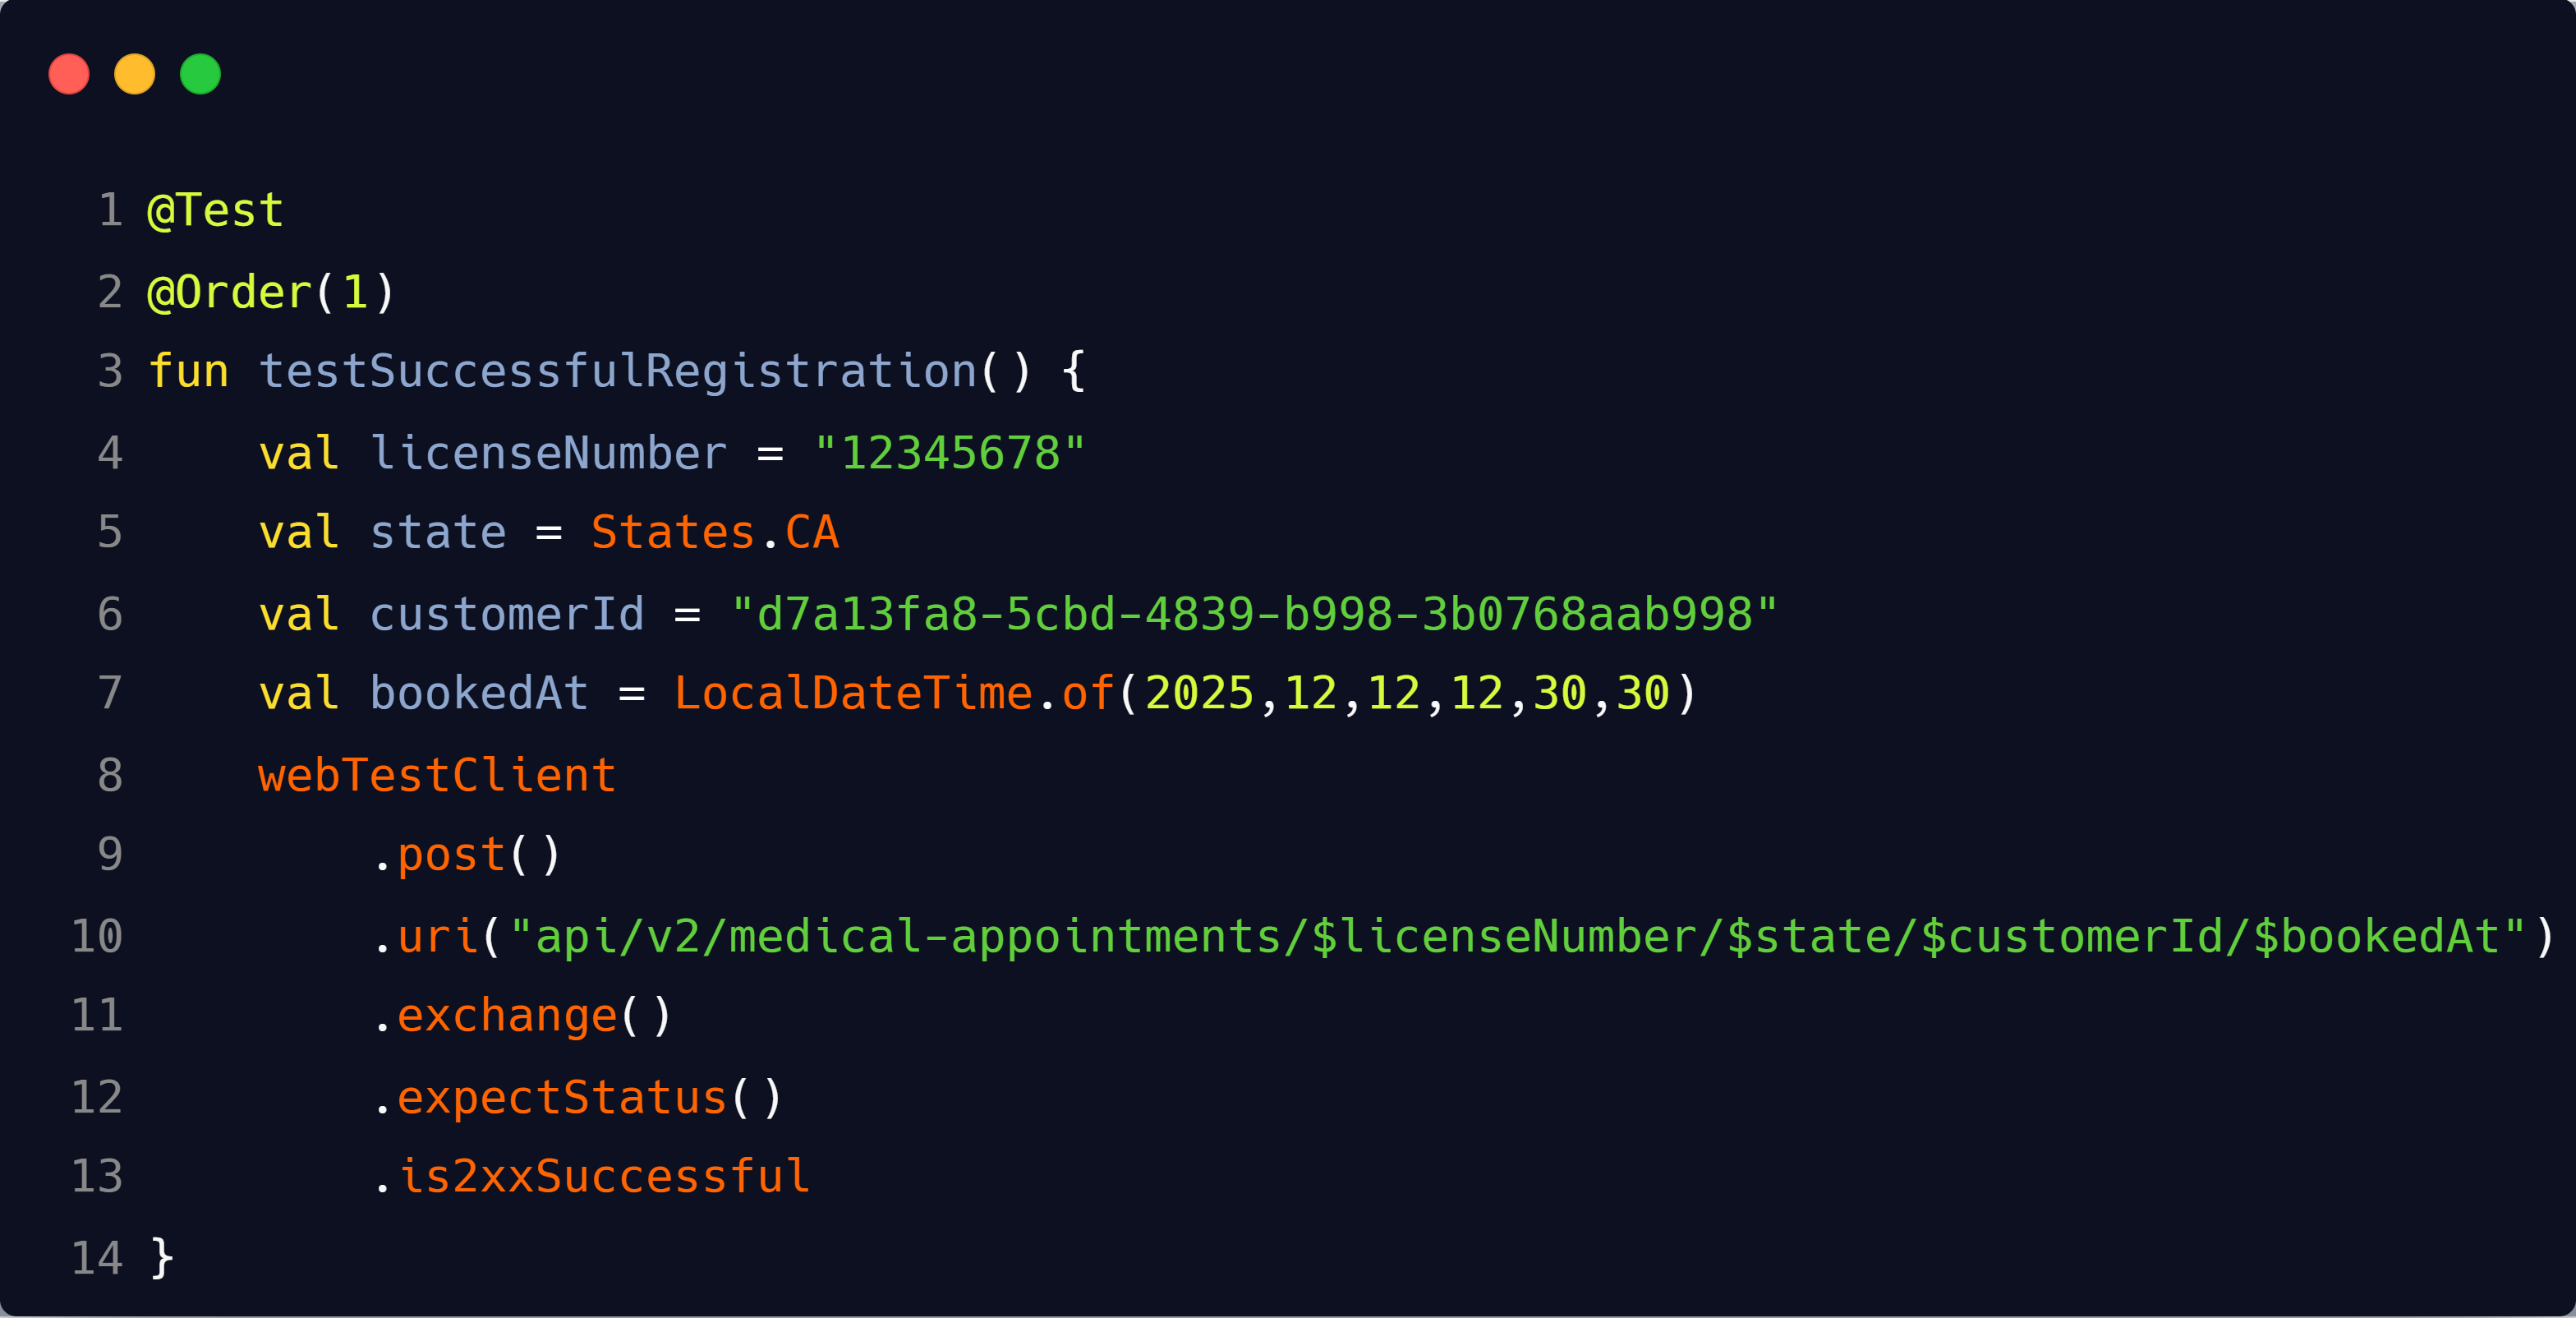
\includegraphics[width=1\linewidth]{figures/medical_appointment_registration_integration_test_successful_case.png}
	\label{fig:medical_appointment_registration_integration_test_successful_case}
	\footnotesize Source: Author's creation.
\end{figure}

The method \textit{testSuccessfulRegistration} uses an instance of the \textit{WebTestClient}, as argued by the \hyperref[subsection:automated_software_testing]{subsection Automated Software Testing}. In order to register a \textbf{MedicalAppointment}, the POST method was used. As clarified by the \hyperref[subsection:http_semantics]{subsection HTTP Semantics}, every HTTP request requires a \hyperref[appendix:glossary]{URI} to route the expected request to the target server aiming to obtain the expected result. Thereby, the \hyperref[appendix:glossary]{URI} \textit{/api/v2/medical\_appointments/\underline{license\_number}/\underline{state}/\underline{customer\_id}/\underline{available\_at}} is placed as the argument of \textit{uri()}. Finally, the \hyperref[tab:summary_http_status_codes]{status code 201} is returned.

\subsubsection{Unsuccessful Case: Customer Not Found}

\begin{figure}[H]
	\centering
	\caption{Medical Appointment Registration Unsuccessful Case: Customer Not Found}
	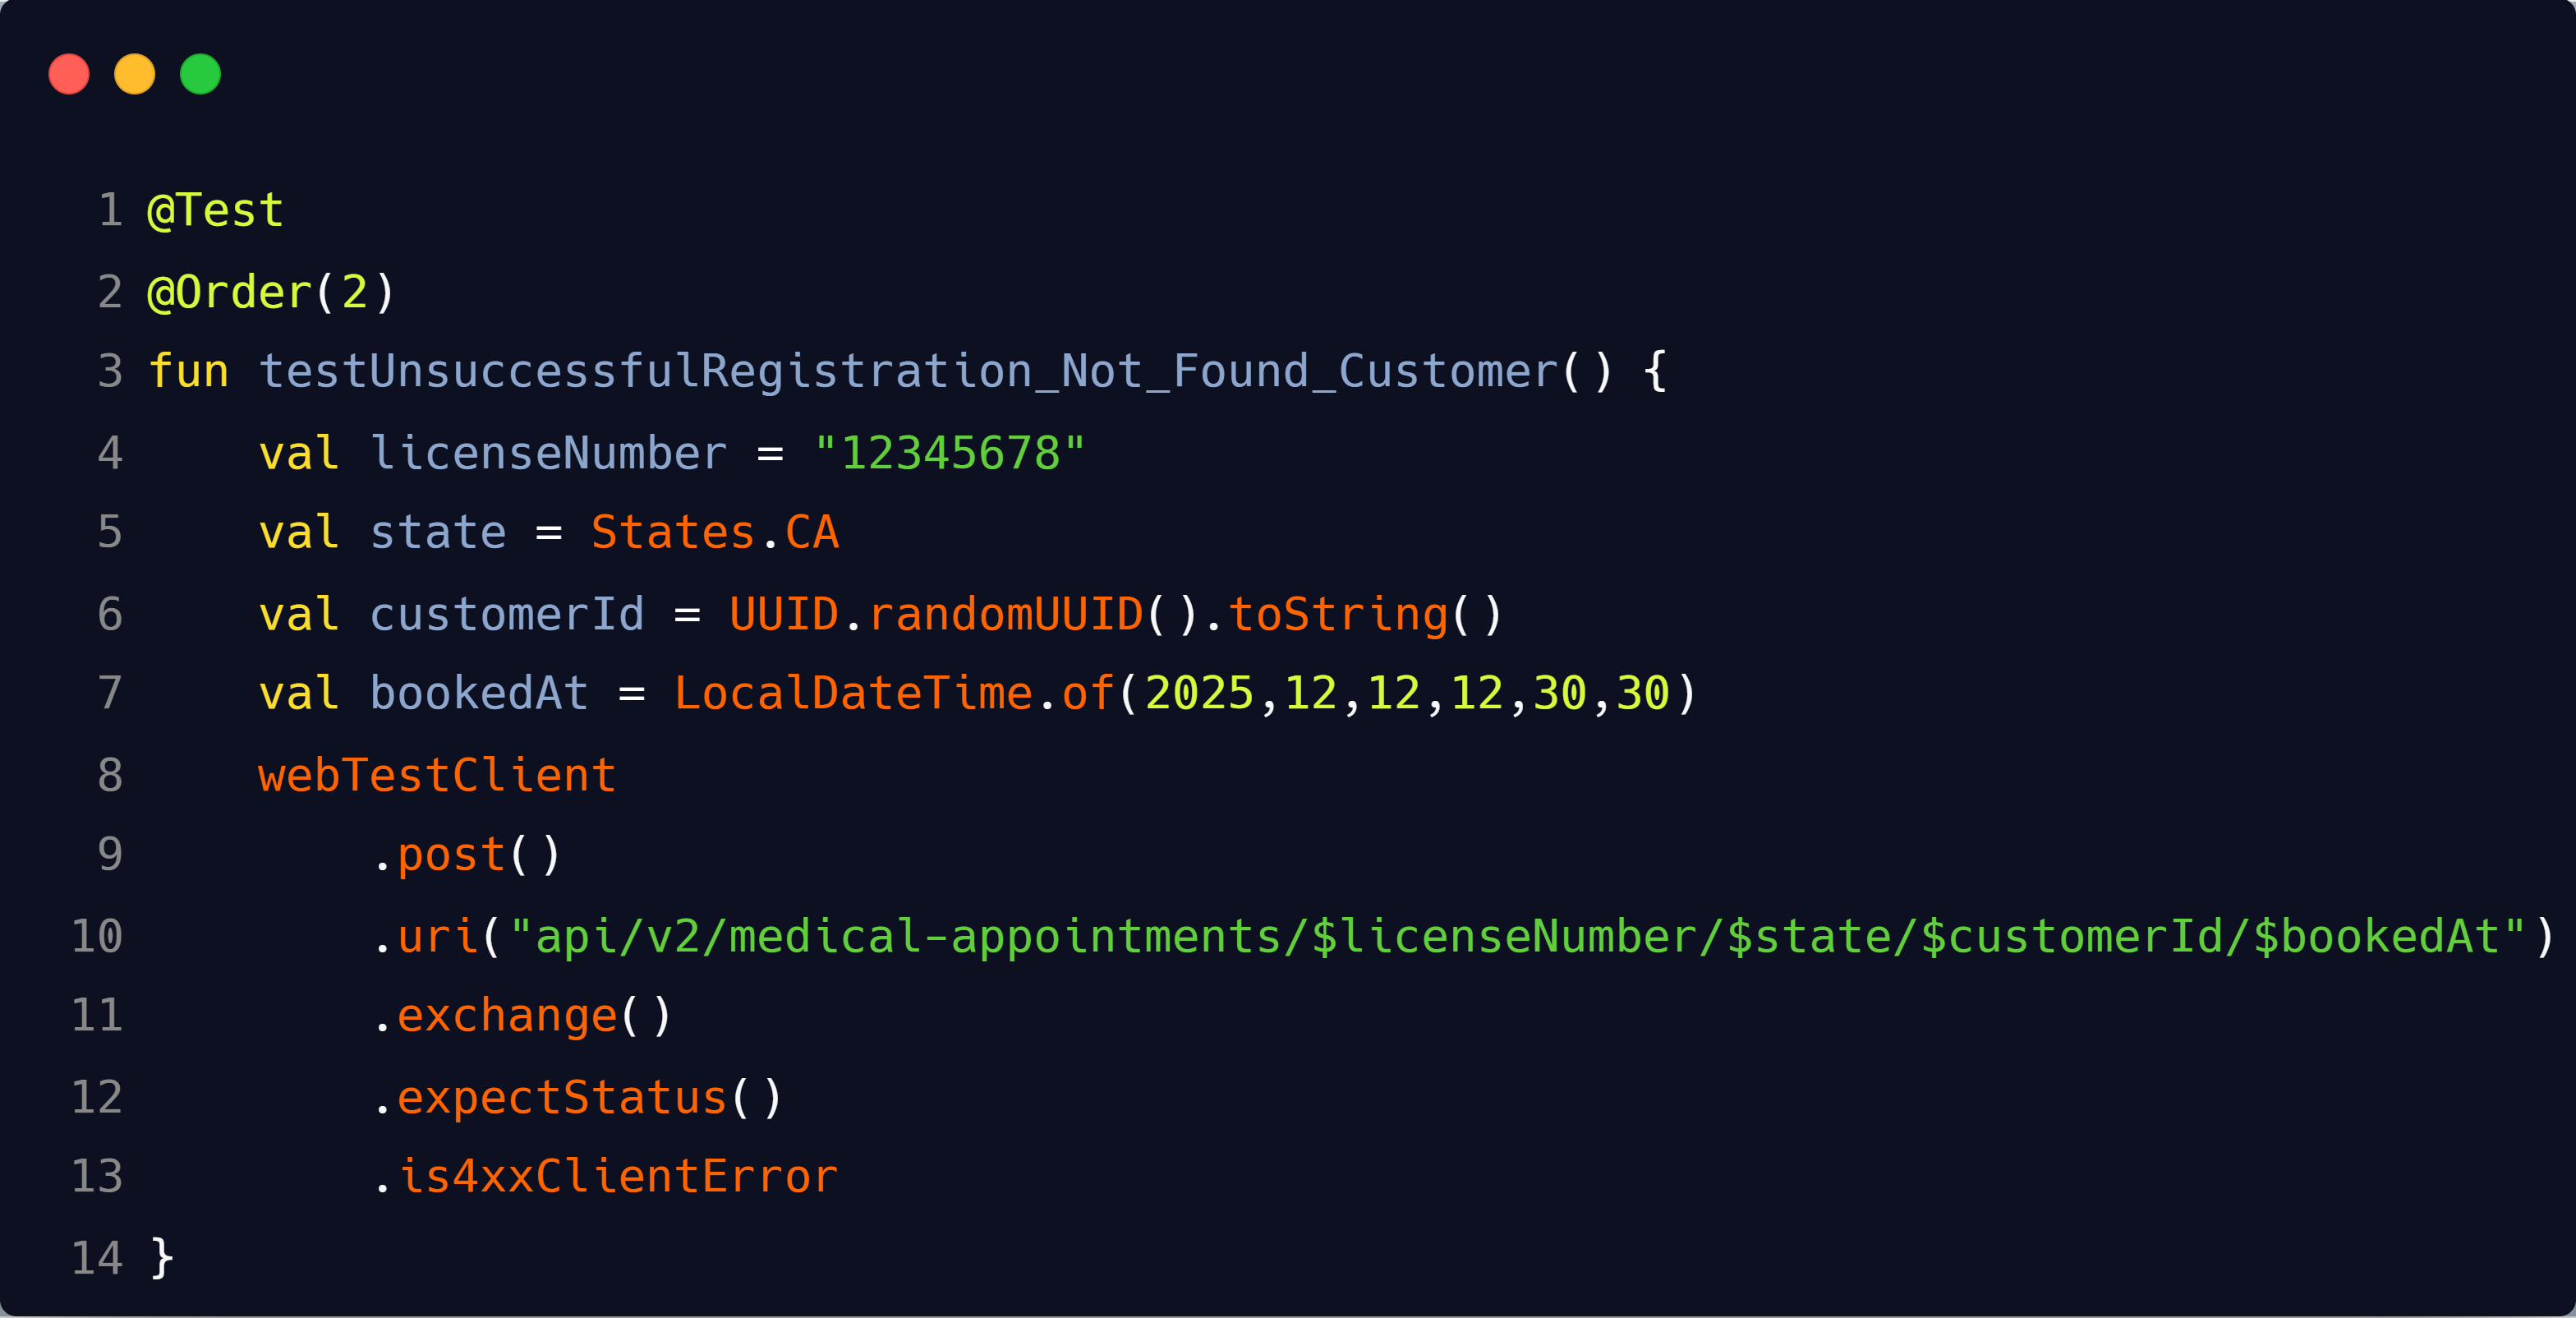
\includegraphics[width=1\linewidth]{figures/medical_appointment_registration_integration_test_unsuccessful_case_customer_not_found.png}
	\label{fig:medical_appointment_registration_integration_test_unsuccessful_case_customer_not_found}
	\footnotesize Source: Author's creation.
\end{figure}

The method \textit{testUnsuccessfulRegistration\_Doctor\_Self\_Booking} uses an instance of the \textit{WebTestClient}, as argued by the \hyperref[subsection:automated_software_testing]{subsection Automated Software Testing}. When, at the moment that validated input data is extracted from the path variables \textit{customer\_id}, \textit{license\_number}, \textit{state}, and \textit{booked\_at}, and it is discovered that the sought \textbf{Customer} is null, the \hyperref[tab:summary_http_status_codes]{status code 404} is returned.

\subsubsection{Unsuccessful Case: Doctor Not Found}

\begin{figure}[H]
	\centering
	\caption{Medical Appointment Registration Unsuccessful Case: Terminated Doctor}
	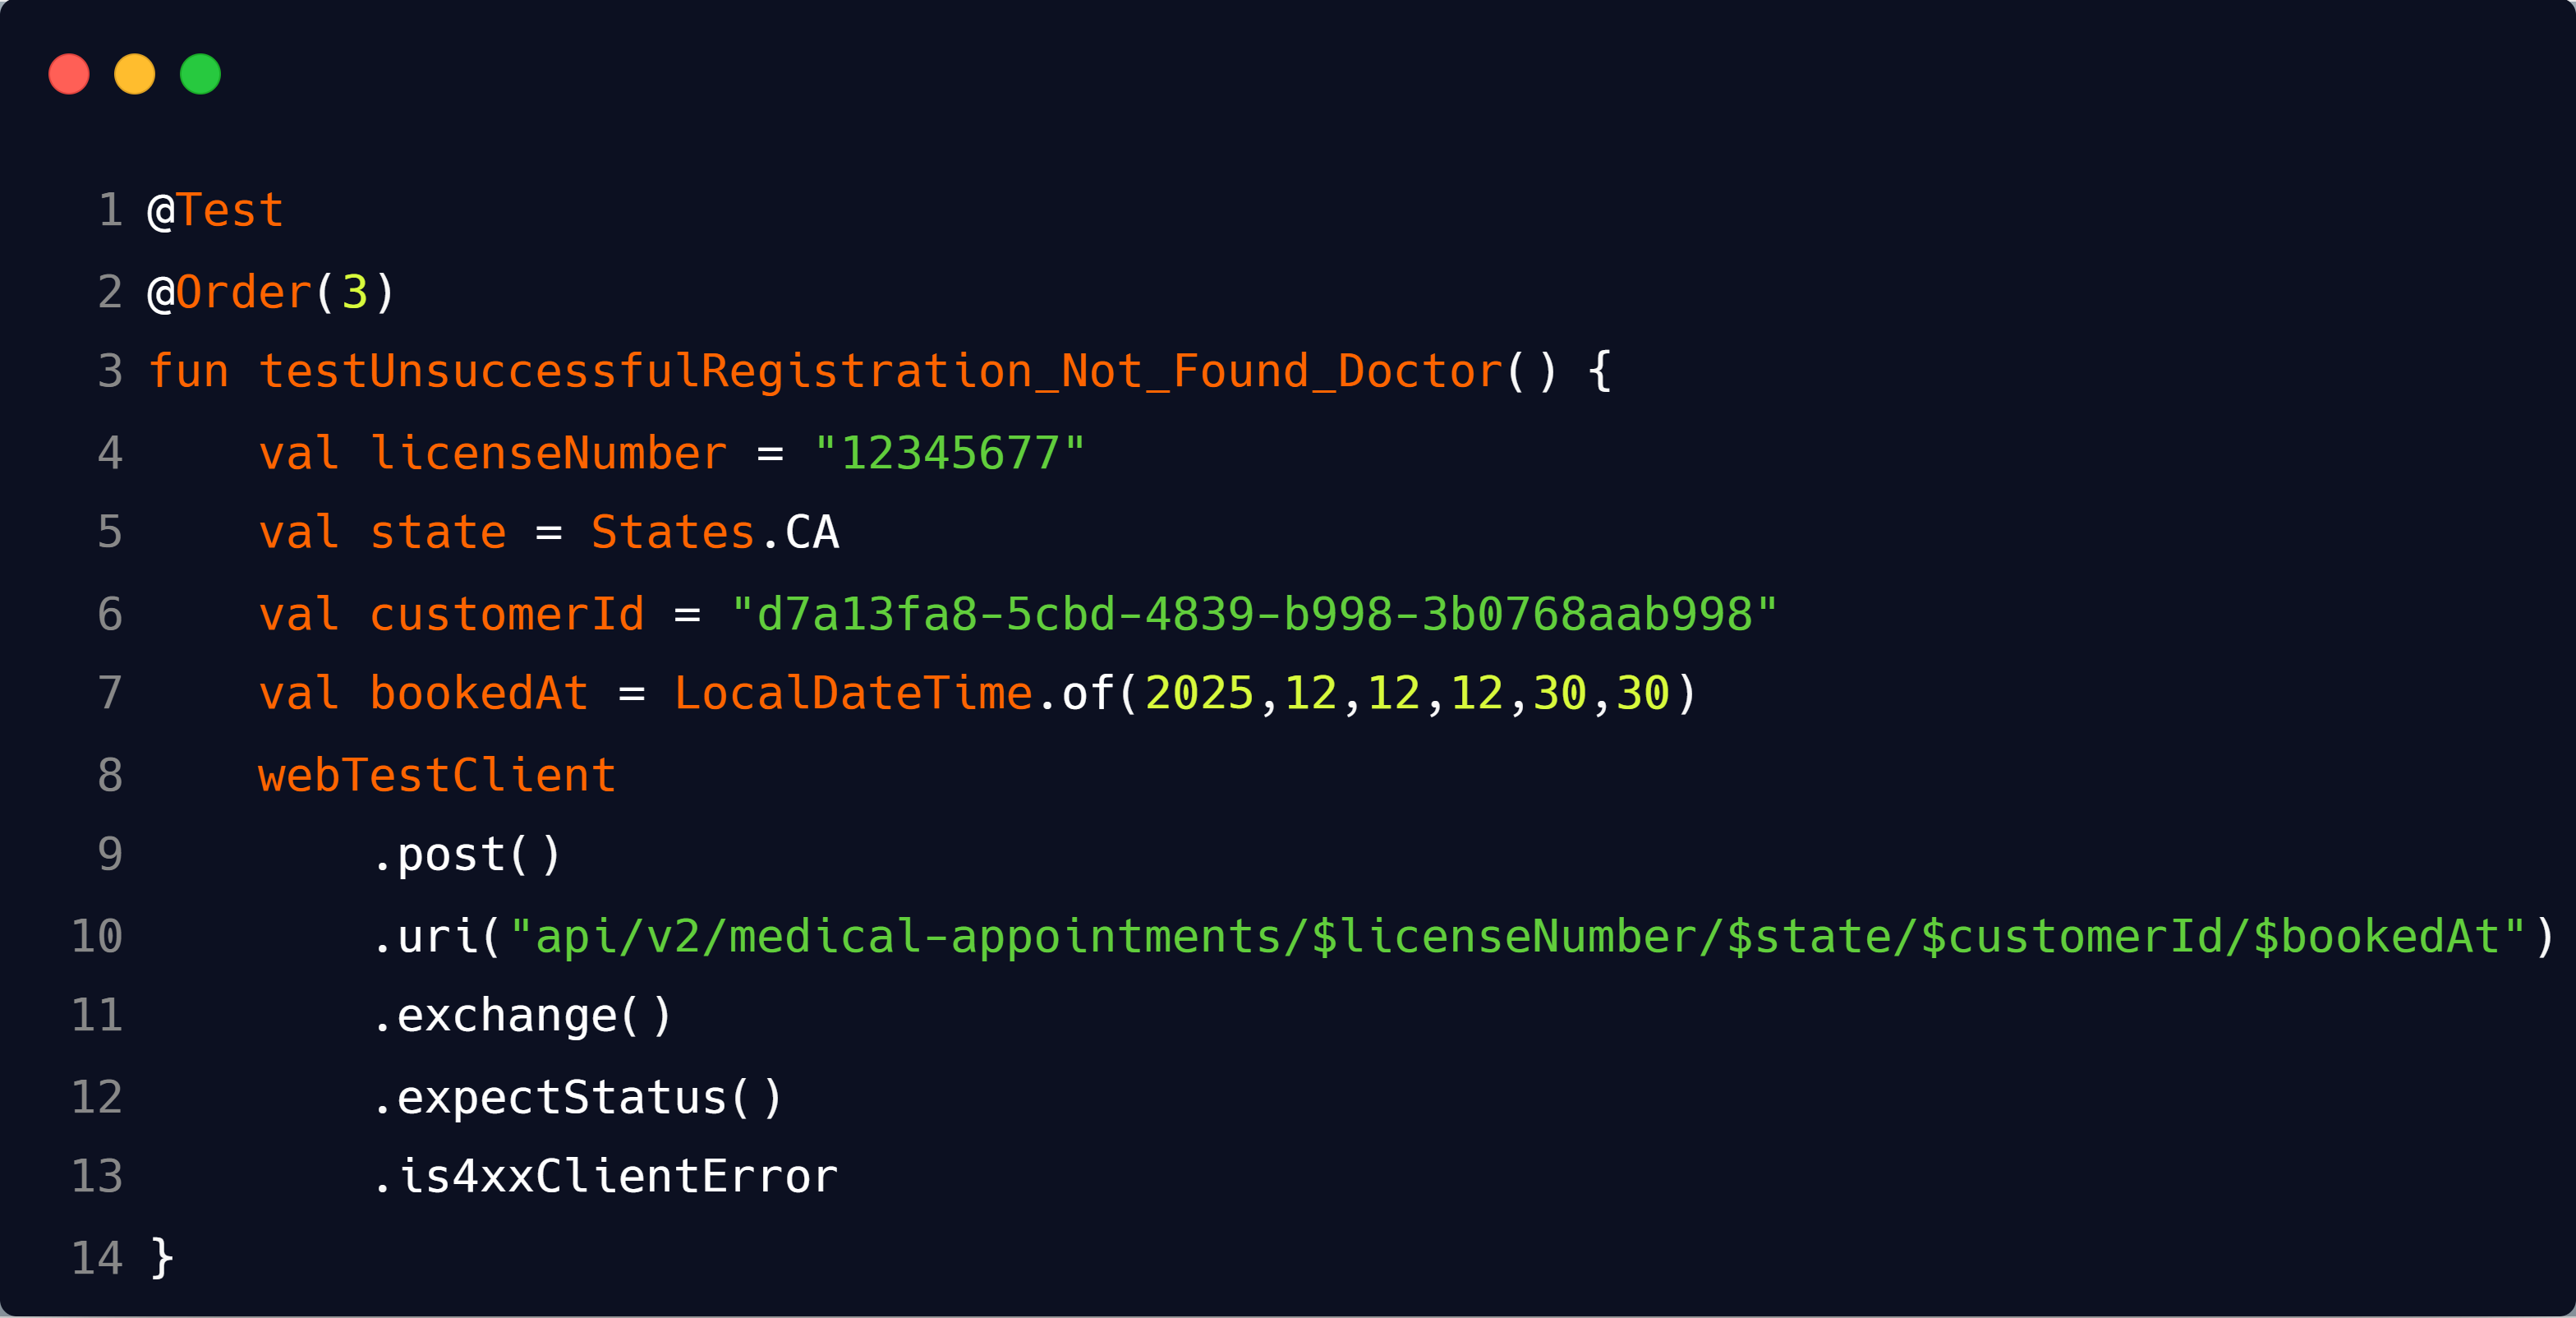
\includegraphics[width=1\linewidth]{figures/medical_appointment_registration_integration_test_unsuccessful_case_doctor_not_found.png}
	\label{fig:/medical_appointment_registration_integration_test_unsuccessful_case_doctor_not_found}
	\footnotesize Source: Author's creation.
\end{figure}

The method \textit{testUnsuccessfulRegistration\_Doctor\_Self\_Booking} uses an instance of the \textit{WebTestClient}, as argued by the \hyperref[subsection:automated_software_testing]{subsection Automated Software Testing}. When, at the moment that validated input data is extracted from the path variables \textit{customer\_id}, \textit{license\_number}, \textit{state}, and \textit{booked\_at}, and it is discovered that the sought \textbf{Doctor} is null, the \hyperref[tab:summary_http_status_codes]{status code 404} is returned.

\subsubsection{Unsuccessful Case: Terminated Doctor}

\begin{figure}[H]
	\centering
	\caption{Medical Appointment Registration Unsuccessful Case: Terminated Doctor}
	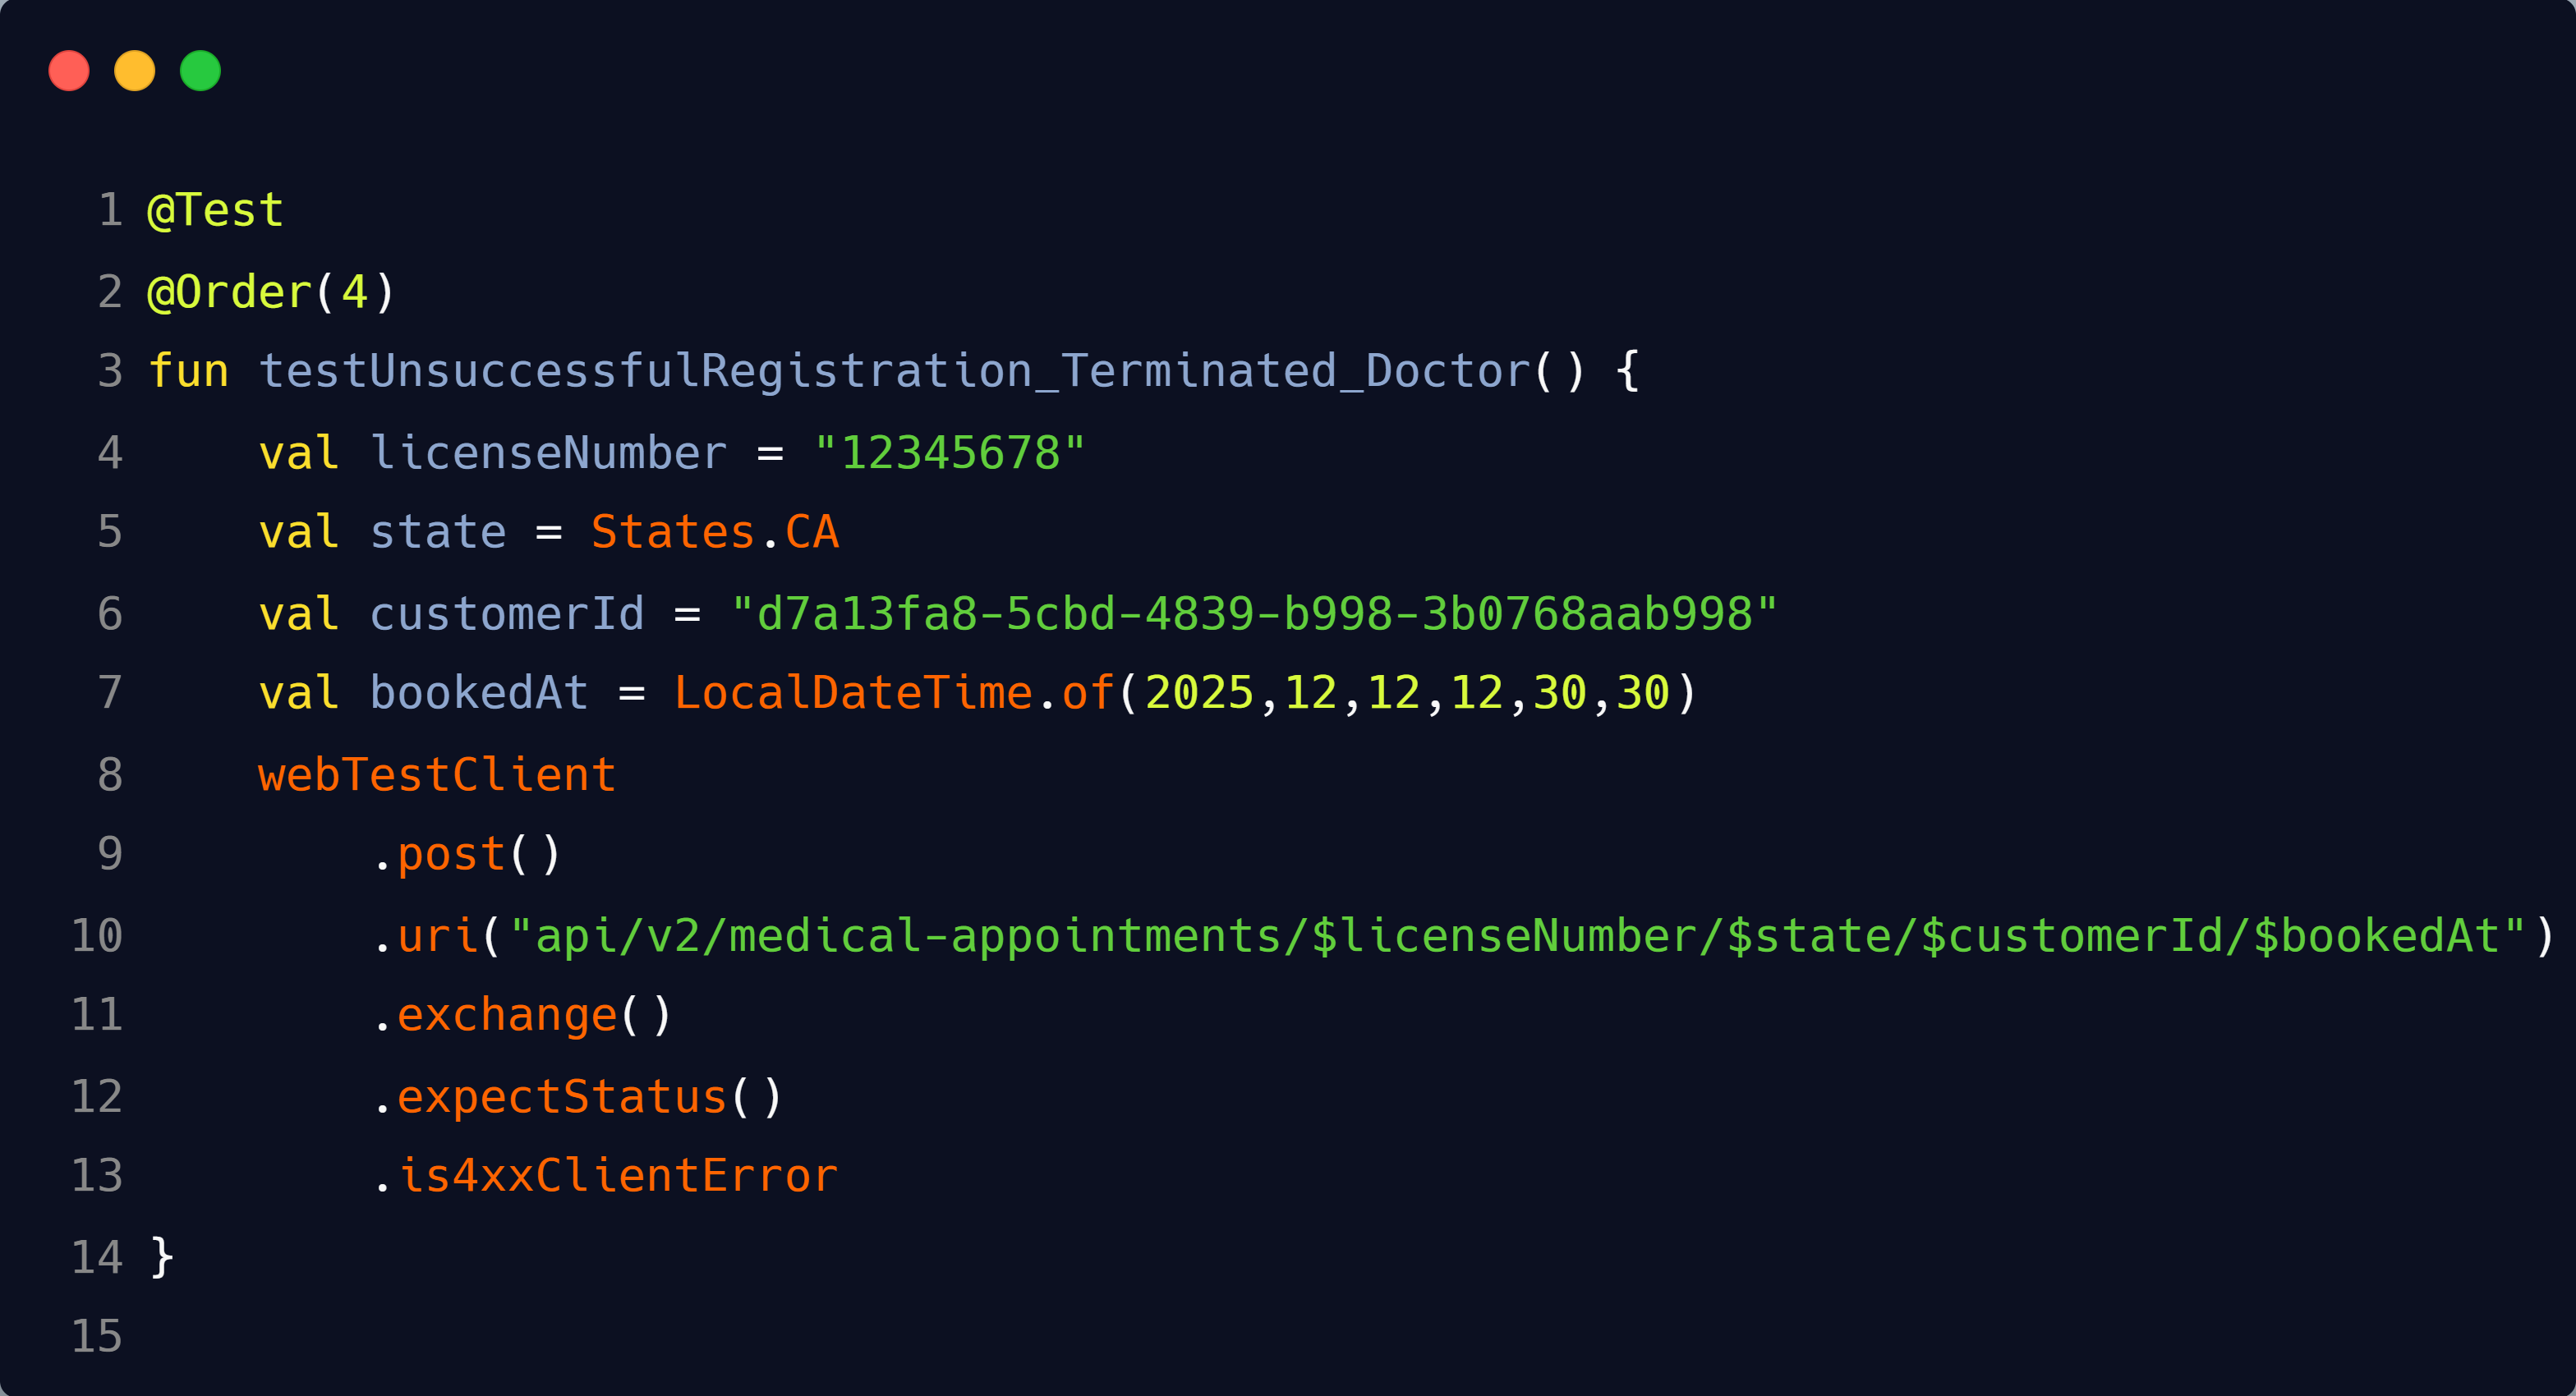
\includegraphics[width=1\linewidth]{figures/medical_appointment_registration_integration_test_unsuccessful_case_terminated_doctor.png}
	\label{fig:medical_appointment_registration_integration_test_unsuccessful_case_terminated_doctor}
	\footnotesize Source: Author's creation.
\end{figure}

The method \textit{testUnsuccessfulRegistration\_Doctor\_Self\_Booking} uses an instance of the \textit{WebTestClient}, as argued by the \hyperref[subsection:automated_software_testing]{subsection Automated Software Testing}. When, at the moment that validated input data is extracted from the path variables \textit{customer\_id}, \textit{license\_number}, \textit{state}, and \textit{booked\_at}, and it is discovered that the sought \textbf{Doctor} is terminated, the \hyperref[tab:summary_http_status_codes]{status code 409} is returned.

\subsubsection{Unsuccessful Case: Medical Slot Not Found}

\begin{figure}[H]
	\centering
	\caption{Medical Appointment Registration Unsuccessful Case: Medical Slot Not Found}
	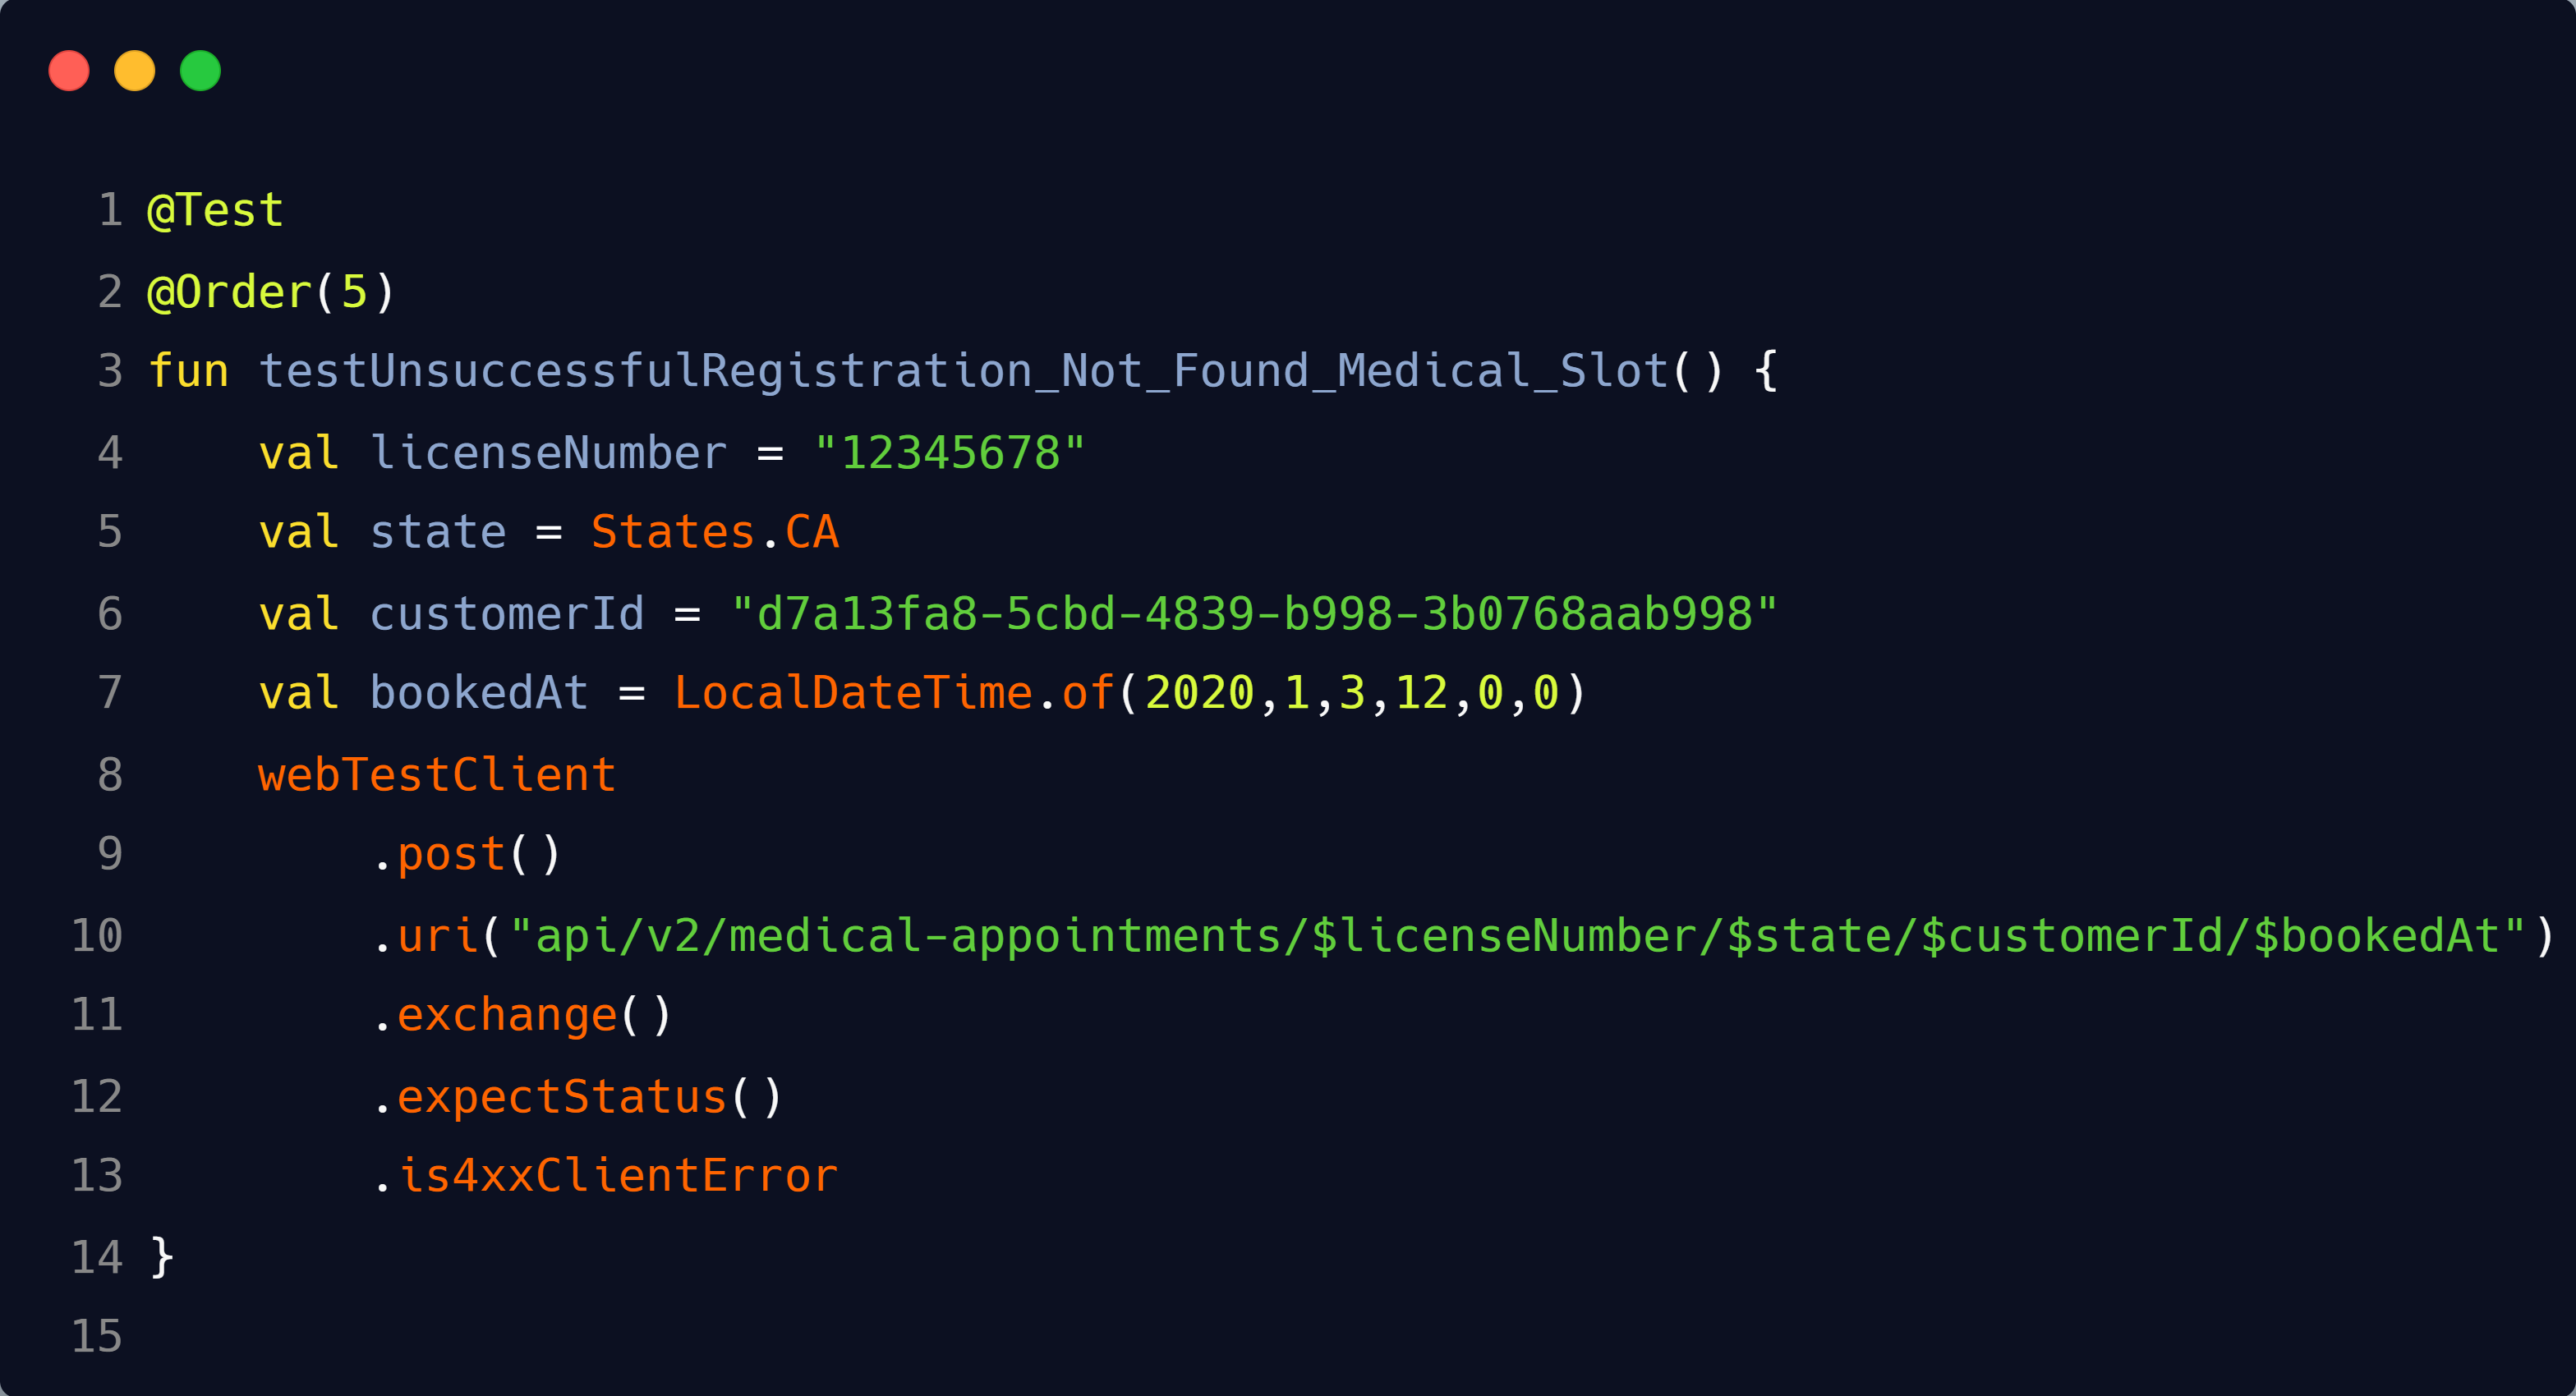
\includegraphics[width=1\linewidth]{figures/medical_appointment_registration_integration_test_unsuccessful_case_medical_slot_not_found.png}
	\label{fig:/medical_appointment_registration_integration_test_unsuccessful_case_medical_slot_not_found}
	\footnotesize Source: Author's creation.
\end{figure}

The method \textit{testUnsuccessfulRegistration\_Doctor\_Self\_Booking} uses an instance of the \textit{WebTestClient}, as argued by the \hyperref[subsection:automated_software_testing]{subsection Automated Software Testing}. When, at the moment that validated input data is extracted from the path variables \textit{customer\_id}, \textit{license\_number}, \textit{state}, and \textit{booked\_at}, and it is discovered that the sought \textbf{MedicalSlot} is null, the \hyperref[tab:summary_http_status_codes]{status code 404} is returned.

\subsubsection{Unsuccessful Case: Non-Associated Doctor With Medical Slot}

\begin{figure}[H]
	\centering
	\caption{Medical Appointment Registration Unsuccessful Case: Non-Associated Doctor With Medical Slot}
	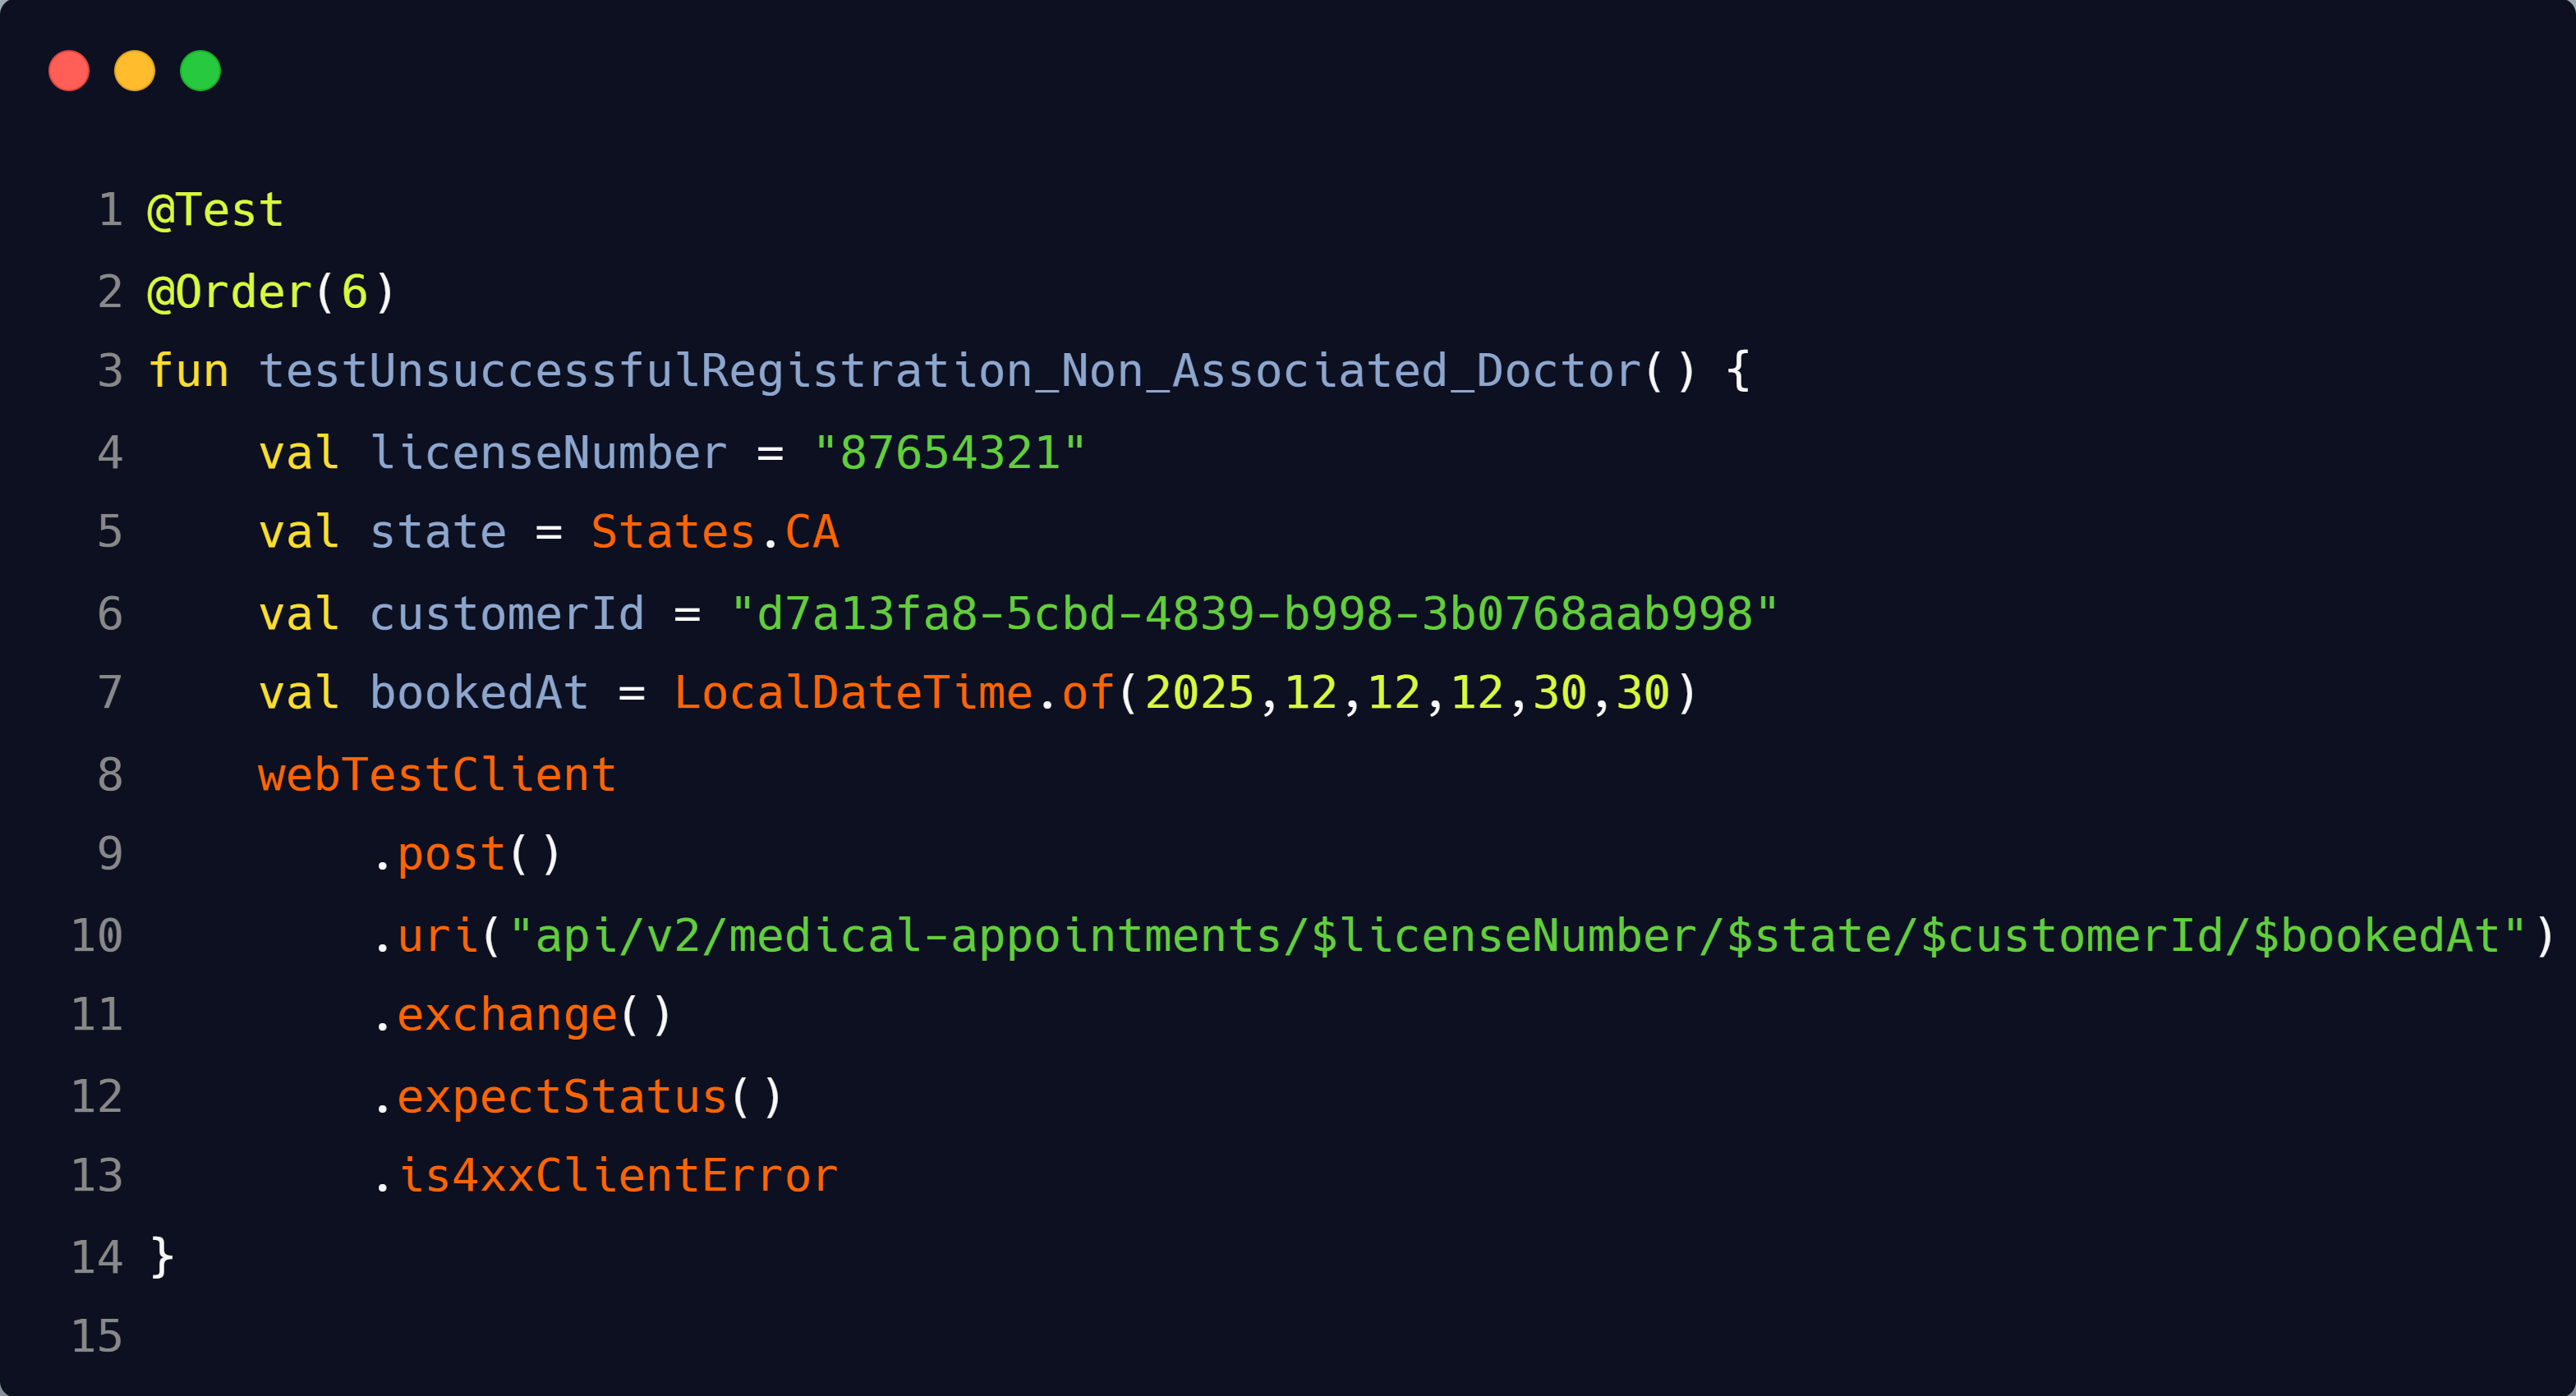
\includegraphics[width=1\linewidth]{figures/medical_appointment_registration_integration_test_unsuccessful_case_nonassociated_doctor.png}
	\label{fig:medical_appointment_registration_integration_test_unsuccessful_case_nonassociated_doctor}
	\footnotesize Source: Author's creation.
\end{figure}

The method \textit{testUnsuccessfulRegistration\_Doctor\_Self\_Booking} uses an instance of the \textit{WebTestClient}, as argued by the \hyperref[subsection:automated_software_testing]{subsection Automated Software Testing}. When, at the moment that validated input data is extracted from the path variables \textit{customer\_id}, \textit{license\_number}, \textit{state}, and \textit{booked\_at}, and it is discovered that the sought \textbf{Doctor} is not the sought \textbf{MedicalSlot}'s doctor, the \hyperref[tab:summary_http_status_codes]{status code 409} is returned.

\subsubsection{Unsuccessful Case: Duplicated Booking Date And Time}

\begin{figure}[H]
	\centering
	\caption{Medical Appointment Registration Unsuccessful Case: Duplicated Booking Date And Time}
	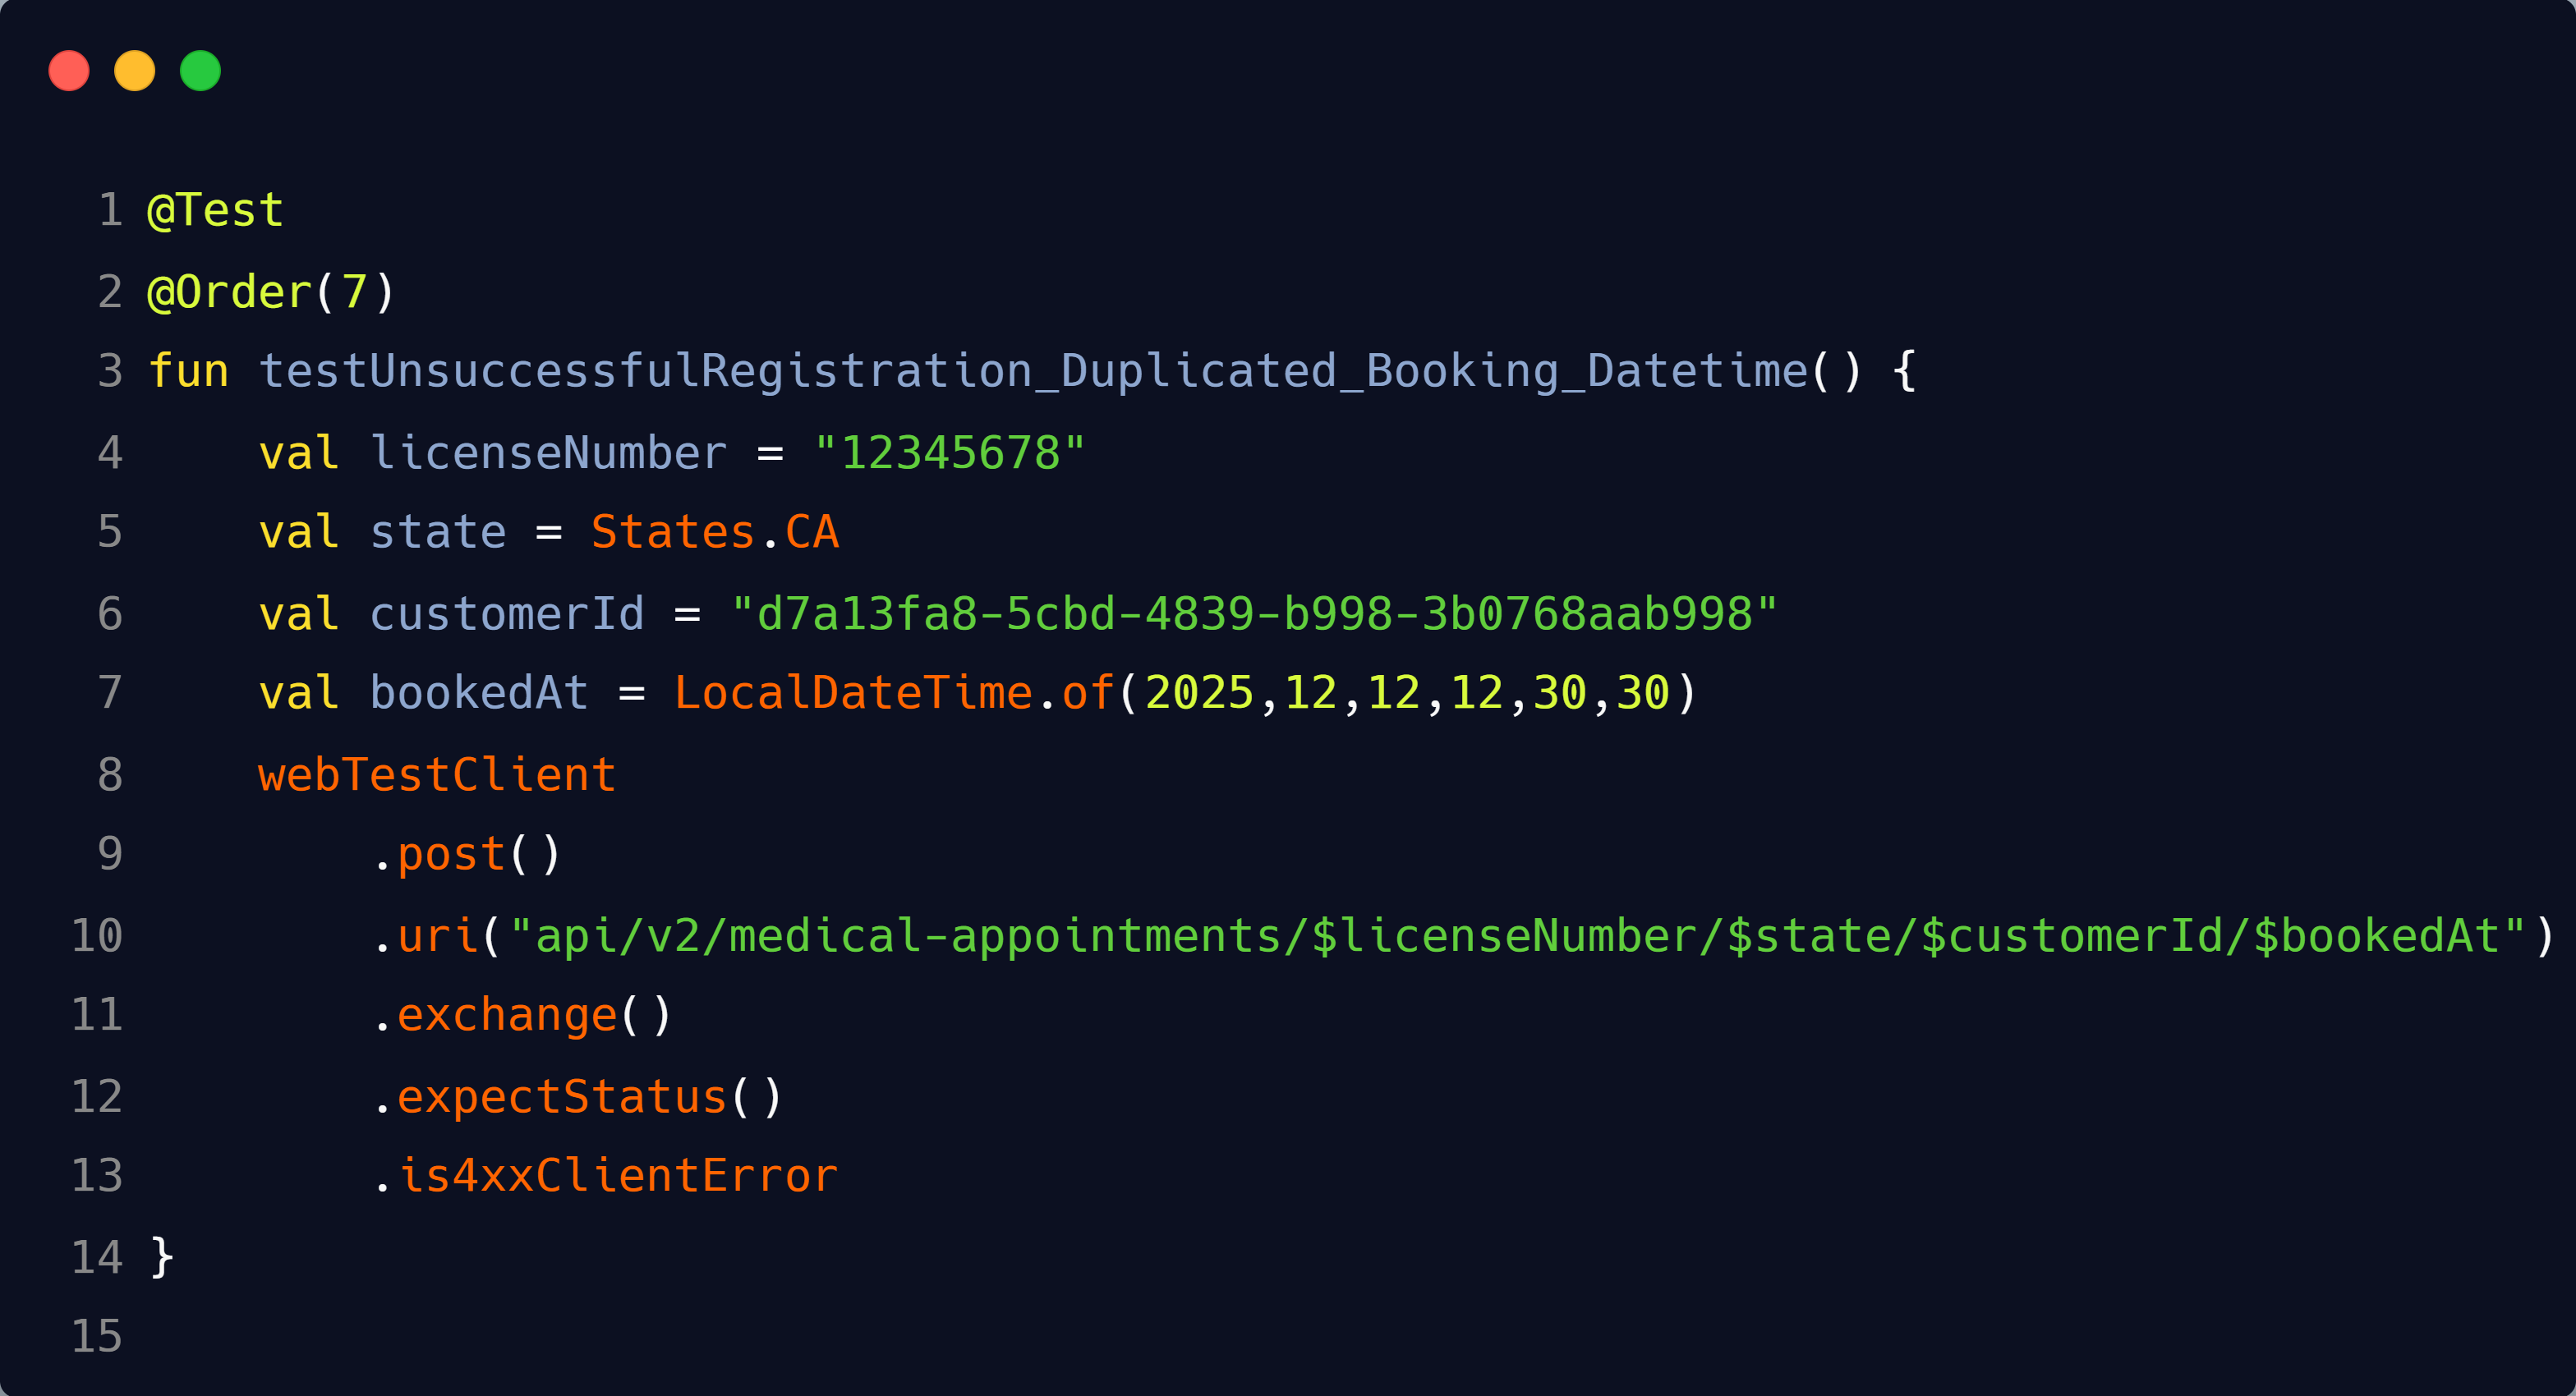
\includegraphics[width=1\linewidth]{figures/medical_appointment_registration_integration_test_unsuccessful_case_duplicared_booking_datetime.png}
	\label{fig:medical_appointment_registration_integration_test_unsuccessful_case_duplicared_booking_datetime}
	\footnotesize Source: Author's creation.
\end{figure}

The method \textit{testUnsuccessfulRegistration\_Doctor\_Self\_Booking} uses an instance of the \textit{WebTestClient}, as argued by the \hyperref[subsection:automated_software_testing]{subsection Automated Software Testing}. When, at the moment that validated input data is extracted from the path variables \textit{customer\_id}, \textit{license\_number}, \textit{state}, and \textit{booked\_at}, and it is discovered that provided booking date and time, the \hyperref[tab:summary_http_status_codes]{status code 409} is returned.

\subsubsection{Unsuccessful Case: Doctor's Medical Appointment Self-Booking}

\begin{figure}[H]
	\centering
	\caption{Medical Appointment Registration Unsuccessful Case: Doctor's Self-Booking}
	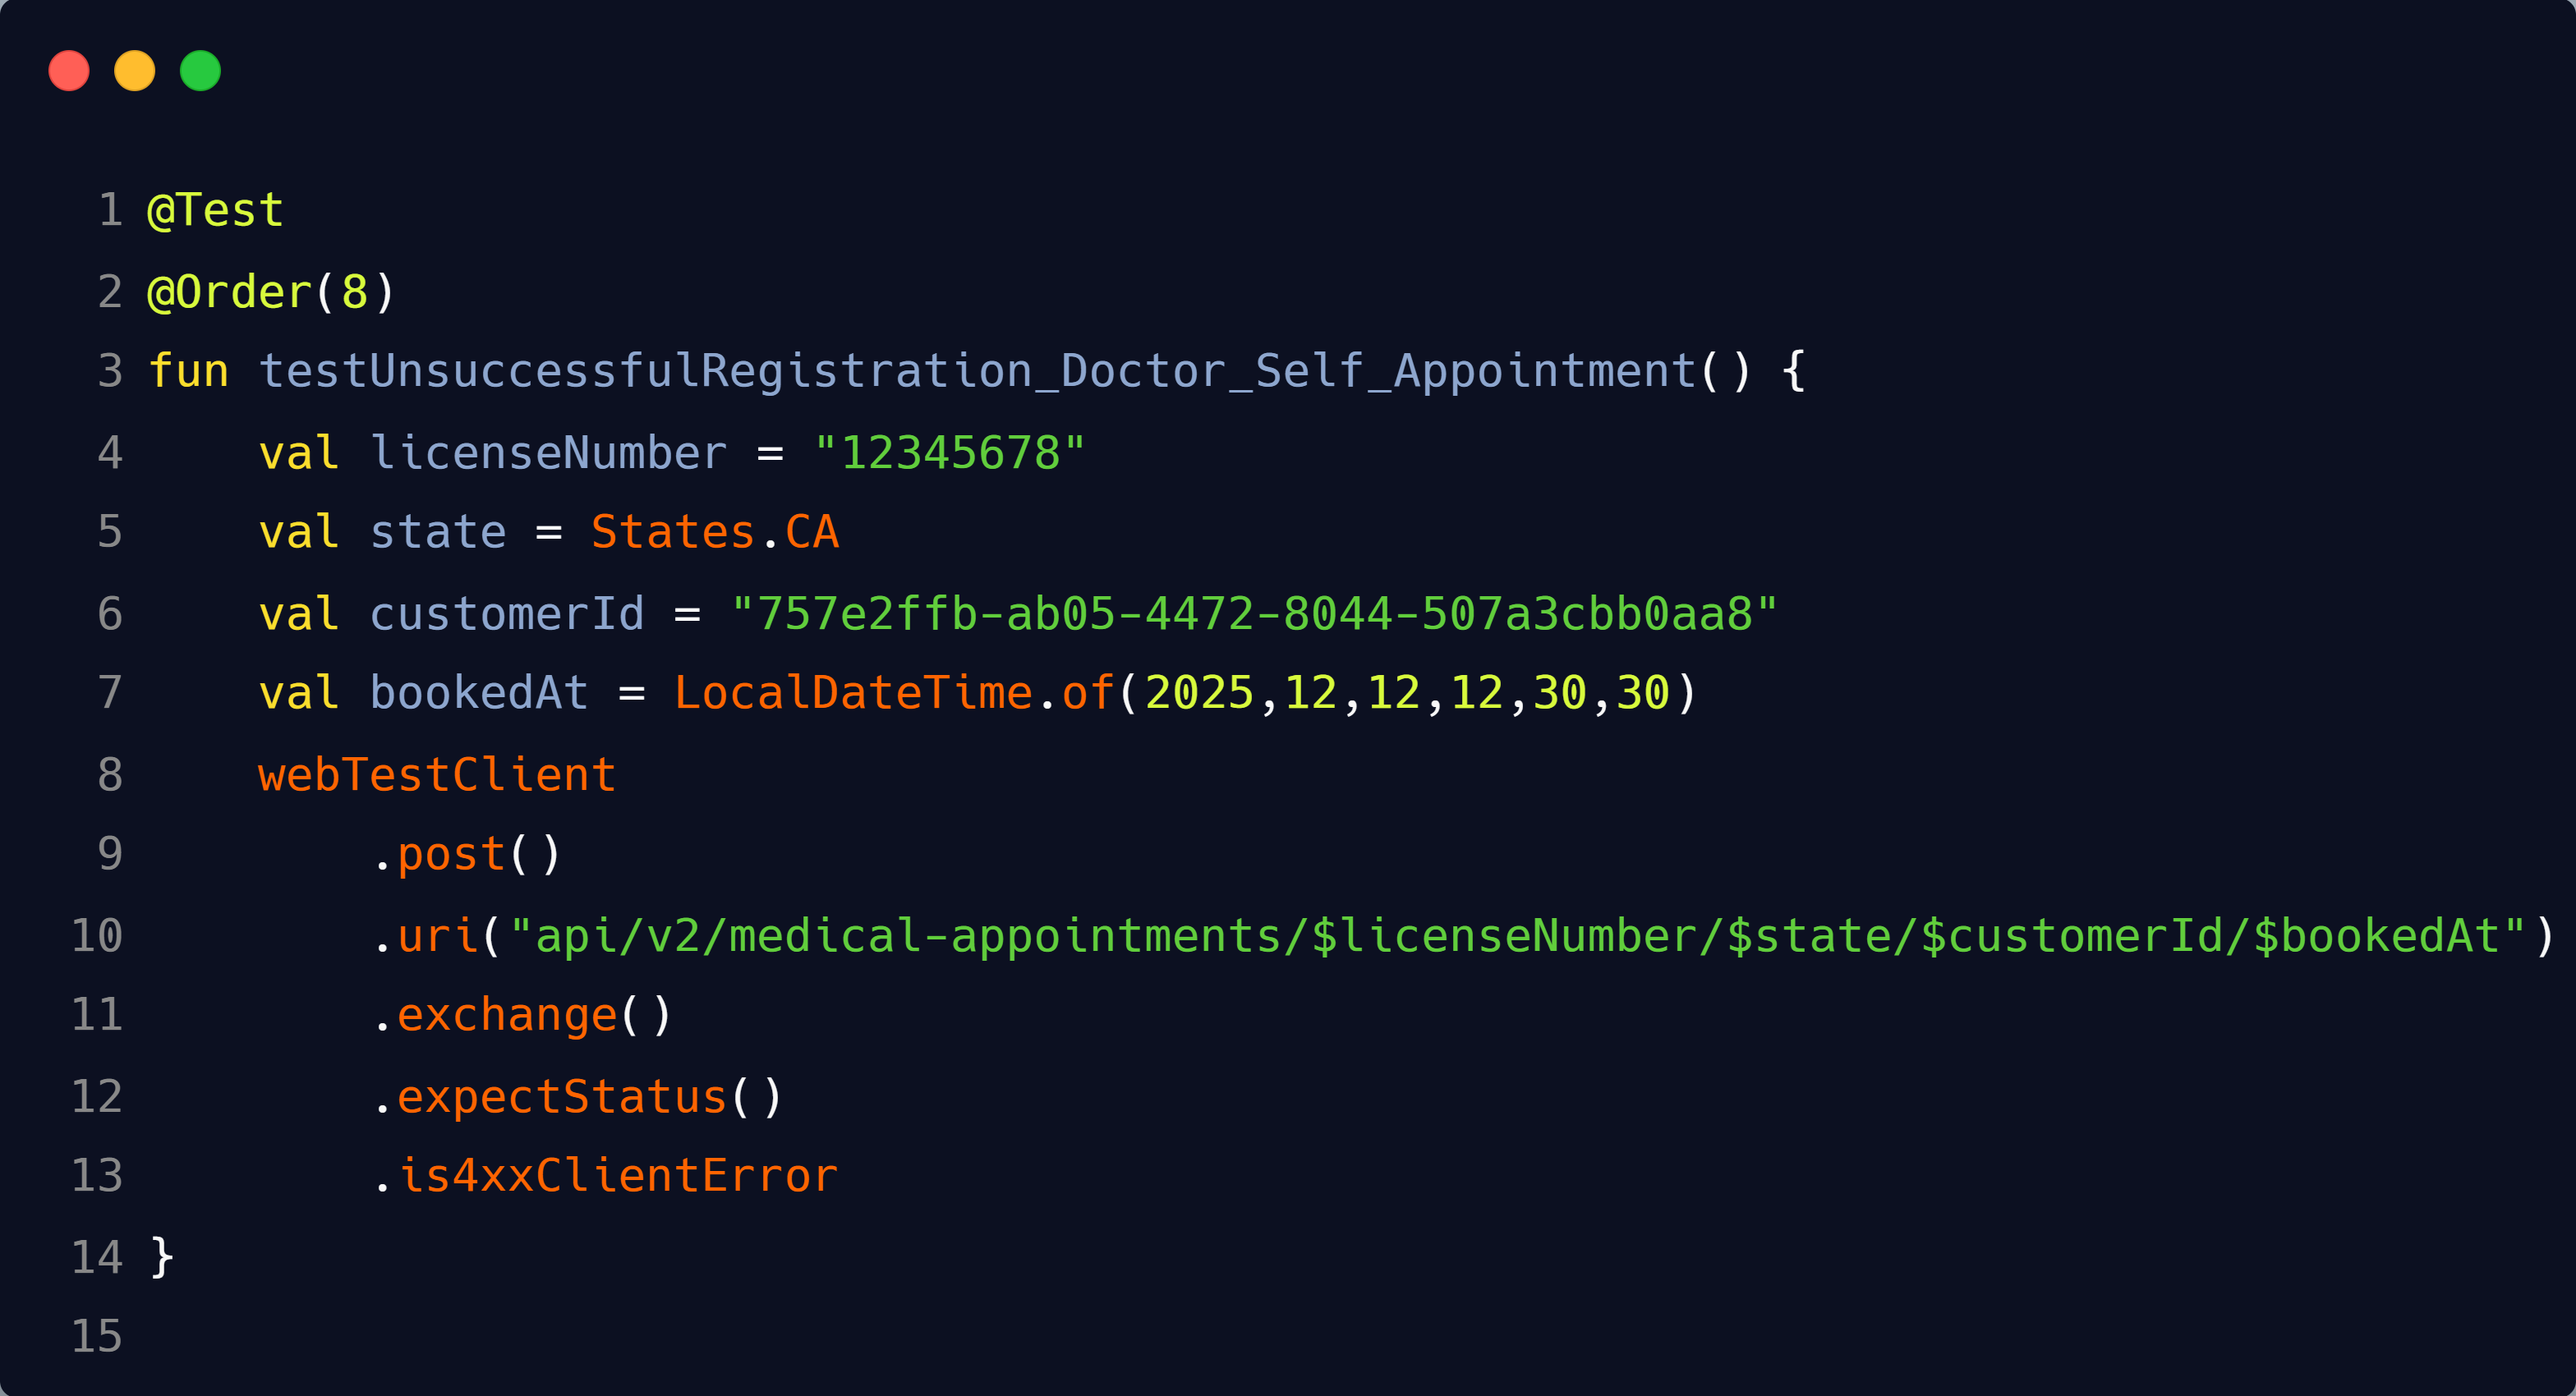
\includegraphics[width=1\linewidth]{figures/medical_appointment_registration_integration_test_unsuccessful_case_doctor_self_booking.png}
	\label{fig:medical_appointment_registration_integration_test_unsuccessful_case_doctor_self_booking}
	\footnotesize Source: Author's creation.
\end{figure}

The method \textit{testUnsuccessfulRegistration\_Doctor\_Self\_Booking} uses an instance of the \textit{WebTestClient}, as argued by the \hyperref[subsection:automated_software_testing]{subsection Automated Software Testing}. When, at the moment that validated input data is extracted from the path variables \textit{customer\_id}, \textit{license\_number}, \textit{state}, and \textit{booked\_at}, and it is discovered that sought \textbf{Customer} is equally the sought \textbf{MedicalSlot}'s doctor, the \hyperref[tab:summary_http_status_codes]{status code 409} is returned.


\subsubsection{Summary of Results}


\begin{figure}[H]
	\centering
	\caption{Medical Appointment Registration Integration Test's Result}
	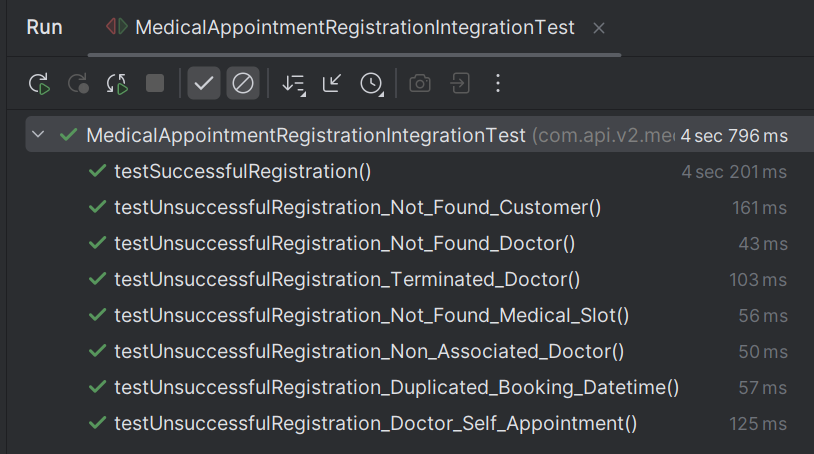
\includegraphics[width=1\linewidth]{figures/medical_appointment_registration_integration_test_results.png}
	\label{fig:medical_appointment_registration_integration_test_results}
	\footnotesize Source: Author's creation.
\end{figure}

As expected, all the results of tests were successful. Methods of integration tests are expected to pass, regardless of successful or unsuccessful representation of the endpoint's response, due to the fact that integration tests are supposed to represent the system's functionality.

\subsection{Medical Appointment Management}

\newpage

\subsection{Medical Appointment's Payment}

The figure \ref{fig:payment_registration_activity_diagram} demonstrates the flow of registering a medical appointment's payment.

\begin{figure}[H]
	\centering
	\caption{Flow of the Payment of Medical Appointment}
	\label{fig:payment_registration_activity_diagram}
	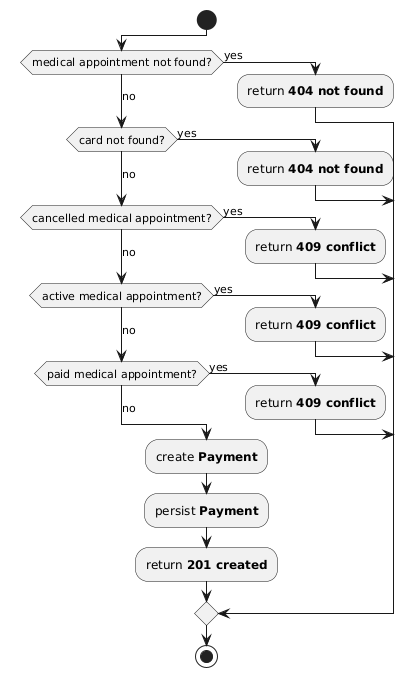
\includegraphics[width=0.7\linewidth]{figures/payment_registration_activity_diagram.png}
	\\ \footnotesize Source: Author's creation.
\end{figure}

When either of the \textbf{MedicalSlot} and \textbf{Card} is null, the \hyperref[tab:summary_http_status_codes]{status code 404} is returned. When the sought \textbf{MedicalAppointment} is canceled, active or paid, the \hyperref[tab:summary_http_status_codes]{status code 409} is returned. As the default behavior, a new instance of \textbf{Payment} is created, persisted. Finally, the \hyperref[tab:summary_http_status_codes]{status code 201} is returned. A more detailed flow is exposed in the sequence diagram(figure \ref{fig:payment_registration_sequence_diagram}).

The client, whose behavior is described in the \hyperref[subsection:http_semantics]{subsection HTTP Semantics}, requests a resource. It uses the \hyperref[appendix:glossary]{URI} \textit{/api/v2/payments/\underline{card\_id}/\underline{medical\_appointments\_id}}. The \hyperref[appendix:glossary]{URI} follows the pattern established  in the table \ref{tab:http-server-schemes}.

The path variables \textit{card\_id}, \textit{medical\_appointments\_id} are passed, respectively, to the \hyperref[appendix:glossary]{URI} \textit{/api/v2/payments/\underline{card\_id}/\underline{medical\_appointments\_id}} as arguments. The service creates a new \textbf{Payment}, then persists it.

As exposed by the figure \ref{fig:payment_registration_activity_diagram}, the default behavior is: firstly, \textbf{Card} must be found. Then, \textbf{MedicalAppointment} is found. To retrieve both \textbf{Card} and \textbf{MedicalAppointment}, the utility classes \textit{CardFinder} and \textit{MedicalAppointmentFinder}, respectively. Finally, a new instance of \textbf{Payment} is created, persisted and wrapped in the \hyperref[tab:summary_http_status_codes]{status code 201}.

Despite the default behavior, when either of the \textbf{MedicalSlot} and \textbf{Card} is null, the \hyperref[tab:summary_http_status_codes]{status code 404} is returned. Additionally, the sought \textbf{MedicalAppointment} is canceled, active or paid, the \hyperref[tab:summary_http_status_codes]{status code 409} is returned.

\begin{figure}[H]
	\centering
	\caption{Medical Appointment's Payment Sequence Diagram}
	\label{fig:payment_registration_sequence_diagram}
	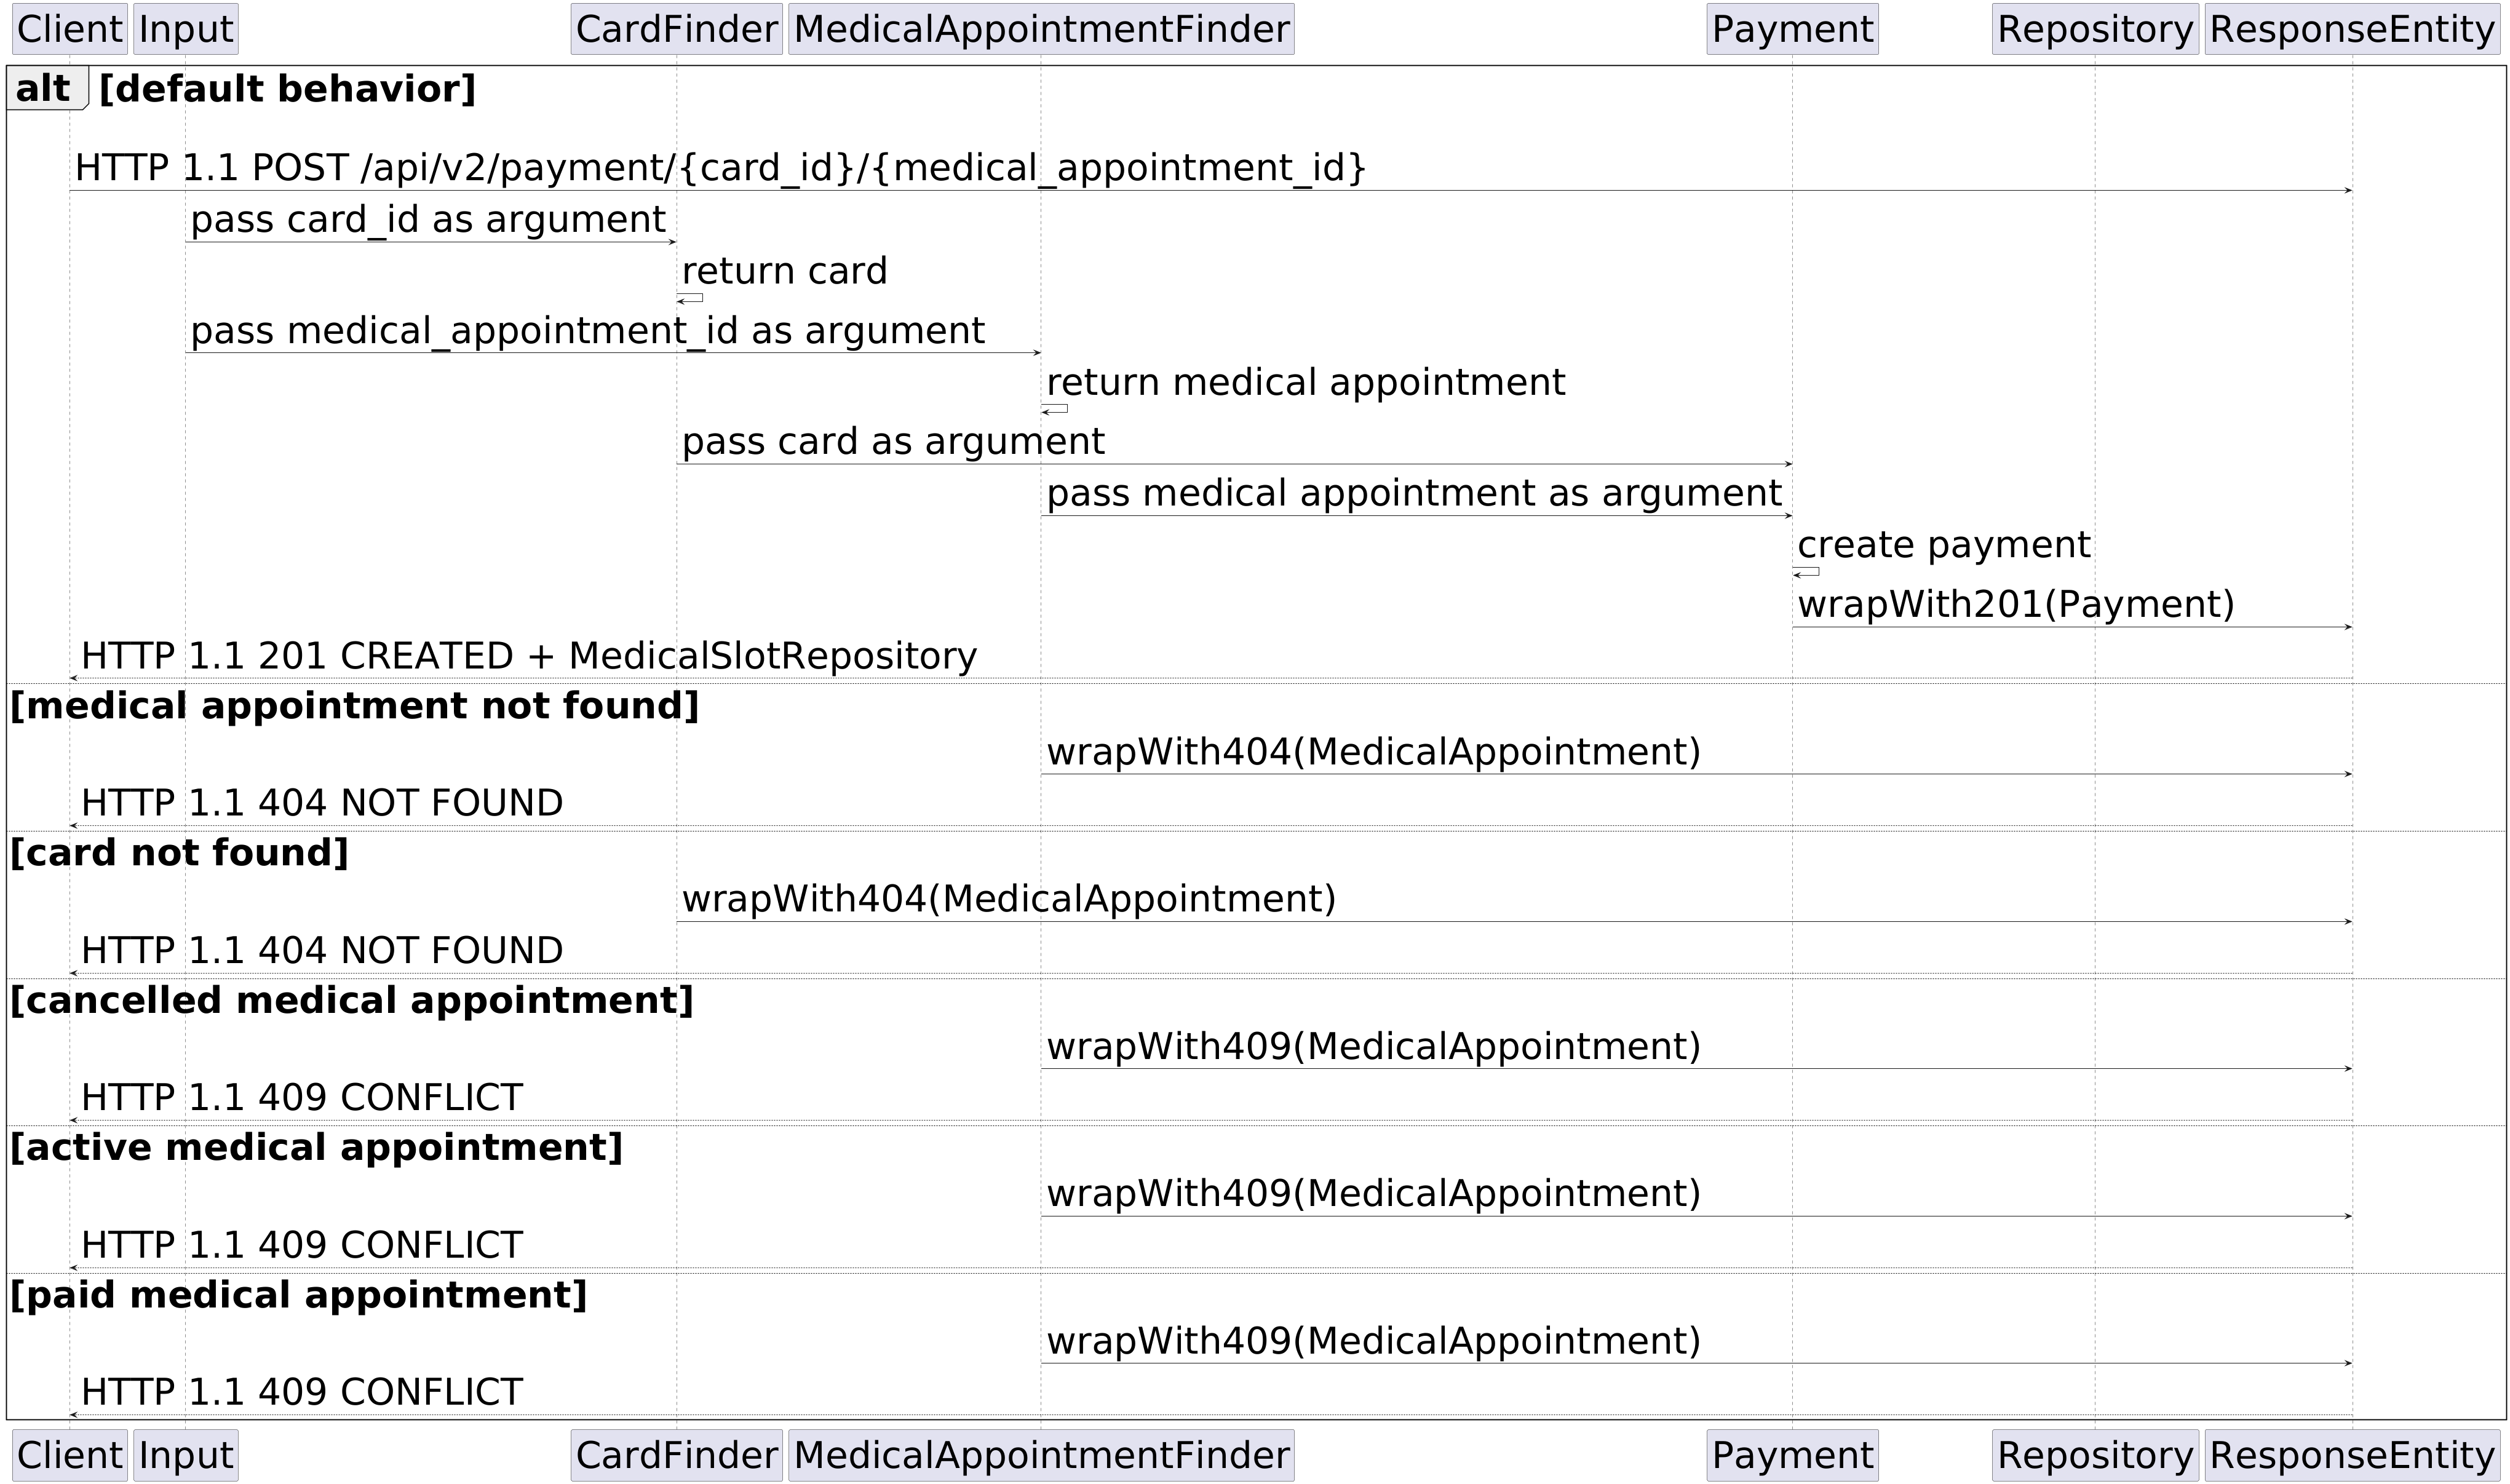
\includegraphics[width=1\linewidth]{figures/payment_registration_sequence_diagram.png}
	\footnotesize Source: Author's creation.	
\end{figure}

\subsubsection{Successful Case}

\begin{figure}[H]
	\centering
	\caption{Medical Apponintment's Payment Integration Test's Successful Case}
	\label{fig:payment_successful_integration_test}
	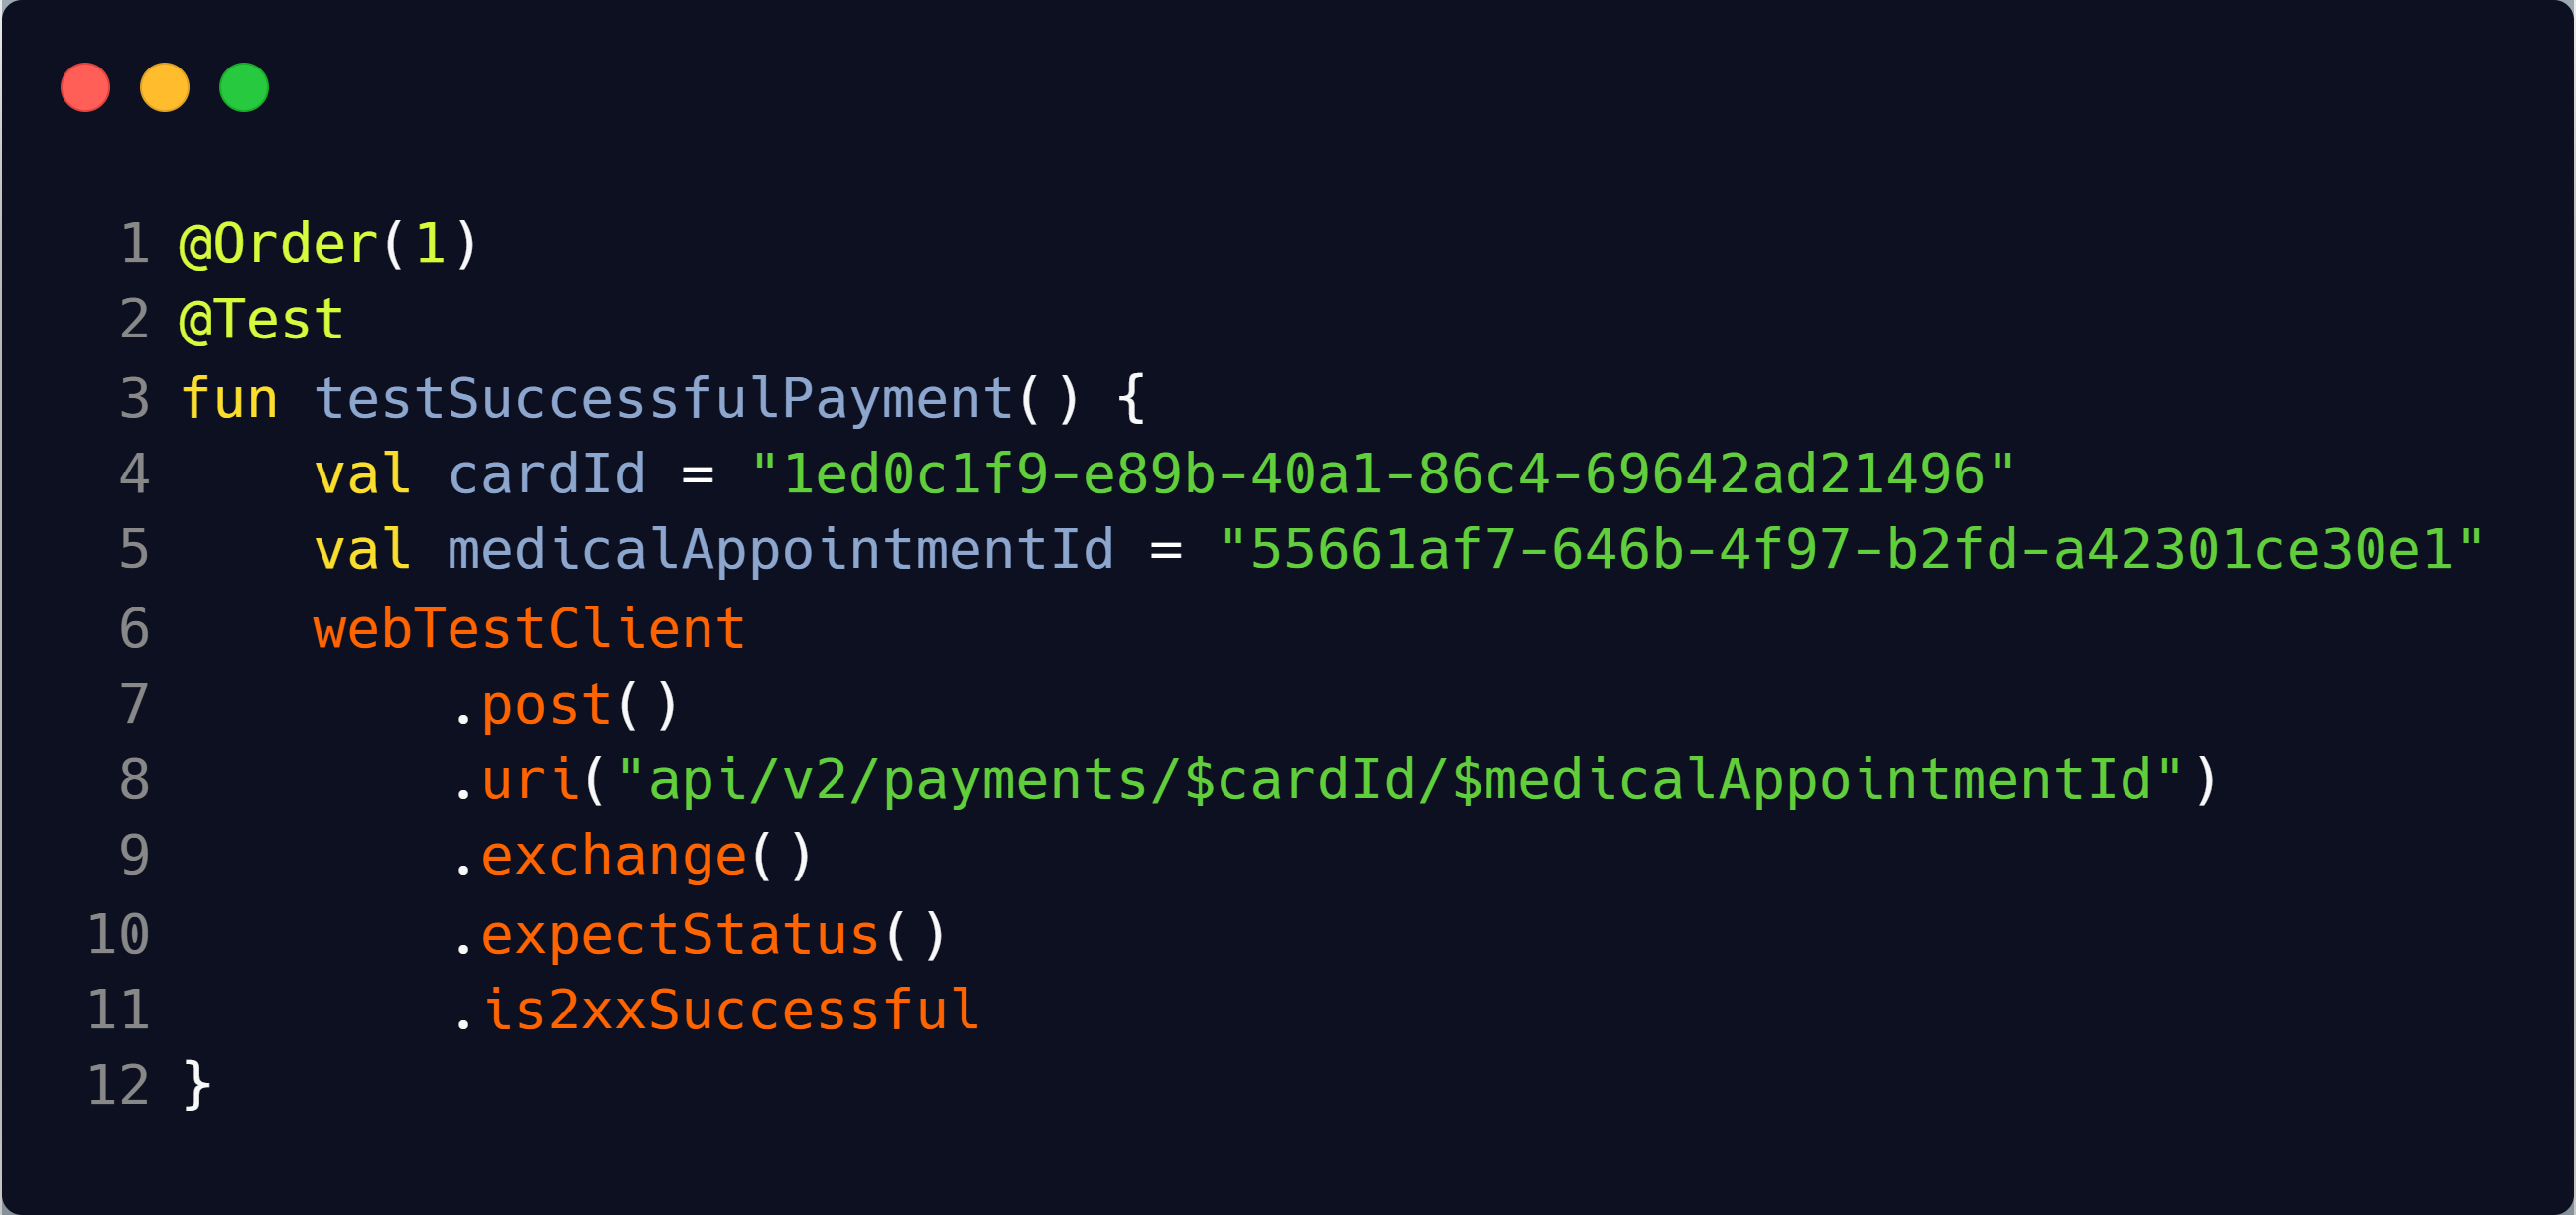
\includegraphics[width=1\linewidth]{figures/payment_successful_integration_test.png}
	\footnotesize Source: Author's creation.
\end{figure}

The method \textit{testSuccessfulRegistration} uses an instance of the \textit{WebTestClient}, as argued by the \hyperref[subsection:automated_software_testing]{subsection Automated Software Testing}. In order to register a \textbf{Payment}, the POST method was used. As clarified by the \hyperref[subsection:http_semantics]{subsection HTTP Semantics}, every HTTP request requires a \hyperref[appendix:glossary]{URI} to route the expected request to the target server aiming to obtain the expected result. Thereby, the \hyperref[appendix:glossary]{URI} \textit{/api/v2/payments/\underline{card\_id}/\underline{medical\_appointment\_id}} is placed as the argument of \textit{uri()}. Finally, the \hyperref[tab:summary_http_status_codes]{status code 201} is returned.

\subsubsection{Unsuccessful Case: Medical Appointment Not Found}

\begin{figure}[H]
	\centering
	\caption{Medical Apponintment's Payment Integration Test's Unsuccessful Case: Medical Appointment Not Found}
	\label{fig:payment_unsuccessful_integration_test_medical_appointment_not_found}
	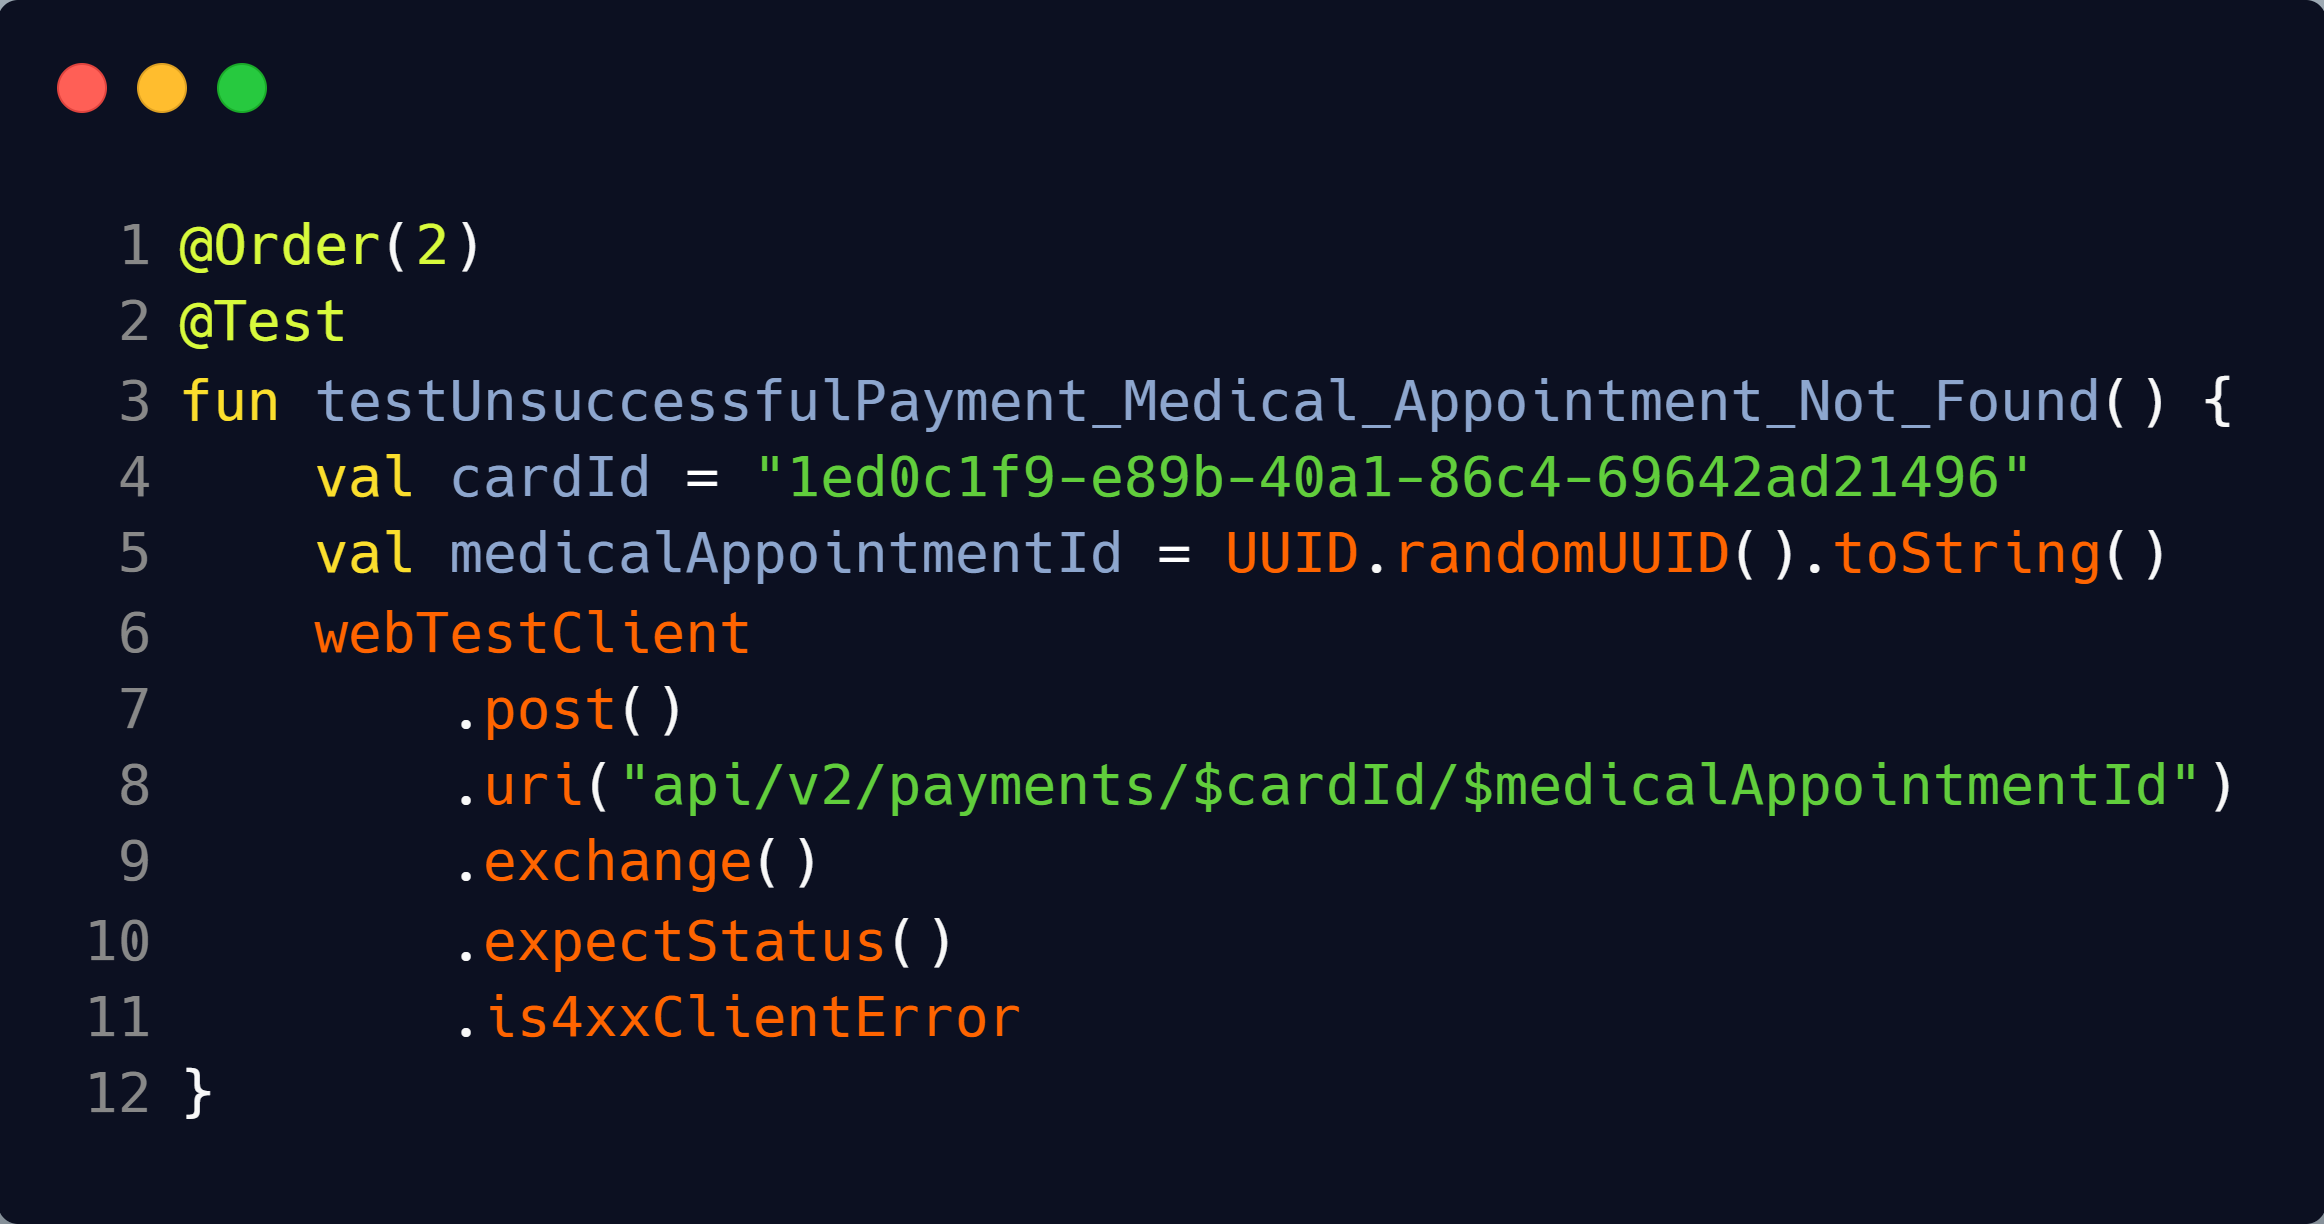
\includegraphics[width=1\linewidth]{figures/payment_unsuccessful_integration_test_medical_appointment_not_found.png}
	\footnotesize Source: Author's creation.
\end{figure}

The method \textit{testUnsuccessfulRegistration\_Medical\_Appointment\_Not\_Found} uses an instance of the \textit{WebTestClient}, as argued by the \hyperref[subsection:automated_software_testing]{subsection Automated Software Testing}. When, at the moment that validated input data is extracted from the path variables \textit{card\_id}  and \textit{medical\_appointment\_id}, and it is discovered that sought \textbf{MedicalAppointment} is null, the \hyperref[tab:summary_http_status_codes]{status code 404} is returned.

\subsubsection{Unsuccessful Case: Card Not Found}

\begin{figure}[H]
	\centering
	\caption{Medical Apponintment's Payment Integration Test's Unsuccessful Case: Card Not Found}
	\label{fig:payment_unsuccessful_integration_test_card_not_founds}
	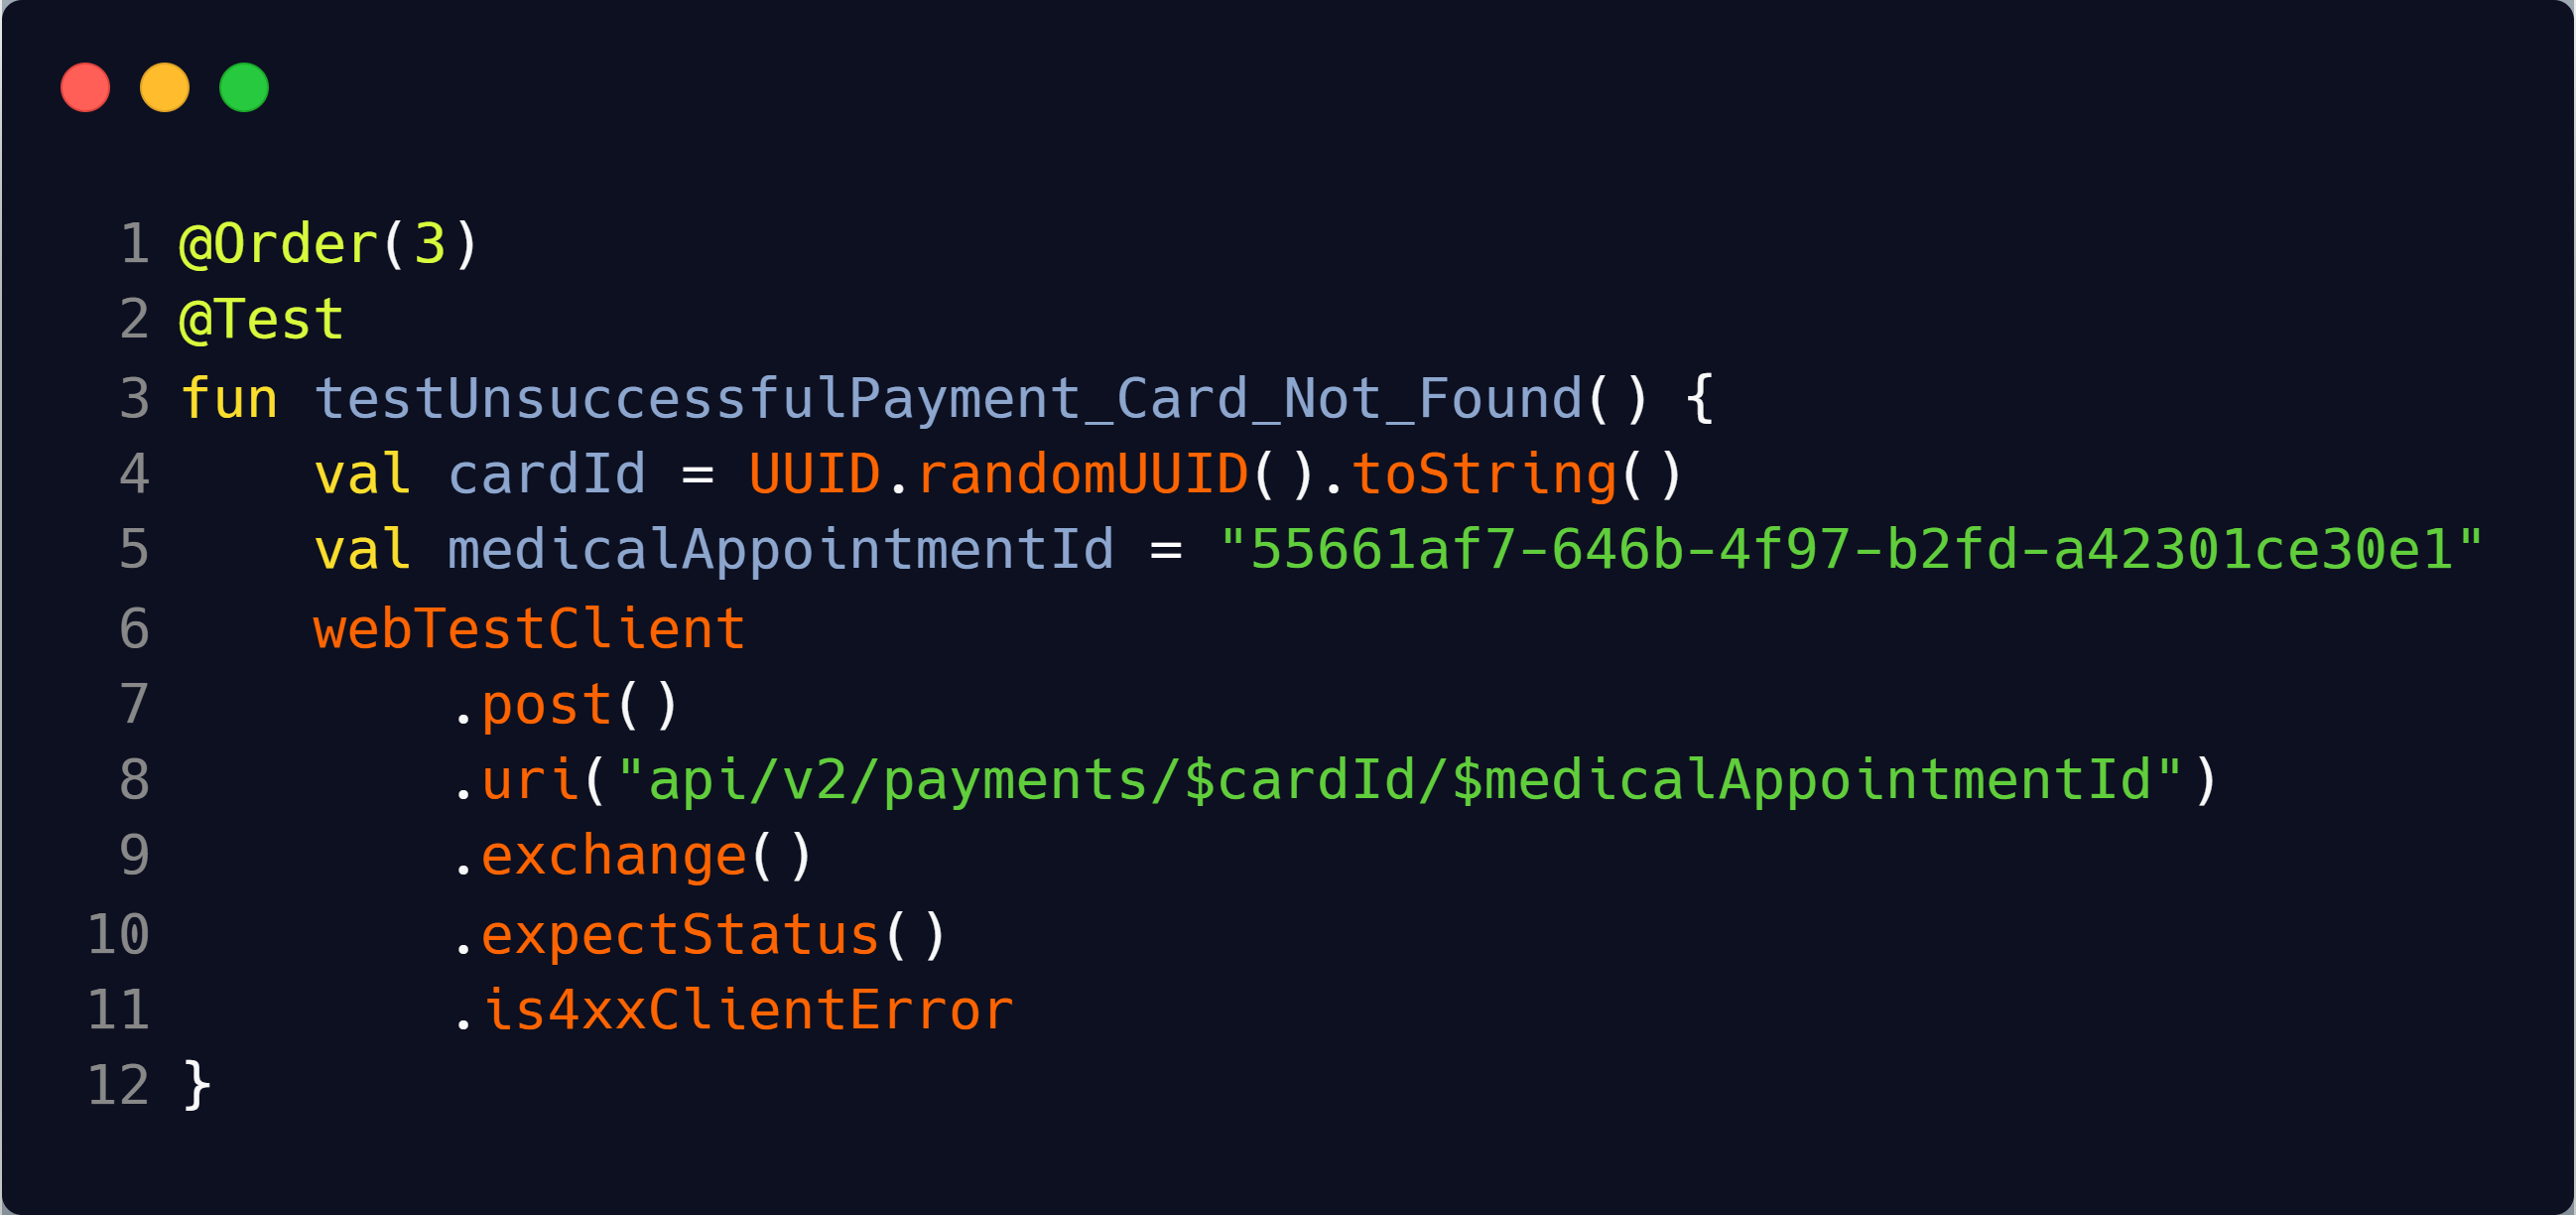
\includegraphics[width=1\linewidth]{figures/payment_unsuccessful_integration_test_card_not_found.png}
	\footnotesize Source: Author's creation.
\end{figure}

The method \textit{testUnsuccessfulRegistration\_Card\_Not\_Found} uses an instance of the \textit{WebTestClient}, as argued by the \hyperref[subsection:automated_software_testing]{subsection Automated Software Testing}. When, at the moment that validated input data is extracted from the path variables \textit{card\_id}  and \textit{medical\_appointment\_id}, and it is discovered that sought \textbf{Card} is null, the \hyperref[tab:summary_http_status_codes]{status code 404} is returned.

\subsubsection{Unsuccessful Case: Currently Canceled Medical Appointment}

\begin{figure}[H]
	\centering
	\caption{Medical Apponintment's Payment Integration Test's Unsuccessful Case: Currently Canceled Medical Appointment}
	\label{fig:payment_unsuccessful_integration_test_canceled_medical_appointment}
	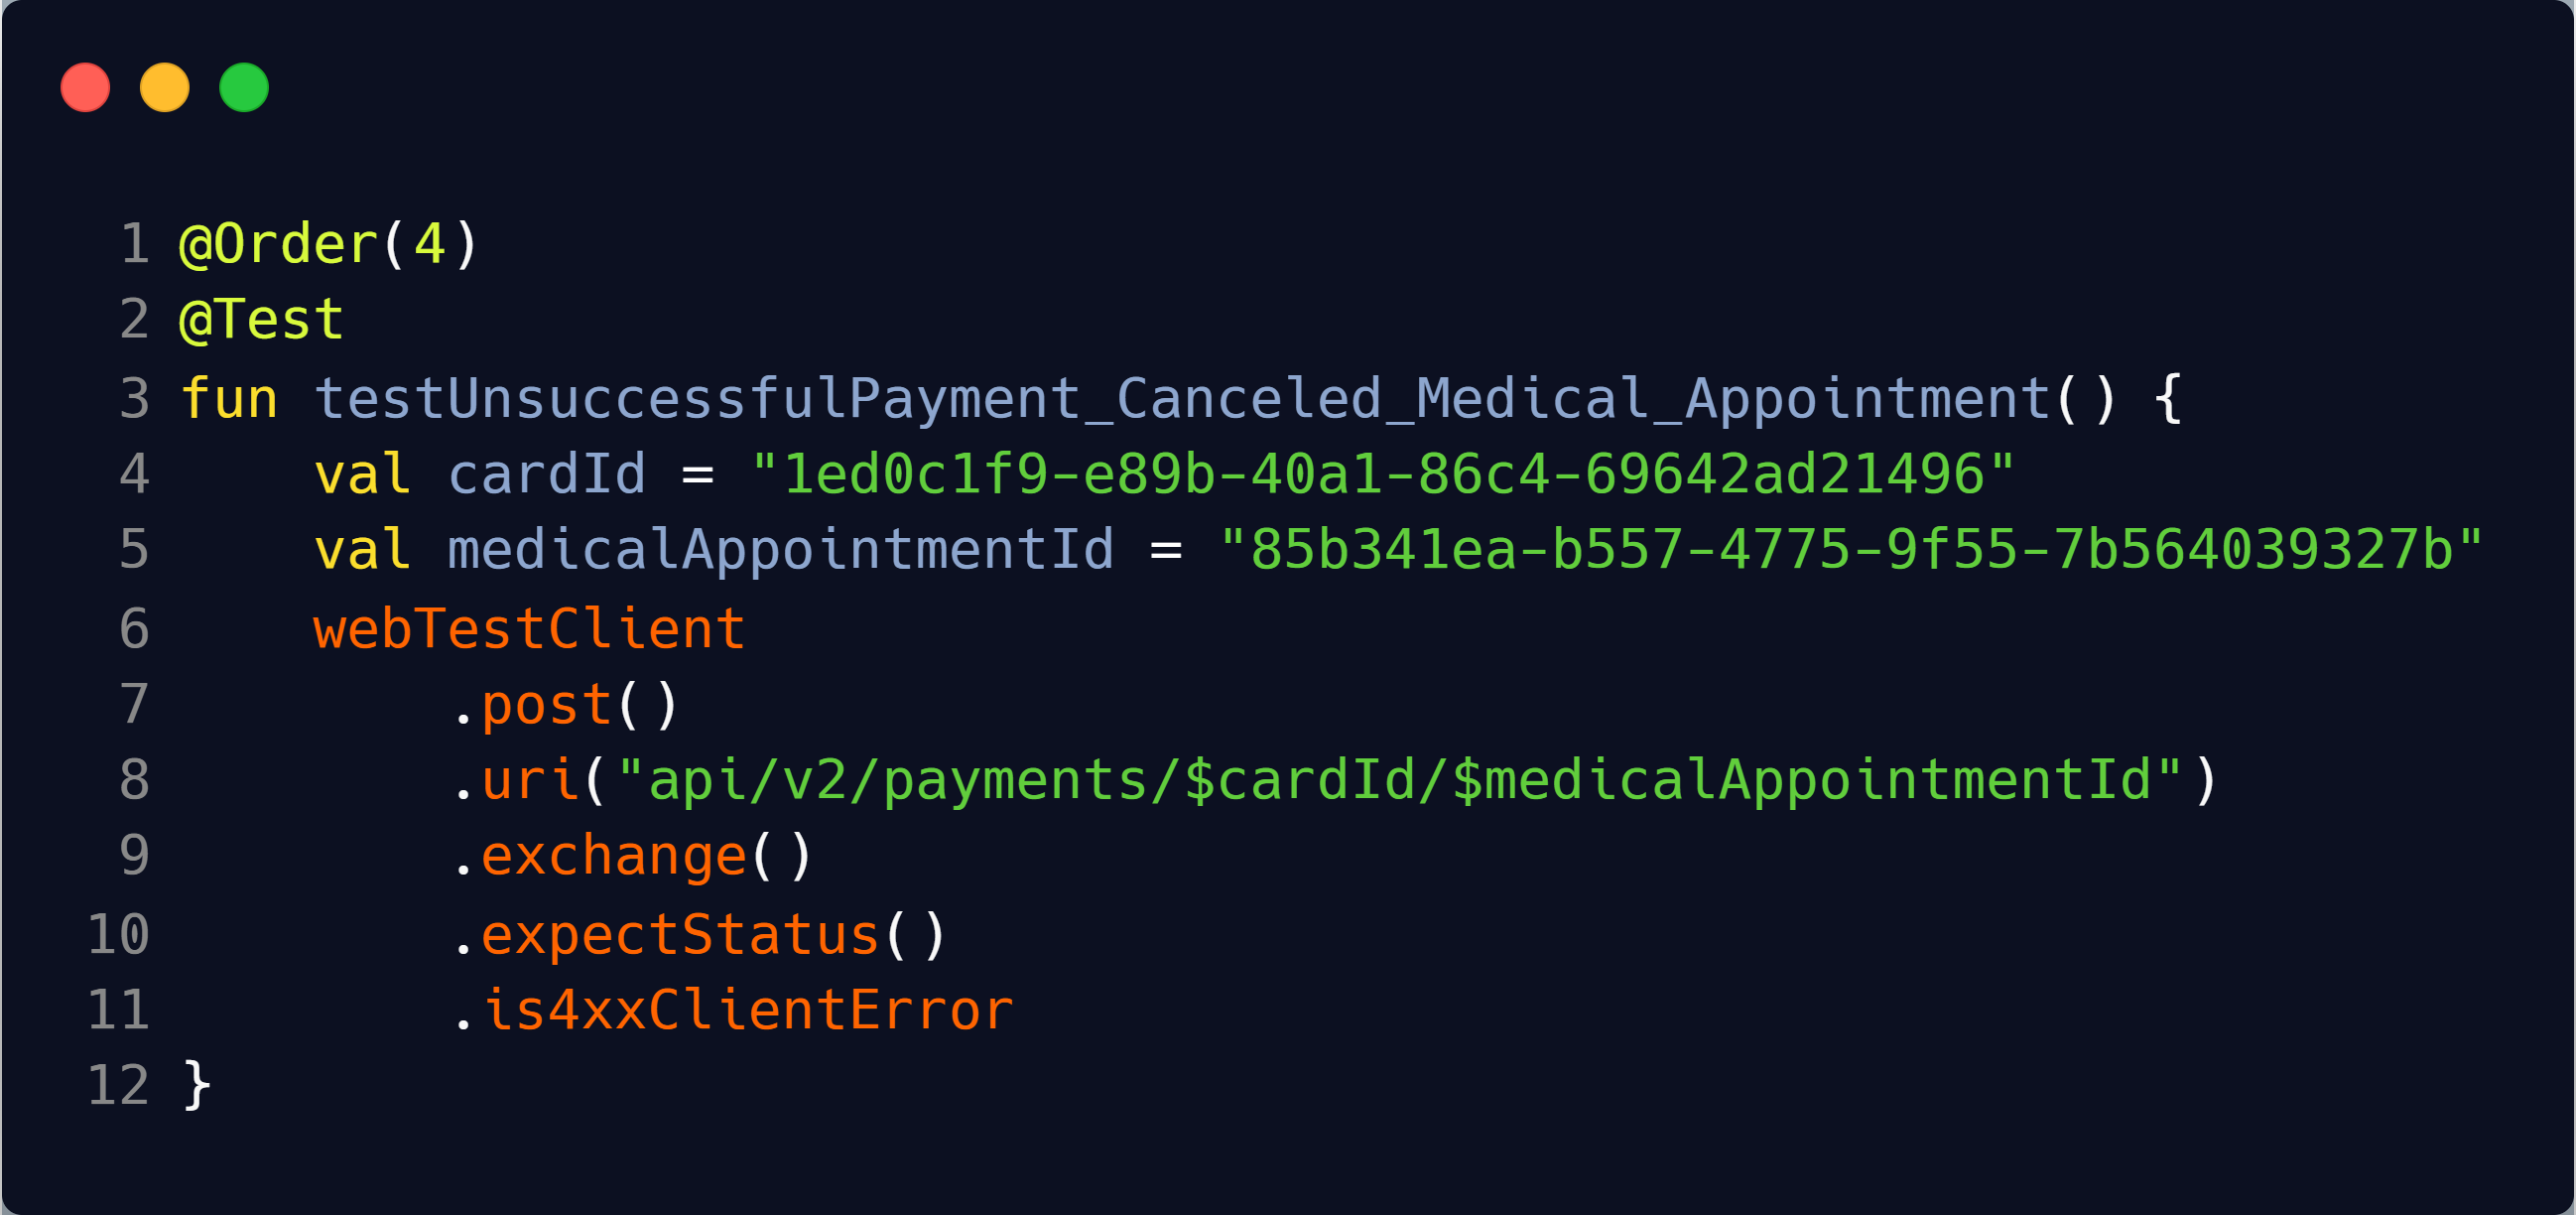
\includegraphics[width=1\linewidth]{figures/payment_unsuccessful_integration_test_canceled_medical_appointment.png}
	\footnotesize Source: Author's creation.
\end{figure}

The method \textit{testUnsuccessfulRegistration\_Canceled\_Medical\_Appointment} uses an instance of the \textit{WebTestClient}, as argued by the \hyperref[subsection:automated_software_testing]{subsection Automated Software Testing}. When, at the moment that validated input data is extracted from the path variables \textit{card\_id}  and \textit{medical\_appointment\_id}, and it is discovered that sought \textbf{MedicalAppointment} is currently canceled, the \hyperref[tab:summary_http_status_codes]{status code 409} is returned.

\subsubsection{Unsuccessful Case: Currently Active Medical Appointment}

\begin{figure}[H]
	\centering
	\caption{Medical Apponintment's Payment Integration Test's Unsuccessful Case: Currently Active Medical Appointment}
	\label{fig:payment_unsuccessful_integration_test_active_medical_appointment}
	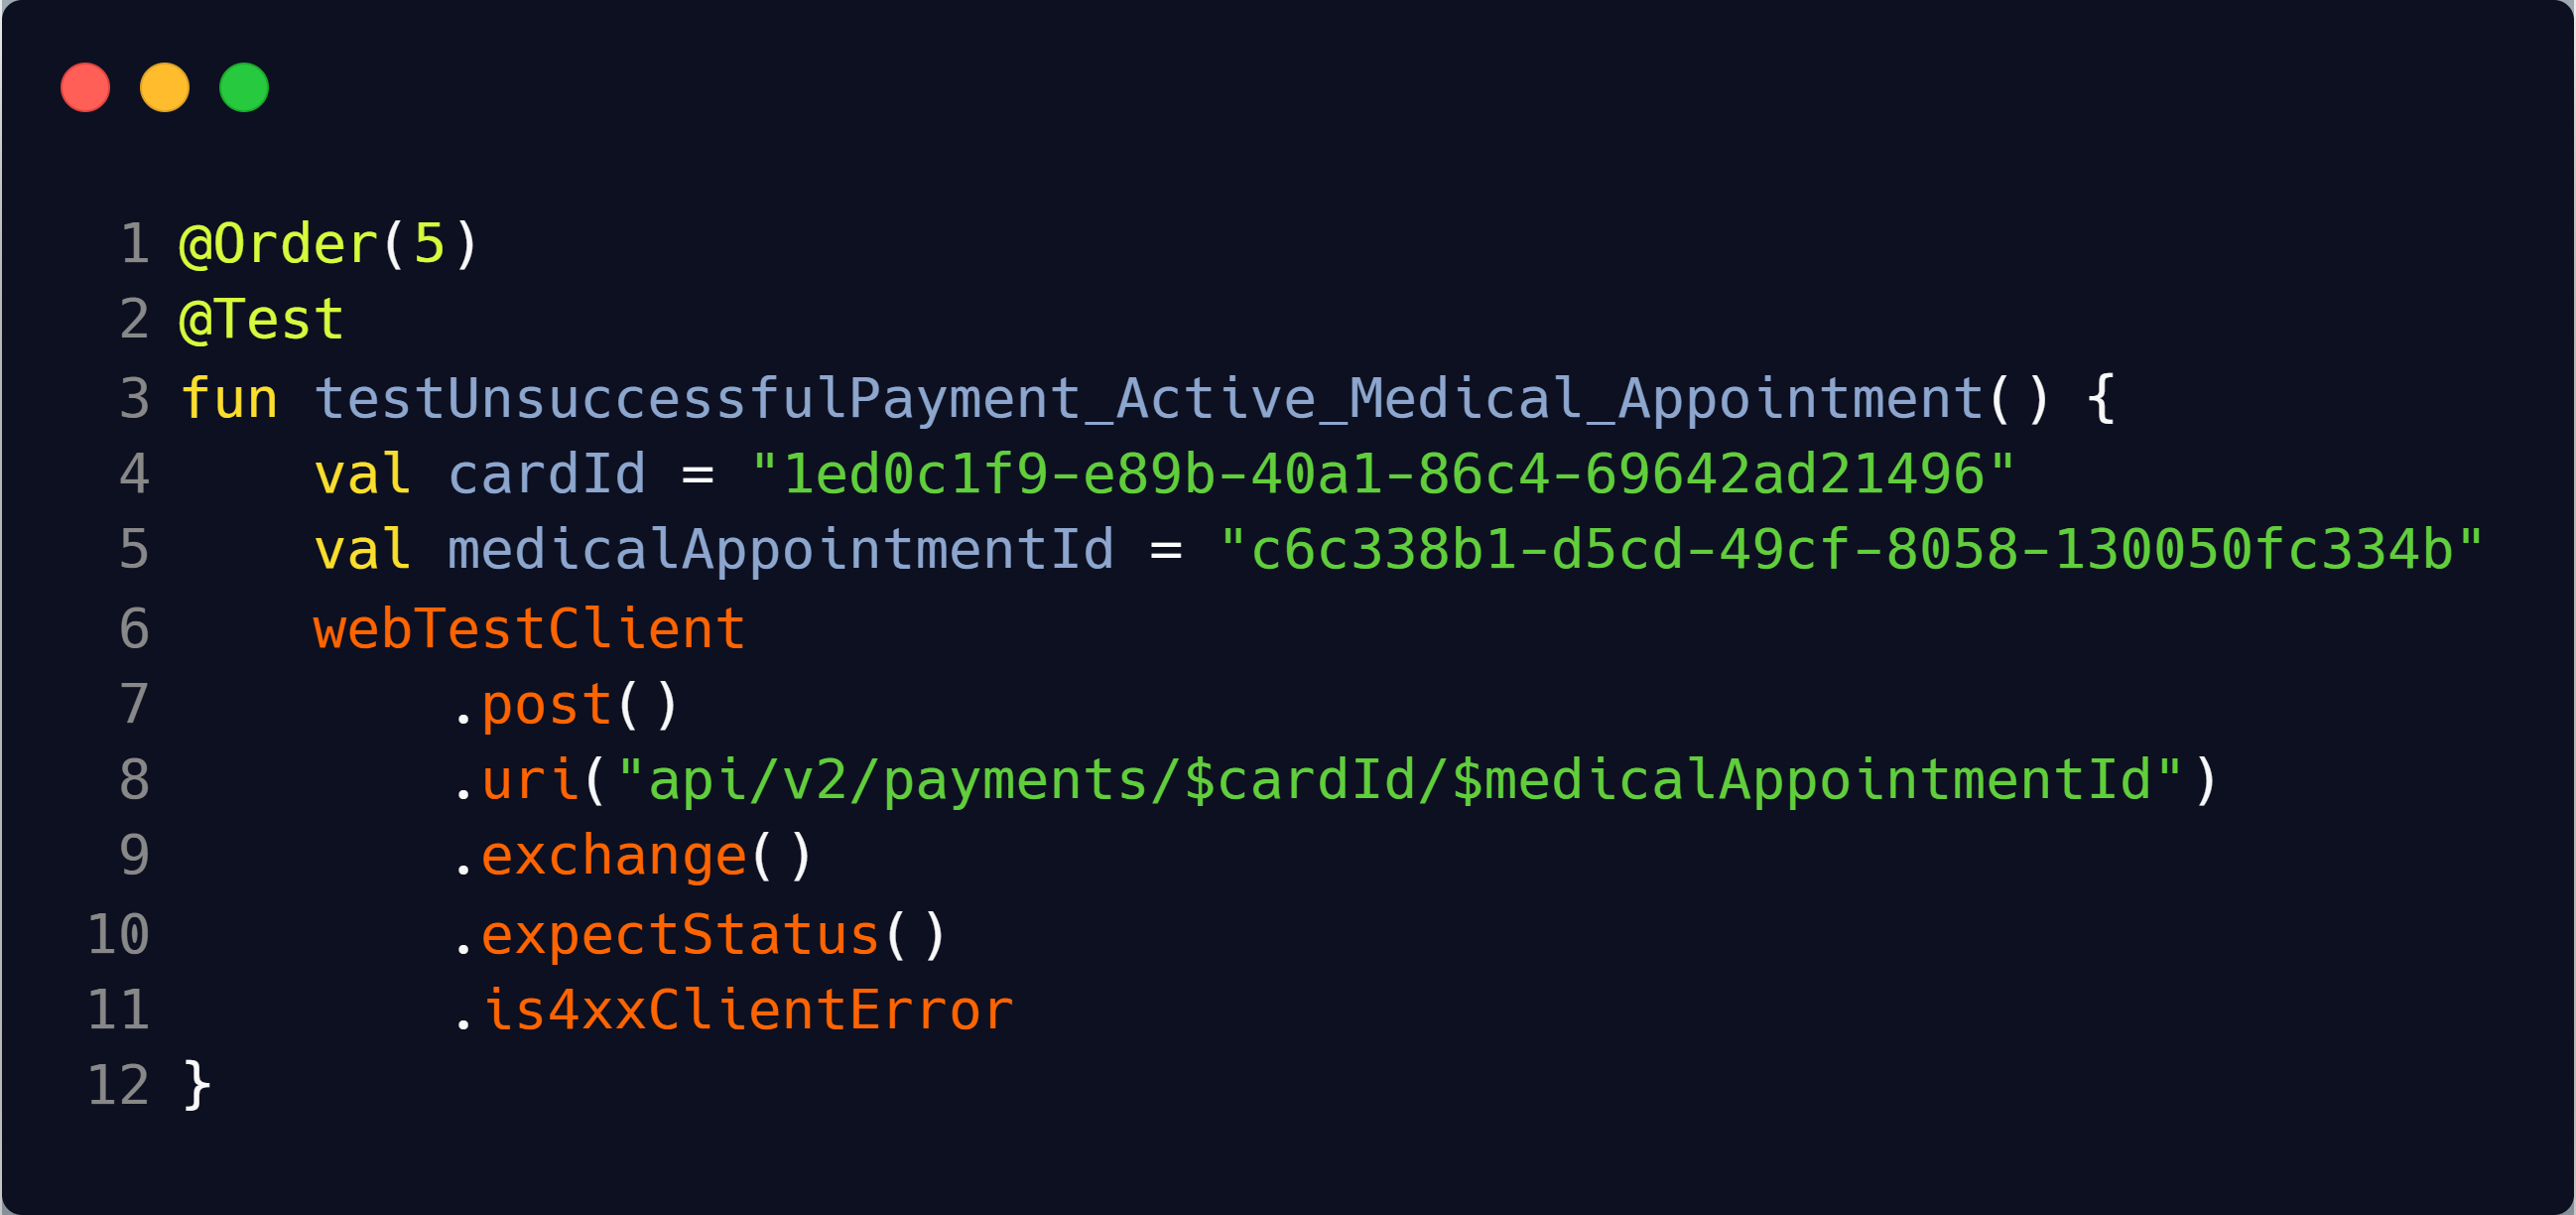
\includegraphics[width=1\linewidth]{figures/payment_unsuccessful_integration_test_active_medical_appointment.png}
	\footnotesize Source: Author's creation.
\end{figure}


The method \textit{testUnsuccessfulRegistration\_Completed\_Medical\_Appointment} uses an instance of the \textit{WebTestClient}, as argued by the \hyperref[subsection:automated_software_testing]{subsection Automated Software Testing}. When, at the moment that validated input data is extracted from the path variables \textit{card\_id}  and \textit{medical\_appointment\_id}, and it is discovered that sought \textbf{MedicalAppointment} is currently active, the \hyperref[tab:summary_http_status_codes]{status code 409} is returned.

\subsubsection{Unsuccessful Case: Currently Paid Medical Appointment}

\begin{figure}[H]
	\centering
	\caption{Medical Apponintment's Payment Integration Test's Unsuccessful Case: Currently Paid Medical Appointment}
	\label{fig:payment_unsuccessful_integration_test_paid_medical_appointment}
	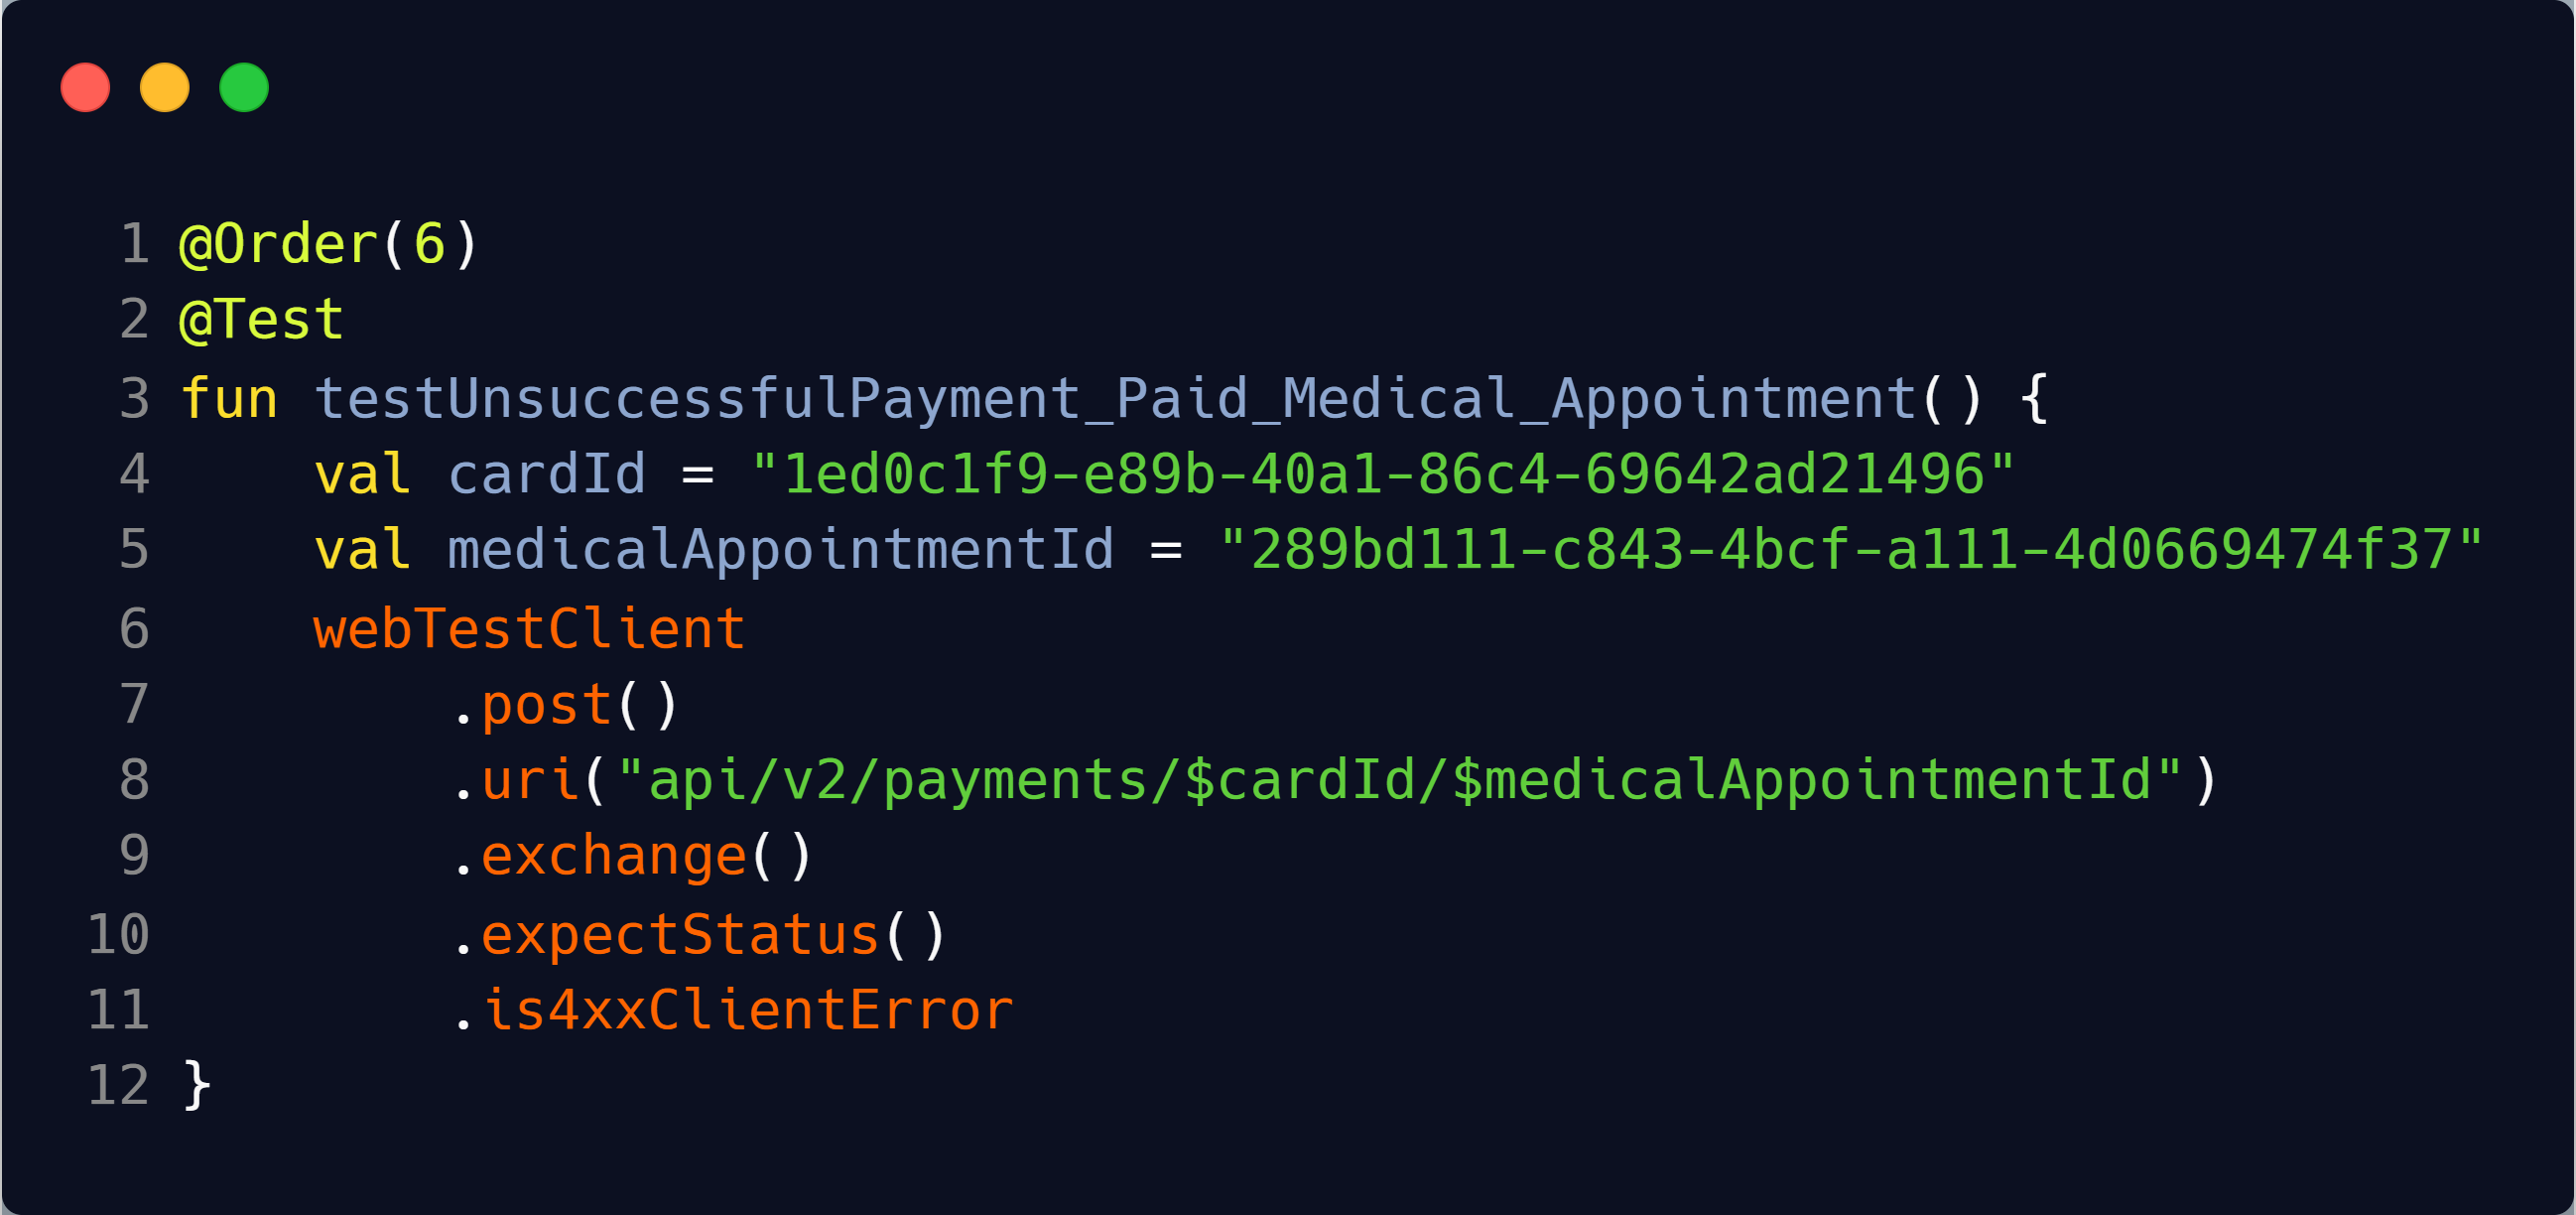
\includegraphics[width=1\linewidth]{figures/payment_unsuccessful_integration_test_paid_medical_appointment.png}
	\footnotesize Source: Author's creation.
\end{figure}

The method \textit{testUnsuccessfulRegistration\_Paid\_Medical\_Appointment} uses an instance of the \textit{WebTestClient}, as argued by the \hyperref[subsection:automated_software_testing]{subsection Automated Software Testing}. When, at the moment that validated input data is extracted from the path variables \textit{card\_id}  and \textit{medical\_appointment\_id}, and it is discovered that sought \textbf{MedicalAppointment} is currently paid, the \hyperref[tab:summary_http_status_codes]{status code 409} is returned.

\subsubsection{Summary of Results}

\begin{figure}[H]
	\centering
	\caption{Medical Apponintment's Payment Integration Test's Results}
	\label{fig:payment_integration_tests_results}
	\includegraphics[width=1\linewidth]{figures/payment_integration_tests_results.png}
	\footnotesize Source: Author's creation.
\end{figure}

As expected, all the results of tests were successful. Methods of integration tests are expected to pass, regardless of successful or unsuccessful representation of the endpoint's response, due to the fact that integration tests are supposed to represent the system's functionality.

\subsection{Medical Slot Management}

\subsection{Medical Appointment Management}